% Options for packages loaded elsewhere
\PassOptionsToPackage{unicode}{hyperref}
\PassOptionsToPackage{hyphens}{url}
%
\documentclass[
]{article}
\usepackage{amsmath,amssymb}
\usepackage{iftex}
\ifPDFTeX
  \usepackage[T1]{fontenc}
  \usepackage[utf8]{inputenc}
  \usepackage{textcomp} % provide euro and other symbols
\else % if luatex or xetex
  \usepackage{unicode-math} % this also loads fontspec
  \defaultfontfeatures{Scale=MatchLowercase}
  \defaultfontfeatures[\rmfamily]{Ligatures=TeX,Scale=1}
\fi
\usepackage{lmodern}
\ifPDFTeX\else
  % xetex/luatex font selection
\fi
% Use upquote if available, for straight quotes in verbatim environments
\IfFileExists{upquote.sty}{\usepackage{upquote}}{}
\IfFileExists{microtype.sty}{% use microtype if available
  \usepackage[]{microtype}
  \UseMicrotypeSet[protrusion]{basicmath} % disable protrusion for tt fonts
}{}
\makeatletter
\@ifundefined{KOMAClassName}{% if non-KOMA class
  \IfFileExists{parskip.sty}{%
    \usepackage{parskip}
  }{% else
    \setlength{\parindent}{0pt}
    \setlength{\parskip}{6pt plus 2pt minus 1pt}}
}{% if KOMA class
  \KOMAoptions{parskip=half}}
\makeatother
\usepackage{xcolor}
\usepackage[margin=1in]{geometry}
\usepackage{color}
\usepackage{fancyvrb}
\newcommand{\VerbBar}{|}
\newcommand{\VERB}{\Verb[commandchars=\\\{\}]}
\DefineVerbatimEnvironment{Highlighting}{Verbatim}{commandchars=\\\{\}}
% Add ',fontsize=\small' for more characters per line
\usepackage{framed}
\definecolor{shadecolor}{RGB}{248,248,248}
\newenvironment{Shaded}{\begin{snugshade}}{\end{snugshade}}
\newcommand{\AlertTok}[1]{\textcolor[rgb]{0.94,0.16,0.16}{#1}}
\newcommand{\AnnotationTok}[1]{\textcolor[rgb]{0.56,0.35,0.01}{\textbf{\textit{#1}}}}
\newcommand{\AttributeTok}[1]{\textcolor[rgb]{0.13,0.29,0.53}{#1}}
\newcommand{\BaseNTok}[1]{\textcolor[rgb]{0.00,0.00,0.81}{#1}}
\newcommand{\BuiltInTok}[1]{#1}
\newcommand{\CharTok}[1]{\textcolor[rgb]{0.31,0.60,0.02}{#1}}
\newcommand{\CommentTok}[1]{\textcolor[rgb]{0.56,0.35,0.01}{\textit{#1}}}
\newcommand{\CommentVarTok}[1]{\textcolor[rgb]{0.56,0.35,0.01}{\textbf{\textit{#1}}}}
\newcommand{\ConstantTok}[1]{\textcolor[rgb]{0.56,0.35,0.01}{#1}}
\newcommand{\ControlFlowTok}[1]{\textcolor[rgb]{0.13,0.29,0.53}{\textbf{#1}}}
\newcommand{\DataTypeTok}[1]{\textcolor[rgb]{0.13,0.29,0.53}{#1}}
\newcommand{\DecValTok}[1]{\textcolor[rgb]{0.00,0.00,0.81}{#1}}
\newcommand{\DocumentationTok}[1]{\textcolor[rgb]{0.56,0.35,0.01}{\textbf{\textit{#1}}}}
\newcommand{\ErrorTok}[1]{\textcolor[rgb]{0.64,0.00,0.00}{\textbf{#1}}}
\newcommand{\ExtensionTok}[1]{#1}
\newcommand{\FloatTok}[1]{\textcolor[rgb]{0.00,0.00,0.81}{#1}}
\newcommand{\FunctionTok}[1]{\textcolor[rgb]{0.13,0.29,0.53}{\textbf{#1}}}
\newcommand{\ImportTok}[1]{#1}
\newcommand{\InformationTok}[1]{\textcolor[rgb]{0.56,0.35,0.01}{\textbf{\textit{#1}}}}
\newcommand{\KeywordTok}[1]{\textcolor[rgb]{0.13,0.29,0.53}{\textbf{#1}}}
\newcommand{\NormalTok}[1]{#1}
\newcommand{\OperatorTok}[1]{\textcolor[rgb]{0.81,0.36,0.00}{\textbf{#1}}}
\newcommand{\OtherTok}[1]{\textcolor[rgb]{0.56,0.35,0.01}{#1}}
\newcommand{\PreprocessorTok}[1]{\textcolor[rgb]{0.56,0.35,0.01}{\textit{#1}}}
\newcommand{\RegionMarkerTok}[1]{#1}
\newcommand{\SpecialCharTok}[1]{\textcolor[rgb]{0.81,0.36,0.00}{\textbf{#1}}}
\newcommand{\SpecialStringTok}[1]{\textcolor[rgb]{0.31,0.60,0.02}{#1}}
\newcommand{\StringTok}[1]{\textcolor[rgb]{0.31,0.60,0.02}{#1}}
\newcommand{\VariableTok}[1]{\textcolor[rgb]{0.00,0.00,0.00}{#1}}
\newcommand{\VerbatimStringTok}[1]{\textcolor[rgb]{0.31,0.60,0.02}{#1}}
\newcommand{\WarningTok}[1]{\textcolor[rgb]{0.56,0.35,0.01}{\textbf{\textit{#1}}}}
\usepackage{graphicx}
\makeatletter
\newsavebox\pandoc@box
\newcommand*\pandocbounded[1]{% scales image to fit in text height/width
  \sbox\pandoc@box{#1}%
  \Gscale@div\@tempa{\textheight}{\dimexpr\ht\pandoc@box+\dp\pandoc@box\relax}%
  \Gscale@div\@tempb{\linewidth}{\wd\pandoc@box}%
  \ifdim\@tempb\p@<\@tempa\p@\let\@tempa\@tempb\fi% select the smaller of both
  \ifdim\@tempa\p@<\p@\scalebox{\@tempa}{\usebox\pandoc@box}%
  \else\usebox{\pandoc@box}%
  \fi%
}
% Set default figure placement to htbp
\def\fps@figure{htbp}
\makeatother
\setlength{\emergencystretch}{3em} % prevent overfull lines
\providecommand{\tightlist}{%
  \setlength{\itemsep}{0pt}\setlength{\parskip}{0pt}}
\setcounter{secnumdepth}{-\maxdimen} % remove section numbering
\usepackage{bookmark}
\IfFileExists{xurl.sty}{\usepackage{xurl}}{} % add URL line breaks if available
\urlstyle{same}
\hypersetup{
  pdftitle={Untitled},
  hidelinks,
  pdfcreator={LaTeX via pandoc}}

\title{Untitled}
\author{}
\date{\vspace{-2.5em}2026-05-08}

\begin{document}
\maketitle

\subsection*{\texorpdfstring{Accedé al curso completo
\href{curso_completo/curso_completo.qmd}{aquí}}{Accedé al curso completo aquí}}\label{acceduxe9-al-curso-completo-aquuxed}
\addcontentsline{toc}{subsection}{Accedé al curso completo
\href{curso_completo/curso_completo.qmd}{aquí}}

\subsection*{\texorpdfstring{Descarga el material del curso
\href{https://github.com/andresblanco-unc/curso_graficos_ggplot_2026/raw/refs/heads/main/archivos_curso_ggplot_2026.rar}{aquí}}{Descarga el material del curso aquí}}\label{descarga-el-material-del-curso-aquuxed}
\addcontentsline{toc}{subsection}{Descarga el material del curso
\href{https://github.com/andresblanco-unc/curso_graficos_ggplot_2026/raw/refs/heads/main/archivos_curso_ggplot_2026.rar}{aquí}}

\subsection*{Bibliografía
recomendada}\label{bibliografuxeda-recomendada}
\addcontentsline{toc}{subsection}{Bibliografía recomendada}

\begin{itemize}
\tightlist
\item
  Carmona, D.; Benitez-Vieyra, S. Guía de campo de R.
  \href{https://wiki.imbiv.unc.edu.ar/index.php?title=Guía_de_campo_de_R}{Link}
\item
  Chang, W. (2018). R graphics cookbook: practical recipes for
  visualizing data. O'Reilly Media.
  \href{http://www.cookbook-r.com/}{Link}
\item
  Ggplot2 Reference.
  \href{https://ggplot2.tidyverse.org/reference/}{Link}
\item
  Morales, J. Modelos estadísticos, una versión aplicada en R.
  \href{https://bookdown.org/j_morales/librostat/}{Link}
\item
  R-Charts. Gráficos con el paquete ggplot2.
  \href{https://r-charts.com/es/ggplot2/}{Link}
\item
  Tidyverse. \href{https://www.tidyverse.org/}{Link}
\item
  Wickham, H.; Çetinkaya-Rundel, M.; Grolemund, G. (2023). R for data
  science. O'Reilly Media. \href{https://r4ds.hadley.nz/}{Link}
\end{itemize}

\begin{center}\rule{0.5\linewidth}{0.5pt}\end{center}

\subsubsection*{Otros cursos orientados al uso de
R}\label{otros-cursos-orientados-al-uso-de-r}
\addcontentsline{toc}{subsubsection}{Otros cursos orientados al uso de
R}

En el Doctorado de Ciencias Biológicas (FCEFyN, Universidad Nacional de
Córdoba), se dictan con regularidad cursos introductorios y avanzados de
modelos estadísticos en R:

\begin{itemize}
\tightlist
\item
  \textbf{Introducción al lenguaje R. Modelos lineales y fundamentos de
  programación}. \href{https://curso-statscba.github.io/curso-R/}{Ver
  curso}
\item
  \textbf{Modelos Estadísticos Avanzados}.
  \href{https://curso-statscba.github.io/modelos_avanzados/}{Ver curso}
\item
  \textbf{Fundamentos básicos del lenguaje R}.
  \href{https://pastornicolas.github.io/fundamentos_R/}{Ver curso}
\end{itemize}

\begin{center}\rule{0.5\linewidth}{0.5pt}\end{center}

\subsection*{Licencia}\label{licencia}
\addcontentsline{toc}{subsection}{Licencia}

© 2026 Andrés Blanco. Bajo licencia
\href{http://creativecommons.org/licenses/by-nc-sa/4.0/}{Creative
Commons Attribution-NonCommercial-ShareAlike 4.0 International License}.

\href{http://creativecommons.org/licenses/by-nc-sa/4.0/}{\pandocbounded{\includegraphics[keepaspectratio]{https://licensebuttons.net/l/by-nc-sa/4.0/88x31.png}}}

\section*{Objetivos}\label{objetivos}
\addcontentsline{toc}{section}{Objetivos}

El objetivo principal del curso es que los asistentes obtengan
herramientas para la generación y manejo de gráficos utilizando lenguaje
R y el software RStudio, con especial énfasis en la escritura de capas
que requiere el paquete ggplot2.

\section*{Contenidos}\label{contenidos}
\addcontentsline{toc}{section}{Contenidos}

\begin{enumerate}
\def\labelenumi{\arabic{enumi}.}
\tightlist
\item
  Unidad 1. Introducción a R y RStudio. Presentación de los programas.
  Estructura del script de trabajo. Carga de datos y librerías.
  Caracterización analítica y gráfica de las variables. Tipos de
  objetos. Paquete dplyr para manejo y conversión de las bases de
  datos.\\
\item
  Unidad 2. Análisis y representación de datos numéricos. Correlación
  lineal en R. Gráficos de correlaciones. Regresión lineal. Gráficos de
  supuestos. Gráficos de puntos: función plot y lineplot.CI. Manejo de
  parámetros gráficos. Ggplot2: introducción al paquete, gráficos de
  puntos y líneas. Gráfica del modelo lineal. Cálculos de media y desvío
  estándar para gráficos.
\item
  Unidad 3. Análisis y representación de datos categóricos. ANOVA a 1
  factor y bifactorial. Pruebas de supuestos y test a posteriori.
  Gráficos de barras: función bargraph.CI y geom\_col.~Gráficos de
  cajas: función boxplot y geom\_boxplot. Manejo de escalas e
  incorporación de resultados estadísticos.
\item
  Unidad 4. Estructura y estética de gráficos con ggplot2. Estructura
  por capas. Faceting y división por factores. Definición del theme.
  Manipulación de la base de datos a graficar. Escalas de colores, uso
  de paletas. Clasificación por color, tipo de línea y forma.
  Combinación de gráficos: funciones layout, grid.arrange y paquete
  patchwork.
\item
  Unidad 5. Otros tipos y parámetros gráficos. Gráficos de áreas.
  Combinación de distintos geoms. Eje secundario. Pivoteo de bases de
  datos. Gráficos de biplot para análisis de componentes principales.
  Exportación de gráficos: devices y ggsave. Manipulación externa de
  gráficos.
\end{enumerate}

\section{Introducción a R y
RStudio}\label{introducciuxf3n-a-r-y-rstudio}

\subsection{El lenguaje R}\label{el-lenguaje-r}

R es un lenguaje de escritura propio. Como todo lenguaje, tiene la gran
virtud de que permite la comunicación a través de él, se puede
intercambiar, podemos ``hablarlo'' en todas partes del mundo, compartir
\emph{scripts} con colegas y mostrarles cómo analizamos los datos. Sin
embargo, su principal virtud es también su kryptonita ya que, como todo
lenguaje, tiene muchos modismos. Cada persona desarrolla su propia forma
de escritura, arma los \emph{scripts} como le parece conveniente,
entendible, práctico. Uno mismo a lo largo del tiempo va perfeccionando
sus propios escritos, corrigiendo lo antes hecho, reescribiendo con un
estilo más refinado o más avanzado.

Mi reflexión a este respecto es que la experiencia con el software es
dinámica, aquí no se pretende mostrar una receta cerrada que no se puede
modificar (ni mucho menos), sino simplemente acercar el programa a
aquellos que aún no lo conocen y permitirles dar los primeros pasos para
luego iniciar su propio camino.

\subsection{Ventajas y desventajas de
R}\label{ventajas-y-desventajas-de-r}

Por supuesto este apartado es totalmente subjetivo y (al igual que todo
este escrito) está enteramente marcado por mi experiencia personal. La
principal desventaja salta a la vista: hay que aprender un lenguaje
nuevo de escritura. De esta desventaja se desprende su principal
limitación: requiere tiempo aprenderlo. El uso de R requiere tener
paciencia, leer, aprender a utilizarlo, frustrarse, reintentar, googlear
buscando ayuda, etc. Por otra parte, la flexibilidad de escritura a
veces dificulta el entendimiento. Finalmente algo que puede parecer una
desventaja (que ya veremos que no lo es) es que en algunos casos puede
llevarnos bastante tiempo llegar a un gráfico aceptable de acuerdo a
nuestro requerimientos, gráfico que a simple vista pareciera haber sido
mucho más rápido hacerlo en otro software ya conocido (como excel).

De ahí en más, presenta muchas virtudes:

\begin{itemize}
\tightlist
\item
  En primer lugar es software libre, al acceso de todos y
  multiplataforma.
\item
  Se usa en investigación en todas partes del mundo, lo que nos permite
  realizar intercambios con otros investigadores, mandar scripts a
  nuestros directores, colegas, consultar análisis de otros.
\item
  En lo personal, nos facilita seguir paso a paso cómo analizamos
  nuestros propios datos. Pongamos por caso que luego de 2 años queremos
  revisar unos datos que ya habíamos analizado y que nos quedaron
  colgados\ldots acá podemos ver paso a paso todo lo que hicimos
  (también es cierto que si seguimos avanzando en el programa, nuestra
  forma de escritura habrá mutado, pero eso no lo hará menos
  entendible).
\item
  Otra ventaja, relacionada a la anterior, es la posibilidad de
  introducir comentarios en nuestros scripts. Todo lo que aparezca a la
  derecha del signo \texttt{\#} en una línea no formará parte de la
  corrida. Esto nos permite agregar anotaciones, incluso resultados,
  hacernos recordatorios, silenciar partes del script que no queramos
  que se ejecuten, etc.
\item
  La esencia de R es la capacidad de repetición. Retomando lo que
  mencioné como una supuesta desventaja (pero que no lo era), una vez
  que logramos un gráfico (puede ser también un comando, pero vale el
  ejemplo) que estéticamente nos agrada, es muy sencillo extrapolar esa
  apariencia a otro gráfico, aún de diferente tipo. Por lo tanto, todo
  ese tiempo que nos llevó armarlo, es inversión y aprendizaje para que
  la siguiente vez todo sea más rápido.
\item
  El uso de funciones: relacionado al ítem anterior, y una vez que
  tengamos algo de manejo, podemos armar las funciones que nosotros
  queramos reuniendo los análisis que queramos ver y simplificar los
  comandos para que en una sola línea generemos mucha información.
\end{itemize}

Por supuesto que todas estas ventajas y desventajas han sufrido grandes
modificaciones desde la irrupción de la inteligencia artificial. Hoy en
día es muy fácil armar funciones complejas, gráficos muy avanzados y
scripts infinitos sin tener grandes conocimientos. El objetivo de este
curso es sentar las bases para que dicho uso sea medido y comprendido,
además de poder realizar modificaciones manuales que creamos
convenientes. En este sentido, es una invitación de este curso intentar
trabajarlo sin la ayuda de la IA, aunque más no sea la última vez que
trabajemos de esta forma.

\subsection{Instalación de R}\label{instalaciuxf3n-de-r}

En windows, se debe descargar la última versión de R desde su web
(\url{https://cran.r-project.org/bin/windows/base/}), e instalarlo como
cualquier otro programa.

\subsection{RStudio}\label{rstudio}

RStudio es un software que nos va a permitir trabajar de un modo más
amigable con R (que de forma nativa se utiliza en un entorno tipo
terminal de programación). El programa es de uso libre y se descarga
desde la web oficial (\url{https://posit.co/download/rstudio-desktop/}).
Una vez que instalamos el programa y lo abrimos, nos ofrece muchísimas
posibilidades. En este taller simplemente vamos a ver su uso básico.

Actualmente otros softwares están irrumpiendo en escena con bastante más
soporte para inteligencia artificial (como es el caso de
\href{https://code.visualstudio.com/}{Visual Code Studio}, o la versión
de Posit llamada
\href{https://posit.co/products/ide/positron/}{Positron}). Sin embargo,
considero que RStudio es una herramienta algo más amigable para una
iniciación al software.

Al abrir el programa lo primero que destaca es que se encuentra dividido
en 4 ventanas:

\pandocbounded{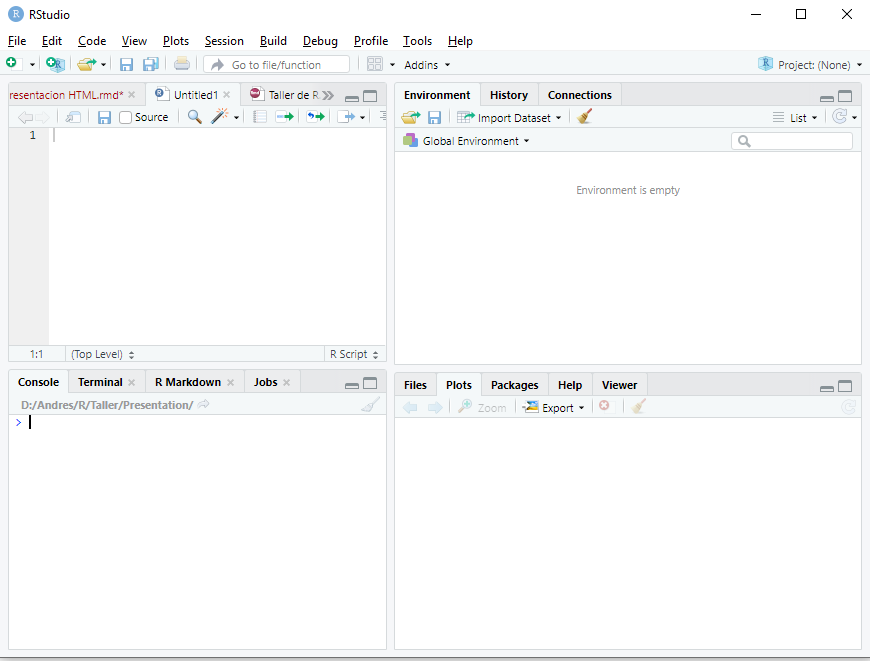
\includegraphics[keepaspectratio]{imgs/rstudio.png}}

\begin{enumerate}
\def\labelenumi{\arabic{enumi}.}
\item
  Ventana 1 - Script de trabajo: arriba a la izquierda. En ella
  abriremos y editaremos nuestros scripts de trabajo. A medida que se
  escriben las líneas para ejecutarlas debemos posicionarnos en ella (o
  seleccionarla) y correrlas (Run, arriba a la derecha, o más fácil
  \emph{Ctrl + r}).
\item
  Ventana 2 - consola: se ubica abajo a la izquierda. En ella se nos
  muestra el R propiamente dicho. Todo lo que nosotros ejecutamos en la
  ventana 1 se corre en esta segunda ventana, donde se nos muestra el
  resultado de nuestra corrida. Si se quiere se puede escribir
  directamente en ella, pero lo que hagamos no quedará guardado en
  nuestro script de trabajo.
\item
  Ventana 3 - objetos e historial: arriba a la derecha. Aquí podemos
  visualizar (en la pestaña \emph{Environment}) todos los objetos, bases
  de datos, funciones, etc. que hayamos importado o creado. Es muy
  importante ya que nos permite tener en vista nuestro entorno de
  trabajo (que es una funcionalidad con la que el R nativo no cuenta,
  uno debe memorizar los objetos creados). Si se tilda en alguno de los
  objetos, es equivalente a ejecutar el comando \texttt{View()}, y nos
  permite visualizar en forma de tabla nuestras bases de datos (se abren
  en la ventana 1). Contamos aquí con una opción gráfica para importar
  nuestras bases de datos, pero en este curso lo haremos directamente
  con código. También contamos con una escoba que nos permite borrar
  todos los objetos que tengamos. La segunda pestaña \emph{History} nos
  permite precisamente ver el historial de corridas que hayamos hecho.
  Allí podemos revisar comandos que ya ejecutamos y queremos repetir.
\item
  Ventana 4 - gráficos, paquetes y ayuda: abajo a la derecha. Usaremos 3
  de las pestañas:
\end{enumerate}

\begin{itemize}
\tightlist
\item
  \emph{Plots}: aquí visualizaremos todos los gráficos que vayamos
  generando. Nos permite mediante las flechas de arriba a la izquierda
  ir viendo también los gráficos anteriores. El icono Zoom nos facilita
  la visualización externa del gráfico que estemos viendo. Además
  presenta opciones de exportación.
\item
  \emph{Packages}: aquí podemos visualizar la lista completa de paquetes
  que tenemos instalados. Si tildamos uno lo activamos (equivalente al
  comando \texttt{library}, ver más adelante). Si tildamos en
  \emph{Install} podemos agregar nuevos paquetes que estén en el CRAN
  (base de datos de librerías).
\item
  \emph{Help}: como bien dice el nombre es la ventana de ayuda. Súper
  útil y de consulta constante. Allí podemos ver las descripciones que
  escribieron los creadores de cada función y/o paquete que usemos.
\end{itemize}

Como se ve RStudio nos permite realizar diversas acciones de forma
gráfica, sin necesidad de utilizar código. Mi postura en general es
dejar escrito en nuestro script la mayor cantidad de pasos posibles, ya
que todo lo que hagamos de forma gráfica no nos queda disponible cuando
volvamos a ver nuestro archivo. En este sentido, la instalación de
paquetes o las búsquedas de ayuda no es algo que necesitemos en un
futuro en nuestro script y podemos hacerlo de forma gráfica. Pero,
contrariamente, la carga de la base de datos, paquetes, exportación de
figuras, nos resultará de utilidad dejarlo plasmado en el escrito.

RStudio incluye un infinidad de opciones extra que no hacen al objetivo
de este curso. Para usos más avanzados es recomendable revisar la página
web de los creadores, que es muy completa e incluye muchas utilidades y
tutoriales. También se encuentra mucha ayuda en la pestaña Help.

\subsection{Script de trabajo}\label{script-de-trabajo}

En este apartado comenzaremos propiamente a desarrollar un script de
trabajo. Iremos viendo paso a paso como avanzar en su armado, desde la
carga de las librerías, introducir la base de datos y el manejo de la
misma, el análisis de los datos hasta la visualización gráfica de los
mismos.

Lo primero que hay que hacer un vez ingresados en RStudio es crear un
nuevo script (File -\textgreater{} New File -\textgreater{} R Script).
Allí nosotros podremos ir desarrollando los comandos correspondientes.

Todo script de trabajo tiene una estructura similar, la que yo utilizo
es:

\begin{itemize}
\tightlist
\item
  Carga de las librerías.
\item
  Carga de la base de datos.
\item
  Creación de las databases necesarias.
\item
  Armado de las funciones necesarias (si es que las tuviéramos).
\item
  Análisis de los datos separados por títulos.
\end{itemize}

Los títulos son marcas que hacemos para volver sencillamente a otras
partes de nuestro script (tengamos en cuenta que fácilmente se superan
las 1000 líneas). Para introducir un título (o marcador) colocamos la
palabra clave como un comentario y agregamos una serie de signos - a la
derecha. Por ejemplo:

\begin{Shaded}
\begin{Highlighting}[]
\CommentTok{\# Librerías {-}{-}{-}{-}{-}{-}}
\end{Highlighting}
\end{Shaded}

A partir de este momento podemos ver nuestros títulos en 2 lugares: en
la parte inferior izquierda de la ventana 1 o en la parte superior
derecha de la misma ventana en el icono con la leyenda \emph{Outline}.
Esta estructuración, insisto, es muy útil para movernos dentro del
documento sin perder mucho tiempo buscando algún comando. A su vez, si
introducimos más \# al comienzo, se generan títulos de un nivel
inferior.

\subsection{Instalación y carga de las
librerías}\label{instalaciuxf3n-y-carga-de-las-libreruxedas}

R se maneja en base a paquetes (o librerías) que contienen las funciones
que queramos utilizar. Como base R trae pre-instalados una serie de
paquetes que nos sirven para realizar gran cantidad de aplicaciones. Sin
embargo, es muy usual que prefiramos usar otras funciones no disponibles
en la base.

Para instalar una librería debemos ejecutar el código

\begin{Shaded}
\begin{Highlighting}[]
\FunctionTok{install.packages}\NormalTok{(}\StringTok{"nombre del paquete"}\NormalTok{)}
\end{Highlighting}
\end{Shaded}

La instalación de paquetes debemos realizarla una única vez. Como se
mencionó al describir la Ventana 4, también podemos instalar los
paquetes de un modo gráfico en la pestaña Packages de RStudio.

Cada vez que ingresamos a RStudio debemos cargar nuestras librerías a
utilizar. Para cargar una librería utilizamos el código

\begin{Shaded}
\begin{Highlighting}[]
\FunctionTok{library}\NormalTok{(}\StringTok{"nombre del paquete"}\NormalTok{)}
\end{Highlighting}
\end{Shaded}

Si queremos cargar varios paquetes, podemos ejecutar varios comandos
library en una misma línea separándolos con ``;'', y así cargar todos en
una única línea de corrida (Ctrl + r). Por otro lado, si bien uno puede
tener un conjunto de paquetes que utiliza habitualmente, no es
recomendable cargar de más ya que muchas veces se solapan funciones y
podemos tener alguna complicación.

Para el uso de este taller, instalaremos los paquetes
\textbf{agricolae}, \textbf{car}, \textbf{sciplot}, \textbf{patchwork},
\textbf{gridExtra} , \textbf{viridis} y \textbf{tidyverse}. Este último
incluye una serie de paquetes en su interior, que abarcan desde
funcionalidades gráficas hasta opciones del manejo de datos.

Así podemos cargarlos todos de la siguiente manera:

\begin{Shaded}
\begin{Highlighting}[]
\FunctionTok{library}\NormalTok{(agricolae);}\FunctionTok{library}\NormalTok{(tidyverse);}\FunctionTok{library}\NormalTok{(car)}
\FunctionTok{library}\NormalTok{(sciplot);}\FunctionTok{library}\NormalTok{(patchwork); }\FunctionTok{library}\NormalTok{(gridExtra)}
\end{Highlighting}
\end{Shaded}

\begin{verbatim}
## Warning: package 'patchwork' was built under R version 4.4.3
\end{verbatim}

\begin{Shaded}
\begin{Highlighting}[]
\FunctionTok{library}\NormalTok{(viridis)}
\end{Highlighting}
\end{Shaded}

\subsection{Carga de nuestros datos}\label{carga-de-nuestros-datos}

Como para casi cualquier acción que queramos ejecutar en R, la carga de
la base de datos puede hacerse de muchas maneras. En la ventana 3 se nos
ofrece una opción gráfica (a través de ``Import Dataset'').

De todas maneras, es recomendable hacerlo mediante código, para que cada
vez que ingresemos podamos incorporar la base de datos de manera muy
sencilla.

\subsubsection{Establecer el directorio de
trabajo}\label{establecer-el-directorio-de-trabajo}

Lo primero que debemos hacer es establecer el directorio de trabajo.
Para ello corremos el comando (con un directorio ejemplo):

\begin{Shaded}
\begin{Highlighting}[]
\FunctionTok{setwd}\NormalTok{(}\StringTok{"D:/DATOS/R"}\NormalTok{)}
\end{Highlighting}
\end{Shaded}

Si queremos revisar en qué directorio nos encontramos, ejecutamos

\begin{Shaded}
\begin{Highlighting}[]
\FunctionTok{getwd}\NormalTok{()}
\end{Highlighting}
\end{Shaded}

Ahora antes de ver cómo cargar la base de datos, haremos una breve
explicación de como crear la base de datos.

\subsubsection{Armado de la base de
datos}\label{armado-de-la-base-de-datos}

Una vez más, aquí mostraré mi forma de armar las bases de datos, hay
muchas\ldots{}

La forma de la base de datos es la misma que se utiliza en otros
software como Infostat. Debemos crear una columna por cada factor o
variable que tengamos, y repetir el nivel del factor para cada unidad
experimental (cada fila).

El formato en el que yo creo mis bases de datos es csv (archivo separado
por comas). Para ello se exporta desde Excel o Calc el archivo en ese
formato. El documento debe tener una única hoja con las base de datos
limpia, es decir sin columnas o filas extras con comentarios, datos
extra, etc. Por otro lado, es recomendable que los nombres de las
columnas sean lo más cortos posibles, y que no tengan espacios. Otra
recomendación es omitir el uso de tildes u otros caracteres especiales
en cualquier parte del documento puede llegar a tener problemas según la
codificación que usemos en RStudio. La más compatible es la UTF-8, que
no suele generar problemas.

Resumiendo, la recomendación es que una vez que tenemos nuestra tabla
(en Excel por ejemplo) con los datos listos, copiarla y pegarla en un
documento nuevo. Allí ver de simplificar los nombres de las columnas,
también de los niveles de factores a utilizar. Guardar este nuevo
documento como csv, si estamos en idioma español establecer para la
separación de columnas ``;''. Por supuesto, guardamos el archivo en el
directorio de trabajo.

Para este curso utilizaremos inicialmente la base de datos
``peces\_morfometria.csv''.

\subsubsection{Cargando la base de
datos}\label{cargando-la-base-de-datos}

R es un lenguaje orientado a objetos. Por lo tanto, cargaremos nuestra
base de datos como un ``objeto'' de R, al cual debemos asignarle un
nombre. De ahí en más, cualquier acción que modifique nuestro ``objeto''
quedará guardada en el objeto mismo, pero no modificará nuestro archivo
original (el csv en este caso). Para crear un objeto lo asignamos con
``\textbf{\textless-}'' (de forma rápida se escribe con \emph{Alt + -})
o con el signo ``\textbf{=}''.

Una primera forma de cargarla es mediante la función read.csv, y se
pueden establecer un par de parámetros:

\begin{Shaded}
\begin{Highlighting}[]
\NormalTok{datos\_peces }\OtherTok{\textless{}{-}} \FunctionTok{read.csv}\NormalTok{(}\StringTok{"data/peces\_morfometria.csv"}\NormalTok{, }\AttributeTok{dec=}\StringTok{"."}\NormalTok{, }\AttributeTok{sep=}\StringTok{","}\NormalTok{)}
\FunctionTok{lapply}\NormalTok{(datos\_peces, class) }\CommentTok{\# vemos que crea factores}
\end{Highlighting}
\end{Shaded}

\begin{verbatim}
## $id
## [1] "integer"
## 
## $especie
## [1] "character"
## 
## $sitio
## [1] "character"
## 
## $sexo
## [1] "character"
## 
## $temporada
## [1] "character"
## 
## $longitud_cm
## [1] "numeric"
## 
## $peso_g
## [1] "numeric"
## 
## $temperatura_C
## [1] "numeric"
## 
## $transparencia_cm
## [1] "integer"
## 
## $cortisol_ugdL
## [1] "numeric"
\end{verbatim}

La función que yo más utilizo es la que viene con el paquete
\textbf{tidyverse}, llamada \texttt{read\_csv}. Si usamos
\texttt{read\_csv2}, toma la coma como separador decimal:

\begin{Shaded}
\begin{Highlighting}[]
\NormalTok{datos\_peces }\OtherTok{\textless{}{-}} \FunctionTok{read\_csv}\NormalTok{(}\StringTok{"data/peces\_morfometria.csv"}\NormalTok{)}
\end{Highlighting}
\end{Shaded}

\begin{verbatim}
## Rows: 126 Columns: 10
## -- Column specification --------------------------------------------------------
## Delimiter: ","
## chr (4): especie, sitio, sexo, temporada
## dbl (6): id, longitud_cm, peso_g, temperatura_C, transparencia_cm, cortisol_...
## 
## i Use `spec()` to retrieve the full column specification for this data.
## i Specify the column types or set `show_col_types = FALSE` to quiet this message.
\end{verbatim}

Vemos que en este caso nos mostró directamente la clase de cada columna,
y que crea objetos tipo \emph{character} en vez de \emph{factor}.

En la ventana 3, nos aparecerán los objetos que incorporemos.

\subsection{Caracterización de la base de
datos}\label{caracterizaciuxf3n-de-la-base-de-datos}

Para ver los primeros 6 datos y los nombres de las columnas ejecutamos
la función \texttt{head}:

\begin{Shaded}
\begin{Highlighting}[]
\FunctionTok{head}\NormalTok{(datos\_peces)}
\end{Highlighting}
\end{Shaded}

\begin{verbatim}
## # A tibble: 6 x 10
##      id especie           sitio sexo  temporada longitud_cm peso_g temperatura_C
##   <dbl> <chr>             <chr> <chr> <chr>           <dbl>  <dbl>         <dbl>
## 1     1 Jenynsia multide~ Lagu~ F     Invierno          5.6   2.33          17.7
## 2     2 Odontesthes bona~ Lagu~ M     Verano           31.4 333.            21.7
## 3     3 Odontesthes bona~ Lagu~ M     Invierno         30.6 268.            15.7
## 4     4 Odontesthes bona~ Lagu~ M     Invierno         32.2 304.            20.4
## 5     5 Odontesthes bona~ Lagu~ F     Invierno         28.7 230.            20.5
## 6     6 Odontesthes bona~ Lagu~ F     Invierno         27.9 176.            16.8
## # i 2 more variables: transparencia_cm <dbl>, cortisol_ugdL <dbl>
\end{verbatim}

Para ver la tabla completa, se debe tildar en el nombre del objeto en la
ventana 3. Aprovechando que tenemos la tabla a nuestra vista, daré aquí
una breve descripción de los datos. Esta base de datos contiene
registros morfométricos, fisiológicos y ambientales de peces colectados
en tres lagunas pampeanas de la región central de Argentina. Se incluyen
tres especies nativas con rangos de talla muy distintos, lo que la hace
especialmente útil para explorar relaciones alométricas, correlaciones
entre variables continuas y comparaciones entre grupos. Las variables
registradas son:

\begin{itemize}
\item
  \textbf{id:} Identificador numérico único de cada individuo.
\item
  \textbf{especie:} Especie a la que pertenece el individuo
  (\emph{Odontesthes bonariensis}, \emph{Jenynsia multidentata} o
  \emph{Cichlasoma dimerus}).
\item
  \textbf{sitio:} Laguna de muestreo (Laguna Norte, Laguna Sur o Laguna
  Central).
\item
  \textbf{sexo:} Sexo del individuo (M/F).
\item
  \textbf{temporada:} Temporada de muestreo (Verano o Invierno).
\item
  \textbf{longitud\_cm:} Longitud total del pez en centímetros.
\item
  \textbf{peso\_g:} Peso corporal en gramos. Se relaciona con la
  longitud mediante una función alométrica (W = a·L\^{}b).
\item
  \textbf{temperatura\_C:} Temperatura del agua en el momento del
  muestreo, en °C.
\item
  \textbf{transparencia\_cm:} Transparencia del agua medida con disco de
  Secchi, en centímetros.
\item
  \textbf{cortisol\_ugdL:} Concentración plasmática de cortisol en
  µg/dL, utilizada como indicador de estrés fisiológico.
\end{itemize}

Siguiendo con el análisis de nuestra base de datos, podemos ver un
resumen de nuestra base o hacerle ``preguntas'' a R sobre la base de
datos. Al escribir ``\$'' a continuación de un objeto podemos ver las
columnas individuales. Por ejemplo:

\begin{Shaded}
\begin{Highlighting}[]
\FunctionTok{summary}\NormalTok{(datos\_peces) }\CommentTok{\# resumen de la base}
\end{Highlighting}
\end{Shaded}

\begin{verbatim}
##        id           especie             sitio               sexo          
##  Min.   :  1.00   Length:126         Length:126         Length:126        
##  1st Qu.: 32.25   Class :character   Class :character   Class :character  
##  Median : 63.50   Mode  :character   Mode  :character   Mode  :character  
##  Mean   : 63.50                                                           
##  3rd Qu.: 94.75                                                           
##  Max.   :126.00                                                           
##   temporada          longitud_cm        peso_g        temperatura_C  
##  Length:126         Min.   : 4.10   Min.   :  0.810   Min.   :14.90  
##  Class :character   1st Qu.: 6.30   1st Qu.:  2.835   1st Qu.:18.20  
##  Mode  :character   Median :11.85   Median : 15.810   Median :19.75  
##                     Mean   :15.33   Mean   : 84.457   Mean   :19.78  
##                     3rd Qu.:26.48   3rd Qu.:150.458   3rd Qu.:21.30  
##                     Max.   :36.20   Max.   :518.570   Max.   :24.40  
##  transparencia_cm cortisol_ugdL  
##  Min.   :11.00    Min.   :0.500  
##  1st Qu.:36.00    1st Qu.:2.333  
##  Median :43.50    Median :3.650  
##  Mean   :44.12    Mean   :3.719  
##  3rd Qu.:51.75    3rd Qu.:5.003  
##  Max.   :74.00    Max.   :7.950
\end{verbatim}

\begin{Shaded}
\begin{Highlighting}[]
\FunctionTok{is.double}\NormalTok{(datos\_peces}\SpecialCharTok{$}\NormalTok{temperatura\_C) }\CommentTok{\# double indica numérico continuo}
\end{Highlighting}
\end{Shaded}

\begin{verbatim}
## [1] TRUE
\end{verbatim}

\begin{Shaded}
\begin{Highlighting}[]
\FunctionTok{is.character}\NormalTok{(datos\_peces}\SpecialCharTok{$}\NormalTok{longitud\_cm)}
\end{Highlighting}
\end{Shaded}

\begin{verbatim}
## [1] FALSE
\end{verbatim}

\begin{Shaded}
\begin{Highlighting}[]
\FunctionTok{levels}\NormalTok{(}\FunctionTok{as.factor}\NormalTok{(datos\_peces}\SpecialCharTok{$}\NormalTok{especie)) }\CommentTok{\# para ver los niveles de un factor}
\end{Highlighting}
\end{Shaded}

\begin{verbatim}
## [1] "Cichlasoma dimerus"      "Jenynsia multidentata"  
## [3] "Odontesthes bonariensis"
\end{verbatim}

\begin{Shaded}
\begin{Highlighting}[]
\FunctionTok{as.character}\NormalTok{(datos\_peces}\SpecialCharTok{$}\NormalTok{transparencia\_cm)}
\end{Highlighting}
\end{Shaded}

\begin{verbatim}
##   [1] "48" "40" "47" "33" "34" "38" "35" "36" "41" "30" "42" "49" "16" "46" "34"
##  [16] "30" "27" "33" "34" "47" "28" "56" "33" "51" "56" "28" "56" "70" "38" "51"
##  [31] "42" "45" "42" "38" "53" "55" "44" "63" "58" "53" "36" "67" "61" "19" "31"
##  [46] "39" "56" "60" "41" "48" "53" "30" "52" "41" "47" "44" "31" "33" "45" "47"
##  [61] "42" "58" "41" "30" "41" "43" "43" "59" "51" "58" "52" "43" "57" "42" "48"
##  [76] "33" "46" "41" "50" "67" "74" "57" "45" "55" "48" "38" "44" "42" "38" "62"
##  [91] "39" "39" "54" "37" "31" "35" "51" "50" "49" "40" "34" "56" "28" "43" "29"
## [106] "40" "43" "60" "11" "62" "35" "49" "55" "36" "44" "51" "44" "36" "48" "47"
## [121] "27" "62" "48" "16" "35" "66"
\end{verbatim}

\subsubsection{Caracterización
gráfica}\label{caracterizaciuxf3n-gruxe1fica}

En este caso haremos algunos gráficos sencillos para observar la
distribución de nuestra base de datos. La función \texttt{plot} (y sus
derivados, como en este caso \texttt{boxplot}) viene con R base y es la
forma más rápida y sencilla de graficar.

\begin{Shaded}
\begin{Highlighting}[]
\FunctionTok{plot}\NormalTok{(datos\_peces}\SpecialCharTok{$}\NormalTok{longitud\_cm)}
\end{Highlighting}
\end{Shaded}


\includegraphics[width=0.5\linewidth]{curso_2026_markdown_files/figure-latex/unnamed-chunk-10-1}

\begin{Shaded}
\begin{Highlighting}[]
\FunctionTok{plot}\NormalTok{(datos\_peces}\SpecialCharTok{$}\NormalTok{longitud\_cm}\SpecialCharTok{\textasciitilde{}}\NormalTok{datos\_peces}\SpecialCharTok{$}\NormalTok{temperatura\_C)}
\end{Highlighting}
\end{Shaded}


\includegraphics[width=0.5\linewidth]{curso_2026_markdown_files/figure-latex/unnamed-chunk-10-2}

\begin{Shaded}
\begin{Highlighting}[]
\FunctionTok{boxplot}\NormalTok{(datos\_peces}\SpecialCharTok{$}\NormalTok{peso\_g}\SpecialCharTok{\textasciitilde{}}\NormalTok{datos\_peces}\SpecialCharTok{$}\NormalTok{especie)}
\end{Highlighting}
\end{Shaded}


\includegraphics[width=0.5\linewidth]{curso_2026_markdown_files/figure-latex/unnamed-chunk-10-3}

\begin{Shaded}
\begin{Highlighting}[]
\FunctionTok{boxplot}\NormalTok{(datos\_peces}\SpecialCharTok{$}\NormalTok{peso\_g}\SpecialCharTok{\textasciitilde{}}\NormalTok{datos\_peces}\SpecialCharTok{$}\NormalTok{sitio)}
\end{Highlighting}
\end{Shaded}


\includegraphics[width=0.5\linewidth]{curso_2026_markdown_files/figure-latex/unnamed-chunk-10-4}

\subsection{Manejo de la base de
datos}\label{manejo-de-la-base-de-datos}

\subsubsection{Subdividir la base de
datos}\label{subdividir-la-base-de-datos}

Algo muy común en el trabajo en R, es la necesidad de subdividir la base
de datos para utilizar únicamente una parte de ella. Veremos un par de
formas de hacerlo.

Con las funciones que incluye R base, utilizaremos \texttt{subset}. Por
ejemplo para elegir solo las muestras de la especie \emph{Jenynsia
multidentata}:

\begin{Shaded}
\begin{Highlighting}[]
\NormalTok{JENYNSIA }\OtherTok{\textless{}{-}} \FunctionTok{subset}\NormalTok{(datos\_peces, datos\_peces}\SpecialCharTok{$}\NormalTok{especie }\SpecialCharTok{==} \StringTok{"Jenynsia multidentata"}\NormalTok{)}
\end{Highlighting}
\end{Shaded}

Y creamos un objeto que se llama \emph{JENYNSIA}, nuevamente mediante
\emph{\textless-}.

Otra forma de hacerlo es mediante el uso de pipes
(\textbf{\%\textgreater\%}). Las pipes sirven para concatenar una serie
de acciones para modificar una base de datos. En primer lugar se ubica
la base a modificar y entre cada linea de comando \%\textgreater\%
(\emph{Ctrl + Shift + m}). Así, podemos filtrar una base de datos con
\texttt{filter}:

\begin{Shaded}
\begin{Highlighting}[]
\NormalTok{Laguna\_Central }\OtherTok{\textless{}{-}}\NormalTok{ datos\_peces }\SpecialCharTok{\%\textgreater{}\%} \FunctionTok{filter}\NormalTok{(sitio }\SpecialCharTok{==} \StringTok{"Laguna Central"}\NormalTok{)}
\end{Highlighting}
\end{Shaded}

Si queremos filtrar por más de un parámetro:

\begin{Shaded}
\begin{Highlighting}[]
\CommentTok{\# en dos pasos}
\NormalTok{Peces\_Invierno }\OtherTok{\textless{}{-}}\NormalTok{ datos\_peces }\SpecialCharTok{\%\textgreater{}\%} 
  \FunctionTok{filter}\NormalTok{(temporada }\SpecialCharTok{==} \StringTok{"Invierno"}\NormalTok{) }\SpecialCharTok{\%\textgreater{}\%} \CommentTok{\# se agrega a lo anterior}
  \FunctionTok{filter}\NormalTok{(especie }\SpecialCharTok{==} \StringTok{"Cichlasoma dimerus"} \SpecialCharTok{|}\NormalTok{ especie }\SpecialCharTok{==} \StringTok{"Odontesthes bonariensis"}\NormalTok{)}
\end{Highlighting}
\end{Shaded}

\subsubsection{Seleccionar filas o
columnas}\label{seleccionar-filas-o-columnas}

En R base, el uso de \[ \] sirve para seleccionar filas o columnas de
una database, tal que \texttt{data{[}filas,columnas{]}}. En el entorno
de \emph{dplyr} utilizaremos la función \texttt{select} para columnas:

\begin{Shaded}
\begin{Highlighting}[]
\CommentTok{\# seleccionar filas 1 a 3}
\NormalTok{datos\_peces[}\DecValTok{1}\SpecialCharTok{:}\DecValTok{3}\NormalTok{,]}
\end{Highlighting}
\end{Shaded}

\begin{verbatim}
## # A tibble: 3 x 10
##      id especie           sitio sexo  temporada longitud_cm peso_g temperatura_C
##   <dbl> <chr>             <chr> <chr> <chr>           <dbl>  <dbl>         <dbl>
## 1     1 Jenynsia multide~ Lagu~ F     Invierno          5.6   2.33          17.7
## 2     2 Odontesthes bona~ Lagu~ M     Verano           31.4 333.            21.7
## 3     3 Odontesthes bona~ Lagu~ M     Invierno         30.6 268.            15.7
## # i 2 more variables: transparencia_cm <dbl>, cortisol_ugdL <dbl>
\end{verbatim}

\begin{Shaded}
\begin{Highlighting}[]
\CommentTok{\# seleccionar columnas 1 a 3}
\NormalTok{datos\_peces[,}\DecValTok{1}\SpecialCharTok{:}\DecValTok{3}\NormalTok{]}
\end{Highlighting}
\end{Shaded}

\begin{verbatim}
## # A tibble: 126 x 3
##       id especie                 sitio         
##    <dbl> <chr>                   <chr>         
##  1     1 Jenynsia multidentata   Laguna Central
##  2     2 Odontesthes bonariensis Laguna Central
##  3     3 Odontesthes bonariensis Laguna Norte  
##  4     4 Odontesthes bonariensis Laguna Central
##  5     5 Odontesthes bonariensis Laguna Sur    
##  6     6 Odontesthes bonariensis Laguna Norte  
##  7     7 Cichlasoma dimerus      Laguna Norte  
##  8     8 Odontesthes bonariensis Laguna Central
##  9     9 Odontesthes bonariensis Laguna Sur    
## 10    10 Odontesthes bonariensis Laguna Central
## # i 116 more rows
\end{verbatim}

\begin{Shaded}
\begin{Highlighting}[]
\NormalTok{datos\_peces }\SpecialCharTok{\%\textgreater{}\%} \FunctionTok{select}\NormalTok{(}\DecValTok{1}\SpecialCharTok{:}\DecValTok{3}\NormalTok{)}
\end{Highlighting}
\end{Shaded}

\begin{verbatim}
## # A tibble: 126 x 3
##       id especie                 sitio         
##    <dbl> <chr>                   <chr>         
##  1     1 Jenynsia multidentata   Laguna Central
##  2     2 Odontesthes bonariensis Laguna Central
##  3     3 Odontesthes bonariensis Laguna Norte  
##  4     4 Odontesthes bonariensis Laguna Central
##  5     5 Odontesthes bonariensis Laguna Sur    
##  6     6 Odontesthes bonariensis Laguna Norte  
##  7     7 Cichlasoma dimerus      Laguna Norte  
##  8     8 Odontesthes bonariensis Laguna Central
##  9     9 Odontesthes bonariensis Laguna Sur    
## 10    10 Odontesthes bonariensis Laguna Central
## # i 116 more rows
\end{verbatim}

\begin{Shaded}
\begin{Highlighting}[]
\CommentTok{\# seleccionar por nombre de la columna}
\NormalTok{datos\_peces }\SpecialCharTok{\%\textgreater{}\%} \FunctionTok{select}\NormalTok{(sitio, especie)}
\end{Highlighting}
\end{Shaded}

\begin{verbatim}
## # A tibble: 126 x 2
##    sitio          especie                
##    <chr>          <chr>                  
##  1 Laguna Central Jenynsia multidentata  
##  2 Laguna Central Odontesthes bonariensis
##  3 Laguna Norte   Odontesthes bonariensis
##  4 Laguna Central Odontesthes bonariensis
##  5 Laguna Sur     Odontesthes bonariensis
##  6 Laguna Norte   Odontesthes bonariensis
##  7 Laguna Norte   Cichlasoma dimerus     
##  8 Laguna Central Odontesthes bonariensis
##  9 Laguna Sur     Odontesthes bonariensis
## 10 Laguna Central Odontesthes bonariensis
## # i 116 more rows
\end{verbatim}

\subsubsection{Creación de nuevas
variables}\label{creaciuxf3n-de-nuevas-variables}

Una opción muy útil ligada al paquete \textbf{dplyr} es la de
transformar nuestras bases de datos para algún gráfico en particular,
sin necesidad de cambiar la tabla original. Para ello utilizaremos la
función \texttt{mutate}, que permite generar muchos cambios en la base
de datos. Por ejemplo, en la base \texttt{datos\_peces}, si queremos
agregar la la variable peso por unidad de longitud:

\begin{Shaded}
\begin{Highlighting}[]
\NormalTok{datos\_peces }\OtherTok{\textless{}{-}}\NormalTok{ datos\_peces }\SpecialCharTok{\%\textgreater{}\%} 
  \FunctionTok{mutate}\NormalTok{(}\StringTok{"peso\_relativo"} \OtherTok{=}\NormalTok{ peso\_g}\SpecialCharTok{/}\NormalTok{longitud\_cm) }\CommentTok{\# se crea una nueva columna}

\CommentTok{\# para ver la columna nueva}
\FunctionTok{head}\NormalTok{(datos\_peces}\SpecialCharTok{$}\NormalTok{peso\_relativo)}
\end{Highlighting}
\end{Shaded}

\begin{verbatim}
## [1]  0.4160714 10.6140127  8.7584967  9.4360248  8.0087108  6.3043011
\end{verbatim}

\subsubsection{Cambio en los niveles de un
factor}\label{cambio-en-los-niveles-de-un-factor}

También podemos cambiar los niveles de una factor \texttt{mutate},
mediante la siguiente estructura:

\begin{Shaded}
\begin{Highlighting}[]
\NormalTok{... }\SpecialCharTok{\%\textgreater{}\%}
  \FunctionTok{mutate}\NormalTok{(}\AttributeTok{nombre\_factor =} \FunctionTok{fct\_recode}\NormalTok{(nombre\_factor,}
                        \StringTok{"nombre nuevo"} \OtherTok{=} \StringTok{"nombre viejo"}\NormalTok{))}
\end{Highlighting}
\end{Shaded}

Y podemos incluir una línea para cada nivel que queramos modificar. Por
ejemplo:

\begin{Shaded}
\begin{Highlighting}[]
\NormalTok{datos\_peces }\OtherTok{\textless{}{-}}\NormalTok{ datos\_peces }\SpecialCharTok{\%\textgreater{}\%} 
  \FunctionTok{mutate}\NormalTok{(}\AttributeTok{sexo =} \FunctionTok{fct\_recode}\NormalTok{(sexo,}
                           \StringTok{"Macho"} \OtherTok{=} \StringTok{"M"}\NormalTok{,}
                           \StringTok{"Hembra"} \OtherTok{=} \StringTok{"F"}\NormalTok{))}
\end{Highlighting}
\end{Shaded}

\subsection{Actividad 1}\label{actividad-1}

\begin{enumerate}
\def\labelenumi{\arabic{enumi}.}
\tightlist
\item
  Cree a partir de la base de datos original, una que contenga
  únicamente los individuos de la especie \emph{Cichlasoma dimerus y
  Odontesthes bonariensis} que se encuentran en la Laguna Norte en
  invierno.
\item
  Filtre la base creada para obtener otra que solo tenga aquellos
  individuos con peso relativo mayor a 1.
\end{enumerate}

\section{Unidad 2. Análisis y representación de datos
numéricos}\label{unidad-2.-anuxe1lisis-y-representaciuxf3n-de-datos-numuxe9ricos}

Veremos los análisis a realizar para procesar variables continuas
(correlación y regresión) y como representarlas gráficamente de una
forma más detallada que como lo vimos hasta ahora.

\subsection{Correlación}\label{correlaciuxf3n}

Cuando queremos evaluar la relación entre 2 variables continuas, sin
establecer relaciones de dependencia, el análisis que debemos hacer es
un análisis de correlación lineal. El test de correlación lineal más
utilizado es el de correlación de Pearson, que nos arroja el coeficiente
de Pearson, que toma valores entre -1 y 1, según la relación sea inversa
o directa. Valores cercanos a cero indican falta de relación entre las
variables. La correlación de Pearson tiene como supuestos la
distribución normal de las variables (entre otros). Debemos poner a
prueba esos supuestos para poder realizar este tipo de análisis.

Comenzaremos creando una base de datos de los individuos de
\emph{Odontesthes bonariensis}:

\begin{Shaded}
\begin{Highlighting}[]
\NormalTok{PEJERREY }\OtherTok{\textless{}{-}}\NormalTok{ datos\_peces }\SpecialCharTok{\%\textgreater{}\%} \FunctionTok{filter}\NormalTok{(especie }\SpecialCharTok{==} \StringTok{"Odontesthes bonariensis"}\NormalTok{)}
\end{Highlighting}
\end{Shaded}

Veremos primero como analizar de a pares de variables. Lo recomendable
es iniciar con una exploración gráfica de los datos, en este caso vamos
a relacionar la longitud con el peso de los individuos.

\begin{Shaded}
\begin{Highlighting}[]
\CommentTok{\# Exploración gráfica}

\FunctionTok{plot}\NormalTok{(PEJERREY}\SpecialCharTok{$}\NormalTok{longitud\_cm, }\AttributeTok{pch =} \DecValTok{19}\NormalTok{)}
\end{Highlighting}
\end{Shaded}


\includegraphics[width=0.5\linewidth]{curso_2026_markdown_files/figure-latex/unnamed-chunk-19-1}

\begin{Shaded}
\begin{Highlighting}[]
\FunctionTok{plot}\NormalTok{(PEJERREY}\SpecialCharTok{$}\NormalTok{peso\_g, }\AttributeTok{pch =} \DecValTok{17}\NormalTok{)}
\end{Highlighting}
\end{Shaded}


\includegraphics[width=0.5\linewidth]{curso_2026_markdown_files/figure-latex/unnamed-chunk-19-2}

\begin{Shaded}
\begin{Highlighting}[]
\FunctionTok{plot}\NormalTok{(PEJERREY}\SpecialCharTok{$}\NormalTok{longitud\_cm, PEJERREY}\SpecialCharTok{$}\NormalTok{peso\_g)}
\end{Highlighting}
\end{Shaded}


\includegraphics[width=0.5\linewidth]{curso_2026_markdown_files/figure-latex/unnamed-chunk-19-3}

\begin{Shaded}
\begin{Highlighting}[]
\FunctionTok{plot}\NormalTok{(PEJERREY}\SpecialCharTok{$}\NormalTok{longitud\_cm)}
\end{Highlighting}
\end{Shaded}


\includegraphics[width=0.5\linewidth]{curso_2026_markdown_files/figure-latex/unnamed-chunk-19-4}

Ahora veremos cómo hacer la correlación de pearson, de momento ignorando
los supuestos:

\begin{Shaded}
\begin{Highlighting}[]
\FunctionTok{cor.test}\NormalTok{(PEJERREY}\SpecialCharTok{$}\NormalTok{longitud\_cm, PEJERREY}\SpecialCharTok{$}\NormalTok{peso\_g, }\AttributeTok{method =} \StringTok{"pearson"}\NormalTok{)}
\end{Highlighting}
\end{Shaded}

\begin{verbatim}
## 
##  Pearson's product-moment correlation
## 
## data:  PEJERREY$longitud_cm and PEJERREY$peso_g
## t = 16.507, df = 40, p-value < 2.2e-16
## alternative hypothesis: true correlation is not equal to 0
## 95 percent confidence interval:
##  0.8794780 0.9641087
## sample estimates:
##       cor 
## 0.9338029
\end{verbatim}

Vemos que nos arroja los resultados del valor del coeficiente lineal de
pearson y su valor p asociado.

\subsubsection{Análisis de normalidad}\label{anuxe1lisis-de-normalidad}

En esta sección veremos cómo poner a prueba la normalidad de nuestros
datos con el test de Shapiro Wilk y como visualizarlo gráficamente en un
qqplot. Recordemos que la hipótesis nula del test es que los datos son
normales, por lo que si rechazamos la hipótesis (p\textless0,05) no hay
normalidad:

\begin{Shaded}
\begin{Highlighting}[]
\CommentTok{\# Forma analítica}

\FunctionTok{shapiro.test}\NormalTok{(PEJERREY}\SpecialCharTok{$}\NormalTok{longitud\_cm)}
\end{Highlighting}
\end{Shaded}

\begin{verbatim}
## 
##  Shapiro-Wilk normality test
## 
## data:  PEJERREY$longitud_cm
## W = 0.96648, p-value = 0.2504
\end{verbatim}

\begin{Shaded}
\begin{Highlighting}[]
\FunctionTok{shapiro.test}\NormalTok{(PEJERREY}\SpecialCharTok{$}\NormalTok{peso\_g)}
\end{Highlighting}
\end{Shaded}

\begin{verbatim}
## 
##  Shapiro-Wilk normality test
## 
## data:  PEJERREY$peso_g
## W = 0.97219, p-value = 0.39
\end{verbatim}

\begin{Shaded}
\begin{Highlighting}[]
\CommentTok{\# Forma gráfica}
\FunctionTok{qqnorm}\NormalTok{(PEJERREY}\SpecialCharTok{$}\NormalTok{longitud\_cm)}
\FunctionTok{qqline}\NormalTok{(PEJERREY}\SpecialCharTok{$}\NormalTok{longitud\_cm, }\AttributeTok{col=}\StringTok{"red"}\NormalTok{, }\AttributeTok{lwd=}\DecValTok{2}\NormalTok{)}

\FunctionTok{qqnorm}\NormalTok{(PEJERREY}\SpecialCharTok{$}\NormalTok{peso\_g)}
\FunctionTok{qqline}\NormalTok{(PEJERREY}\SpecialCharTok{$}\NormalTok{peso\_g, }\AttributeTok{col=}\StringTok{"red"}\NormalTok{, }\AttributeTok{lwd=}\DecValTok{2}\NormalTok{)}
\end{Highlighting}
\end{Shaded}


\includegraphics[width=0.5\linewidth]{curso_2026_markdown_files/figure-latex/unnamed-chunk-21-1}

\includegraphics[width=0.5\linewidth]{curso_2026_markdown_files/figure-latex/unnamed-chunk-21-2}

Vemos que para ambos casos las variable presentan un comportamiento
normal de acuerdo al test analítico y al gráfico.

Si quisiéramos hacer una transformación de nuestros datos, en R lo
podemos hacer directamente:

\begin{Shaded}
\begin{Highlighting}[]
\FunctionTok{shapiro.test}\NormalTok{(}\FunctionTok{log}\NormalTok{(PEJERREY}\SpecialCharTok{$}\NormalTok{peso\_g}\SpecialCharTok{+}\DecValTok{1}\NormalTok{)) }\CommentTok{\# convertimos al logaritmo en base 10}

\FunctionTok{qqnorm}\NormalTok{(}\FunctionTok{log}\NormalTok{(PEJERREY}\SpecialCharTok{$}\NormalTok{peso\_g}\SpecialCharTok{+}\DecValTok{1}\NormalTok{))}
\FunctionTok{qqline}\NormalTok{(}\FunctionTok{log}\NormalTok{(PEJERREY}\SpecialCharTok{$}\NormalTok{peso\_g}\SpecialCharTok{+}\DecValTok{1}\NormalTok{), }\AttributeTok{col=}\StringTok{"red"}\NormalTok{, }\AttributeTok{lwd=}\DecValTok{2}\NormalTok{)}
\end{Highlighting}
\end{Shaded}

Si no logramos de ninguna manera corregir la normalidad, podemos también
correr el test no paramétrico de Spearman que no tiene supuestos
asociados, aunque también presenta menor potencia. En este caso el
coeficiente es el coeficiente de Spearman (\emph{rho}):

\begin{Shaded}
\begin{Highlighting}[]
\FunctionTok{cor.test}\NormalTok{(PEJERREY}\SpecialCharTok{$}\NormalTok{longitud\_cm, PEJERREY}\SpecialCharTok{$}\NormalTok{peso\_g, }
        \AttributeTok{method =} \StringTok{"spearman"}\NormalTok{, }\AttributeTok{exact =} \ConstantTok{TRUE}\NormalTok{)}
\end{Highlighting}
\end{Shaded}

\begin{verbatim}
## 
##  Spearman's rank correlation rho
## 
## data:  PEJERREY$longitud_cm and PEJERREY$peso_g
## S = 482.68, p-value < 2.2e-16
## alternative hypothesis: true rho is not equal to 0
## sample estimates:
##       rho 
## 0.9608885
\end{verbatim}

\subsubsection{Muchas columnas a la vez}\label{muchas-columnas-a-la-vez}

Existen otros test que permiten correlacionar pares de variables pero
correrlas todas a la vez. A diferencia de la función \texttt{cor.test}
que solo admite 2 variables, la función \texttt{cor} permite cargar una
serie de columnas y luego podemos ver los coeficientes en forma
matricial:

\begin{Shaded}
\begin{Highlighting}[]
\NormalTok{CORR }\OtherTok{\textless{}{-}} \FunctionTok{cor}\NormalTok{(PEJERREY[, }\FunctionTok{c}\NormalTok{(}\StringTok{"longitud\_cm"}\NormalTok{, }\StringTok{"peso\_g"}\NormalTok{, }\StringTok{"temperatura\_C"}\NormalTok{, }\StringTok{"transparencia\_cm"}\NormalTok{)],}
            \AttributeTok{method =} \StringTok{"pearson"}\NormalTok{)}
\NormalTok{CORR }\CommentTok{\# obtenemos los coeficientes}
\end{Highlighting}
\end{Shaded}

\begin{verbatim}
##                  longitud_cm      peso_g temperatura_C transparencia_cm
## longitud_cm       1.00000000  0.93380294   -0.16328425       0.03128702
## peso_g            0.93380294  1.00000000   -0.11177907       0.04206695
## temperatura_C    -0.16328425 -0.11177907    1.00000000      -0.06799808
## transparencia_cm  0.03128702  0.04206695   -0.06799808       1.00000000
\end{verbatim}

Otra función de utilidad que nos permite ver los coeficientes y los
valores \emph{p} al mismo tiempo es la función \texttt{rcorr} del
paquete \textbf{Hmisc}:

\begin{Shaded}
\begin{Highlighting}[]
\FunctionTok{library}\NormalTok{(Hmisc)}
\NormalTok{CORR\_Pejerrey }\OtherTok{\textless{}{-}} \FunctionTok{rcorr}\NormalTok{(}\FunctionTok{as.matrix}\NormalTok{(PEJERREY[,}\DecValTok{6}\SpecialCharTok{:}\DecValTok{9}\NormalTok{]))}
\NormalTok{CORR\_Pejerrey }\CommentTok{\# aquí observamos primero los valores de coeficientes y luego el valor p}
\end{Highlighting}
\end{Shaded}

\begin{verbatim}
##                  longitud_cm peso_g temperatura_C transparencia_cm
## longitud_cm             1.00   0.93         -0.16             0.03
## peso_g                  0.93   1.00         -0.11             0.04
## temperatura_C          -0.16  -0.11          1.00            -0.07
## transparencia_cm        0.03   0.04         -0.07             1.00
## 
## n= 42 
## 
## 
## P
##                  longitud_cm peso_g temperatura_C transparencia_cm
## longitud_cm                  0.0000 0.3015        0.8441          
## peso_g           0.0000             0.4810        0.7914          
## temperatura_C    0.3015      0.4810               0.6687          
## transparencia_cm 0.8441      0.7914 0.6687
\end{verbatim}

Ahora veremos dos paquetes que nos permiten ver en forma gráfica el
resultado de nuestra correlación. El primero es el paquete
\textbf{corrplot} del cual usaremos las funciones \texttt{cor.mtest} y
\texttt{corrplot}:

\begin{Shaded}
\begin{Highlighting}[]
\FunctionTok{library}\NormalTok{(corrplot)}
\FunctionTok{corrplot}\NormalTok{(CORR\_Pejerrey}\SpecialCharTok{$}\NormalTok{r)}
\end{Highlighting}
\end{Shaded}

\begin{center}
\includegraphics{curso_2026_markdown_files/figure-latex/unnamed-chunk-26-1} \end{center}

\begin{Shaded}
\begin{Highlighting}[]
\FunctionTok{corrplot}\NormalTok{(CORR\_Pejerrey}\SpecialCharTok{$}\NormalTok{r, }
         \AttributeTok{type =} \StringTok{"upper"}\NormalTok{,  }\CommentTok{\# solo mitad de arriba }
         \AttributeTok{tl.col =} \StringTok{"black"}\NormalTok{,  }\CommentTok{\# color letras}
         \AttributeTok{addCoef.col =} \StringTok{\textquotesingle{}grey20\textquotesingle{}}\NormalTok{, }\CommentTok{\# color números}
         \AttributeTok{p.mat =}\NormalTok{ CORR\_Pejerrey}\SpecialCharTok{$}\NormalTok{P, }\CommentTok{\# valores p}
         \AttributeTok{sig.level =} \FloatTok{0.05}\NormalTok{,  }
         \AttributeTok{insig =} \StringTok{\textquotesingle{}blank\textquotesingle{}}\NormalTok{,   }\CommentTok{\# qué hacer con los no significativos}
         \AttributeTok{tl.srt =} \DecValTok{45}\NormalTok{,     }\CommentTok{\# ángulo de títulos}
         \AttributeTok{diag =} \ConstantTok{FALSE}\NormalTok{)}
\end{Highlighting}
\end{Shaded}

\begin{center}
\includegraphics{curso_2026_markdown_files/figure-latex/unnamed-chunk-26-2} \end{center}

Finalmente, introduciré la función \texttt{chart.Correlation} del
paquete \textbf{PerformanceAnalytics}, que permite visualizar
interacciones, gráficos de dispersión, coeficientes de correlación y
significancia todo al mismo tiempo:

\begin{Shaded}
\begin{Highlighting}[]
\FunctionTok{library}\NormalTok{(}\StringTok{"PerformanceAnalytics"}\NormalTok{)}
\FunctionTok{chart.Correlation}\NormalTok{(PEJERREY[,}\DecValTok{6}\SpecialCharTok{:}\DecValTok{8}\NormalTok{], }
                  \AttributeTok{histogram=}\ConstantTok{TRUE}\NormalTok{, }
                  \AttributeTok{method =} \StringTok{"pearson"}\NormalTok{,}
                  \AttributeTok{pch=}\DecValTok{19}\NormalTok{)}
\end{Highlighting}
\end{Shaded}

\pandocbounded{
\includegraphics[keepaspectratio]{curso_2026_markdown_files/figure-latex/unnamed-chunk-27-1.pdf}}

Los invito a profundizar más en el uso de los paquetes por su propia
cuenta.

\subsubsection{Actividad 2.a}\label{actividad-2.a}

Genere bases de datos para cada una de las especies y analice si existe
una correlación entre longitud\_cm, peso\_g, cortisol en sangre,
temperatura y transparencia. Realice un gráfico con corrplot y otro con
chart.Correlation, explore posibilidades de las funciones en la sección
ayuda.

\subsection{Regresión lineal simple}\label{regresiuxf3n-lineal-simple}

El análisis de regresión lineal tiene algunos parecidos con el de
correlación, pero en este caso hay una de la variables que consideramos
que influye en la otra. Es decir, que hay una variable \emph{x}
independiente (regresora) y una \emph{y} dependiente. Ambas variables
deben ser numéricas. El modelo plantea el ajuste lineal de los datos,
por lo tanto hay pruebas de hipótesis para la ordenada al origen y la
pendiente de la recta de ajuste. Los supuestos del modelo son la
distribución normal de las variables y la homogeneidad de los errores.
Un detalle importante, es que el modelo solo es válido en el rango de
nuestra \emph{x}.

Por otro lado, existe un parámetro llamado el coeficiente de
determinación (R\textsuperscript{2}) que nos da una idea de qué
porcentaje de variabilidad de \emph{y} está siendo explicado con
\emph{x}. Este coeficiente toma valores entre 0 y 1, cuanto mayor es
mejor es el ajuste de nuestra nube de puntos a la recta.

Para analizar una regresión lineal en nuestra base datos, retomaremos la
relación entre largo y peso de los peces, aunque en este caso
entendiendo que el peso depende del largo del pez. Así por ejemplo, para
la especie \emph{Jenynsia multidentata}:

\begin{Shaded}
\begin{Highlighting}[]
\FunctionTok{plot}\NormalTok{(JENYNSIA}\SpecialCharTok{$}\NormalTok{longitud\_cm, JENYNSIA}\SpecialCharTok{$}\NormalTok{peso\_g, }\AttributeTok{pch=}\DecValTok{19}\NormalTok{)}
\end{Highlighting}
\end{Shaded}

\begin{center}
\includegraphics[width=0.6\linewidth]{curso_2026_markdown_files/figure-latex/unnamed-chunk-28-1} \end{center}

Para realizar una regresión lineal (y que en realidad será de la misma
manera para un ANOVA), se debe plantear un modelo lineal mediante la
función \texttt{lm} de la forma \texttt{lm(y\textasciitilde{}x)}:

\begin{Shaded}
\begin{Highlighting}[]
\NormalTok{fit\_Jenysia }\OtherTok{\textless{}{-}}\FunctionTok{lm}\NormalTok{(peso\_g }\SpecialCharTok{\textasciitilde{}}\NormalTok{ longitud\_cm, }\AttributeTok{data =}\NormalTok{ JENYNSIA)}
\end{Highlighting}
\end{Shaded}

Una vez creado el objeto, vamos a poner a prueba los supuestos, tanto de
forma gráfica como analítica. Al someter nuestro modelo a la función
\texttt{plot}, se nos crean 4 gráficos para poner a prueba los
supuestos. Para verlos todos juntos dividiremos la ventana gráfica con
la función \texttt{layout}:

\begin{Shaded}
\begin{Highlighting}[]
\CommentTok{\# Gráfico de supuestos}
\FunctionTok{layout}\NormalTok{(}\FunctionTok{matrix}\NormalTok{(}\DecValTok{1}\SpecialCharTok{:}\DecValTok{4}\NormalTok{, }\DecValTok{2}\NormalTok{, }\DecValTok{2}\NormalTok{)); }\FunctionTok{plot}\NormalTok{(fit\_Jenysia) ;}\FunctionTok{layout}\NormalTok{(}\DecValTok{1}\NormalTok{)}
\end{Highlighting}
\end{Shaded}

\pandocbounded{
\includegraphics[keepaspectratio]{curso_2026_markdown_files/figure-latex/unnamed-chunk-30-1.pdf}}

Vemos en los dos gráficos superiores la dispersión de los datos, debemos
fijarnos que sea homogénea sin patrones claros. Luego abajo a la
izquierda nos aparece en qqplot que ya viéramos anteriormente.
Finalmente a la derecha el gráfico de \emph{residuos vs leverage} que
nos permite visualizar la distancia de Cook's. En forma resumida este
parámetro nos permite detectar valores muy influyentes en nuestro
resultado y que habría que revisarlos, especialmente si el valor de la
distancia es mayor a 1. En nuestro ejemplo, el valor 3 presenta cierta
influencia, pero no tanta como para concentrarnos en él. Además podemos
poner a prueba de forma analítica la normalidad de los errores:

\begin{Shaded}
\begin{Highlighting}[]
\FunctionTok{shapiro.test}\NormalTok{(}\FunctionTok{resid}\NormalTok{(fit\_Jenysia))}
\end{Highlighting}
\end{Shaded}

\begin{verbatim}
## 
##  Shapiro-Wilk normality test
## 
## data:  resid(fit_Jenysia)
## W = 0.97651, p-value = 0.5309
\end{verbatim}

Como no se rechaza la hipótesis nula (p\textgreater0,05), no tenemos
evidencia para decir que la distribución no sea normal.

Una vez puestos a prueba los supuestos, procedemos a ver la tabla de
regresión:

\begin{Shaded}
\begin{Highlighting}[]
\FunctionTok{summary}\NormalTok{(fit\_Jenysia)}
\end{Highlighting}
\end{Shaded}

\begin{verbatim}
## 
## Call:
## lm(formula = peso_g ~ longitud_cm, data = JENYNSIA)
## 
## Residuals:
##      Min       1Q   Median       3Q      Max 
## -0.49455 -0.18944 -0.02657  0.19398  0.60352 
## 
## Coefficients:
##             Estimate Std. Error t value Pr(>|t|)    
## (Intercept) -4.34938    0.35633  -12.21 4.57e-15 ***
## longitud_cm  1.15321    0.06156   18.73  < 2e-16 ***
## ---
## Signif. codes:  0 '***' 0.001 '**' 0.01 '*' 0.05 '.' 0.1 ' ' 1
## 
## Residual standard error: 0.289 on 40 degrees of freedom
## Multiple R-squared:  0.8977, Adjusted R-squared:  0.8951 
## F-statistic: 350.9 on 1 and 40 DF,  p-value: < 2.2e-16
\end{verbatim}

Allí podemos ver los resultados de la prueba de hipótesis para la
ordenada al origen, la pendiente, el valor de R\textsuperscript{2} y el
p del R\textsuperscript{2}. En nuestro caso el modelo obtenido será
\emph{y= -4,35 + 1,15 x} y explica el 89,5\% de la variabilidad.

El modelo de regresión también puede ser aplicado a una variable
\emph{x} discreta, donde para cada valor de \emph{x} se encuentren
varios valores de \emph{y} . Para ejemplificar vamos a discretizar
nuestra variable \texttt{longitud\_cm}:

\begin{Shaded}
\begin{Highlighting}[]
\CommentTok{\# creamos una nueva columna}
\NormalTok{JENYNSIA}\SpecialCharTok{$}\NormalTok{long\_cat }\OtherTok{\textless{}{-}} \FunctionTok{as.integer}\NormalTok{(}\FunctionTok{round}\NormalTok{(JENYNSIA}\SpecialCharTok{$}\NormalTok{longitud\_cm, }\AttributeTok{digits =} \DecValTok{0}\NormalTok{))}

\CommentTok{\# otra forma de hacerlo}
\NormalTok{JENYNSIA }\OtherTok{\textless{}{-}}\NormalTok{ JENYNSIA }\SpecialCharTok{\%\textgreater{}\%} 
  \FunctionTok{mutate}\NormalTok{(}\AttributeTok{long\_cat2 =} \FunctionTok{round}\NormalTok{(longitud\_cm, }\AttributeTok{digits =} \DecValTok{0}\NormalTok{))}

\FunctionTok{plot}\NormalTok{(JENYNSIA}\SpecialCharTok{$}\NormalTok{long\_cat, JENYNSIA}\SpecialCharTok{$}\NormalTok{peso\_g, }\AttributeTok{pch=}\DecValTok{19}\NormalTok{)}
\end{Highlighting}
\end{Shaded}

\begin{center}
\includegraphics[width=0.75\linewidth]{curso_2026_markdown_files/figure-latex/unnamed-chunk-33-1} \end{center}

Y corremos nuevamente el modelo, ahora sí podemos hacer un test para
homogeneidad de varianzas y un boxplot de los residuos (errores):

\begin{Shaded}
\begin{Highlighting}[]
\NormalTok{fit\_Jenysia\_3 }\OtherTok{\textless{}{-}}\FunctionTok{lm}\NormalTok{(peso\_g }\SpecialCharTok{\textasciitilde{}}\NormalTok{ long\_cat, }\AttributeTok{data =}\NormalTok{ JENYNSIA)}

\CommentTok{\# Gráfico de supuestos}
\FunctionTok{layout}\NormalTok{(}\FunctionTok{matrix}\NormalTok{(}\DecValTok{1}\SpecialCharTok{:}\DecValTok{4}\NormalTok{, }\DecValTok{2}\NormalTok{, }\DecValTok{2}\NormalTok{)); }\FunctionTok{plot}\NormalTok{(fit\_Jenysia\_3) ;}\FunctionTok{layout}\NormalTok{(}\DecValTok{1}\NormalTok{)}
\end{Highlighting}
\end{Shaded}

\pandocbounded{
\includegraphics[keepaspectratio]{curso_2026_markdown_files/figure-latex/unnamed-chunk-34-1.pdf}}

\begin{Shaded}
\begin{Highlighting}[]
\FunctionTok{shapiro.test}\NormalTok{(}\FunctionTok{resid}\NormalTok{(fit\_Jenysia\_3))}
\end{Highlighting}
\end{Shaded}

\begin{verbatim}
## 
##  Shapiro-Wilk normality test
## 
## data:  resid(fit_Jenysia_3)
## W = 0.97926, p-value = 0.6331
\end{verbatim}

\begin{Shaded}
\begin{Highlighting}[]
\FunctionTok{bartlett.test}\NormalTok{(}\FunctionTok{resid}\NormalTok{(fit\_Jenysia\_3)}\SpecialCharTok{\textasciitilde{}}\NormalTok{JENYNSIA}\SpecialCharTok{$}\NormalTok{long\_cat)}
\end{Highlighting}
\end{Shaded}

\begin{verbatim}
## 
##  Bartlett test of homogeneity of variances
## 
## data:  resid(fit_Jenysia_3) by JENYNSIA$long_cat
## Bartlett's K-squared = 6.7691, df = 3, p-value = 0.07963
\end{verbatim}

\begin{Shaded}
\begin{Highlighting}[]
\FunctionTok{boxplot}\NormalTok{(}\FunctionTok{residuals}\NormalTok{(fit\_Jenysia\_3,}\AttributeTok{type=}\StringTok{"pearson"}\NormalTok{)}\SpecialCharTok{\textasciitilde{}}\NormalTok{JENYNSIA}\SpecialCharTok{$}\NormalTok{long\_cat, }
        \AttributeTok{ylab=}\StringTok{"Pearson standarized residuals"}\NormalTok{)}
\end{Highlighting}
\end{Shaded}

\begin{center}
\includegraphics[width=0.75\linewidth]{curso_2026_markdown_files/figure-latex/unnamed-chunk-35-1} \end{center}

\begin{Shaded}
\begin{Highlighting}[]
\CommentTok{\# Tablas}
\FunctionTok{summary}\NormalTok{(fit\_Jenysia\_3)}
\end{Highlighting}
\end{Shaded}

\begin{verbatim}
## 
## Call:
## lm(formula = peso_g ~ long_cat, data = JENYNSIA)
## 
## Residuals:
##      Min       1Q   Median       3Q      Max 
## -0.94032 -0.35117  0.04914  0.37637  1.20968 
## 
## Coefficients:
##             Estimate Std. Error t value Pr(>|t|)    
## (Intercept) -3.06645    0.54410  -5.636 1.54e-06 ***
## long_cat     0.93446    0.09431   9.909 2.52e-12 ***
## ---
## Signif. codes:  0 '***' 0.001 '**' 0.01 '*' 0.05 '.' 0.1 ' ' 1
## 
## Residual standard error: 0.4861 on 40 degrees of freedom
## Multiple R-squared:  0.7105, Adjusted R-squared:  0.7033 
## F-statistic: 98.18 on 1 and 40 DF,  p-value: 2.516e-12
\end{verbatim}

Vemos que el resultado es muy similar al de antes, por supuesto.

El modelo de regresión lineal puede ser complejizado agregando más
variables regresoras. El planteo del modelo es muy similar, agregando
las nuevas variables y su interacción, por ejemplo para dos regresoras:
\texttt{lm(y\textasciitilde{}\ x1\ +\ x2\ +\ x1*x2)}. Este tipo de
modelos exceden los alcances de este curso.

\subsubsection{Actividad 2.b}\label{actividad-2.b}

\begin{enumerate}
\def\labelenumi{\arabic{enumi}.}
\tightlist
\item
  A partir de la base de datos creada en el punto 1 de la actividad 1,
  realice un modelo de regresión que relacione el peso con la longitud
  de peces de las especies seleccionadas.
\item
  Ponga a prueba los supuestos y concluya.
\end{enumerate}

\begin{center}\rule{0.5\linewidth}{0.5pt}\end{center}

\subsection{Gráficos de puntos}\label{gruxe1ficos-de-puntos}

En este apartado veremos cómo una vez que tengamos una correlación o
regresión lineal hecha visualizarla gráficamente de un modo agradable.

\subsubsection{Función plot}\label{funciuxf3n-plot}

La forma más rápida es mediante la función \texttt{plot} de Rbase

\begin{Shaded}
\begin{Highlighting}[]
\FunctionTok{plot}\NormalTok{(}\AttributeTok{x =}\NormalTok{ JENYNSIA}\SpecialCharTok{$}\NormalTok{longitud\_cm,}
     \AttributeTok{y =}\NormalTok{ JENYNSIA}\SpecialCharTok{$}\NormalTok{peso\_g,  }\CommentTok{\# explicito la y }
     \AttributeTok{col =} \StringTok{"\#8B2323"}\NormalTok{,}
     \AttributeTok{pch=}\DecValTok{15}\NormalTok{)}
\end{Highlighting}
\end{Shaded}

\begin{center}
\includegraphics[width=1\linewidth]{curso_2026_markdown_files/figure-latex/unnamed-chunk-36-1} \end{center}

\subsubsection{Función lineplot.CI (paquete
sciplot)}\label{funciuxf3n-lineplot.ci-paquete-sciplot}

Con el paquete \textbf{sciplot}, podemos crear gráficos de manera rápida
y estéticamente más trabajada con la función \texttt{lineplot.CI}:

\begin{Shaded}
\begin{Highlighting}[]
\FunctionTok{lineplot.CI}\NormalTok{(}\AttributeTok{x.factor =}\NormalTok{ longitud\_cm, }
            \AttributeTok{response =}\NormalTok{ peso\_g, }
            \AttributeTok{data =}\NormalTok{ JENYNSIA)}
\end{Highlighting}
\end{Shaded}

\begin{center}
\includegraphics[width=1\linewidth]{curso_2026_markdown_files/figure-latex/unnamed-chunk-37-1} \end{center}

\begin{Shaded}
\begin{Highlighting}[]
\CommentTok{\# para eje x discreto}
\FunctionTok{lineplot.CI}\NormalTok{(}\AttributeTok{x.factor =}\NormalTok{ long\_cat, }
            \AttributeTok{response =}\NormalTok{ peso\_g, }
            \AttributeTok{data =}\NormalTok{ JENYNSIA)}
\end{Highlighting}
\end{Shaded}

\begin{center}
\includegraphics[width=1\linewidth]{curso_2026_markdown_files/figure-latex/unnamed-chunk-37-2} \end{center}

Si queremos ver qué otras opciones ofrece la función, podemos ir a
buscar la ayuda de la misma. Para ver la ayuda de la función ejecutamos:

\begin{Shaded}
\begin{Highlighting}[]
\NormalTok{?lineplot.CI}
\end{Highlighting}
\end{Shaded}

Y se nos abrirá la ayuda en la ventana 4 de RStudio. Allí vemos una
serie de parámetros que podemos modificar. A su vez podemos subdividir
en grupos, veamos un ejemplo:

\begin{Shaded}
\begin{Highlighting}[]
\FunctionTok{lineplot.CI}\NormalTok{(}\AttributeTok{x.factor =}\NormalTok{ long\_cat,}
            \AttributeTok{response =}\NormalTok{ peso\_g,}
            \AttributeTok{data =}\NormalTok{ JENYNSIA, }\CommentTok{\# dataset}
            \AttributeTok{group =}\NormalTok{ temporada, }\CommentTok{\# criterio de agrupamiento}
            \AttributeTok{col=} \FunctionTok{c}\NormalTok{(}\StringTok{"darkorange"}\NormalTok{,}\StringTok{"blue"}\NormalTok{), }\CommentTok{\# color}
            \AttributeTok{las=}\DecValTok{1}\NormalTok{, }\CommentTok{\# cambia la inclinación de los números de eje}
            \AttributeTok{ylim =} \FunctionTok{c}\NormalTok{(}\DecValTok{0}\NormalTok{,}\DecValTok{5}\NormalTok{), }\CommentTok{\# establece los límites del eje y}
            \AttributeTok{xlim =} \FunctionTok{c}\NormalTok{(}\FloatTok{3.5}\NormalTok{,}\DecValTok{7}\NormalTok{),}
            \AttributeTok{x.cont =} \ConstantTok{TRUE}\NormalTok{,}
            \AttributeTok{xlab=}\StringTok{"Longitud en peces"}\NormalTok{, }
            \AttributeTok{ylab=}\StringTok{" "}\NormalTok{, }
            \AttributeTok{cex.axis=}\FloatTok{1.2}\NormalTok{, }
            \AttributeTok{main=} \StringTok{"Peso vs Longitud"}\NormalTok{,}
            \AttributeTok{legend =}\NormalTok{ T,}
            \AttributeTok{x.leg =} \DecValTok{4}\NormalTok{,}
            \AttributeTok{leg.lab =} \FunctionTok{c}\NormalTok{(}\StringTok{"Invierno"}\NormalTok{, }\StringTok{"Verano"}\NormalTok{),}
            \AttributeTok{err.width =}\NormalTok{ .}\DecValTok{05}\NormalTok{, }
            \AttributeTok{lwd =} \FloatTok{1.5}\NormalTok{)}
\end{Highlighting}
\end{Shaded}

\begin{center}
\includegraphics[width=1\linewidth]{curso_2026_markdown_files/figure-latex/unnamed-chunk-39-1} \end{center}

Todo lo que creamos con la función se denominan parámetros primarios del
gráfico. Luego se le pueden modificar parámetros secundarios como

\begin{Shaded}
\begin{Highlighting}[]
\FunctionTok{lineplot.CI}\NormalTok{(}\AttributeTok{x.factor =}\NormalTok{ long\_cat,}
            \AttributeTok{response =}\NormalTok{ peso\_g,}
            \AttributeTok{data =}\NormalTok{ JENYNSIA, }\CommentTok{\# dataset}
            \AttributeTok{group =}\NormalTok{ temporada, }\CommentTok{\# criterio de agrupamiento}
            \AttributeTok{col=} \FunctionTok{c}\NormalTok{(}\StringTok{"darkorange"}\NormalTok{,}\StringTok{"blue"}\NormalTok{), }\CommentTok{\# color}
            \AttributeTok{las=}\DecValTok{1}\NormalTok{, }\CommentTok{\# cambia la inclinación de los números de eje}
            \AttributeTok{ylim =} \FunctionTok{c}\NormalTok{(}\DecValTok{0}\NormalTok{,}\DecValTok{5}\NormalTok{), }\CommentTok{\# establece los límites del eje y}
            \AttributeTok{xlim =} \FunctionTok{c}\NormalTok{(}\FloatTok{3.5}\NormalTok{,}\DecValTok{7}\NormalTok{),}
            \AttributeTok{x.cont =} \ConstantTok{TRUE}\NormalTok{,}
            \AttributeTok{xlab=}\StringTok{"Longitud en peces"}\NormalTok{, }
            \AttributeTok{ylab=}\StringTok{" "}\NormalTok{, }
            \AttributeTok{cex.axis=}\FloatTok{1.2}\NormalTok{, }
            \AttributeTok{main=} \StringTok{"Peso vs Longitud"}\NormalTok{,}
            \AttributeTok{legend =}\NormalTok{ T,}
            \AttributeTok{x.leg =} \DecValTok{4}\NormalTok{,}
            \AttributeTok{leg.lab =} \FunctionTok{c}\NormalTok{(}\StringTok{"Invierno"}\NormalTok{, }\StringTok{"Verano"}\NormalTok{),}
            \AttributeTok{err.width =}\NormalTok{ .}\DecValTok{05}\NormalTok{, }
            \AttributeTok{lwd =} \FloatTok{1.5}\NormalTok{)}


\CommentTok{\# parámetros gráficos secundarios, nos sirven para agregar cosas a un gráfico}
\FunctionTok{title}\NormalTok{(}\AttributeTok{ylab=} \StringTok{"Peso (g)"}\NormalTok{, }\AttributeTok{line =} \FloatTok{2.5}\NormalTok{) }\CommentTok{\# título del eje eligiendo la distancia}

\FunctionTok{abline}\NormalTok{(}\AttributeTok{h=}\FloatTok{1.5}\NormalTok{, }\AttributeTok{col=}\StringTok{"red"}\NormalTok{, }\AttributeTok{lty=}\DecValTok{2}\NormalTok{) }\CommentTok{\# línea horizontal}
\FunctionTok{abline}\NormalTok{(}\AttributeTok{v=}\DecValTok{5}\NormalTok{, }\AttributeTok{col=}\StringTok{"red"}\NormalTok{, }\AttributeTok{lty=}\DecValTok{2}\NormalTok{) }\CommentTok{\# línea vertical}
\end{Highlighting}
\end{Shaded}

\begin{center}
\includegraphics[width=1\linewidth]{curso_2026_markdown_files/figure-latex/unnamed-chunk-40-1} \end{center}

\subsubsection{Función ggplot (paquete
ggplot2)}\label{funciuxf3n-ggplot-paquete-ggplot2}

Finalmente introduciremos el paquete gráfico \textbf{ggplot2}. Si bien
es un poco más complicado de aprender y cada gráfico puede requerirnos
más tiempo, es súper versátil y permite hacer infinidad de cosas. La
lógica de trabajo es un poco diferente a las anteriores, ya que aquí se
trabaja en capas que se van separando por el signo \textbf{+}. Todo lo
que veamos en este apartado se aplica a casi cualquier tipo de gráfico
con \texttt{ggplot}, por lo que nos servirá también para variables
categóricas.

\textbf{ggplot2} maneja una composición por capas. En la primera capa
debemos especificar primero la base de datos a utilizar, y luego el
\emph{aesthetic}, es decir, la estructura que tendrán nuestros datos. En
una segunda capa elegiremos el \emph{geom} que dirá la forma que tomará
nuestro gráfico. Con estas capas mínimas podemos obtener un gráfico.

Por ejemplo creamos el gráfico de puntos:

\begin{Shaded}
\begin{Highlighting}[]
\NormalTok{G1 }\OtherTok{\textless{}{-}} \FunctionTok{ggplot}\NormalTok{(}\AttributeTok{data =}\NormalTok{ JENYNSIA, }\CommentTok{\# el data set}
             \FunctionTok{aes}\NormalTok{(}\AttributeTok{x =}\NormalTok{ longitud\_cm, }\AttributeTok{y =}\NormalTok{ peso\_g)) }\SpecialCharTok{+} \CommentTok{\# x e y dentro de aes}
  \FunctionTok{geom\_point}\NormalTok{() }\CommentTok{\# indica que el gráfico es de puntos}
\NormalTok{G1}
\end{Highlighting}
\end{Shaded}

\begin{center}
\includegraphics[width=1\linewidth]{curso_2026_markdown_files/figure-latex/unnamed-chunk-41-1} \end{center}

A partir de acá, podemos ir agregando en sucesivas líneas y separados
por signo + las características que queramos modificar. Por ejemplo,
podemos cambiar el tema general del gráfico (veremos mucho más detalle
más adelante) o modificar el aspecto de los puntos dentro del
\emph{geom}:

\begin{Shaded}
\begin{Highlighting}[]
\FunctionTok{ggplot}\NormalTok{(}\AttributeTok{data =}\NormalTok{ JENYNSIA, }
       \FunctionTok{aes}\NormalTok{(}\AttributeTok{x =}\NormalTok{ longitud\_cm, }\AttributeTok{y =}\NormalTok{ peso\_g)) }\SpecialCharTok{+} 
  \FunctionTok{geom\_point}\NormalTok{() }\SpecialCharTok{+}
  \FunctionTok{theme\_bw}\NormalTok{()}
\end{Highlighting}
\end{Shaded}

\begin{center}
\includegraphics[width=1\linewidth]{curso_2026_markdown_files/figure-latex/unnamed-chunk-42-1} \end{center}

\begin{Shaded}
\begin{Highlighting}[]
\FunctionTok{ggplot}\NormalTok{(}\AttributeTok{data =}\NormalTok{ JENYNSIA, }
       \FunctionTok{aes}\NormalTok{(}\AttributeTok{x =}\NormalTok{ longitud\_cm, }\AttributeTok{y =}\NormalTok{ peso\_g)) }\SpecialCharTok{+} 
  \FunctionTok{geom\_point}\NormalTok{(}\AttributeTok{size =} \DecValTok{3}\NormalTok{, }\AttributeTok{col =} \StringTok{"yellow"}\NormalTok{) }\SpecialCharTok{+}  \CommentTok{\# cambiamos tamaño y color}
  \FunctionTok{theme\_dark}\NormalTok{()}
\end{Highlighting}
\end{Shaded}

\begin{center}
\includegraphics[width=1\linewidth]{curso_2026_markdown_files/figure-latex/unnamed-chunk-42-2} \end{center}

\begin{Shaded}
\begin{Highlighting}[]
\FunctionTok{ggplot}\NormalTok{(}\AttributeTok{data =}\NormalTok{ JENYNSIA,}
       \FunctionTok{aes}\NormalTok{(longitud\_cm, peso\_g))}\SpecialCharTok{+}
  \FunctionTok{geom\_point}\NormalTok{(}\AttributeTok{shape=} \DecValTok{21}\NormalTok{, }\CommentTok{\# cambiamos forma}
             \AttributeTok{size =} \DecValTok{5}\NormalTok{, }\CommentTok{\# cambiamos tamaño}
             \AttributeTok{col =} \StringTok{"violetred4"}\NormalTok{, }\CommentTok{\# cambiamos borde}
             \AttributeTok{fill=} \StringTok{"violetred2"}\NormalTok{) }\SpecialCharTok{+} \CommentTok{\# cambiamos relleno}
  \FunctionTok{theme\_minimal}\NormalTok{()}
\end{Highlighting}
\end{Shaded}

\begin{center}
\includegraphics[width=1\linewidth]{curso_2026_markdown_files/figure-latex/unnamed-chunk-42-3} \end{center}

Podemos agregar nuevas capas con otros \emph{geoms} al mismo gráfico.
Así se puede agregar una línea que una los puntos (con un
\emph{geom\_line}) o una línea de regresión con su intervalo de
confianza (\textbf{geom\_smooth}). Es importante mencionar que el orden
en el que incluyamos las capas afecta al resultado, la última aparecerá
más arriba:

\begin{Shaded}
\begin{Highlighting}[]
\NormalTok{G1 }\SpecialCharTok{+} \FunctionTok{geom\_line}\NormalTok{(}\AttributeTok{col=}\StringTok{"deeppink3"}\NormalTok{) }\CommentTok{\# cambiamos el color en los parámetros del geom}
\end{Highlighting}
\end{Shaded}

\begin{center}
\includegraphics[width=1\linewidth]{curso_2026_markdown_files/figure-latex/unnamed-chunk-43-1} \end{center}

\begin{Shaded}
\begin{Highlighting}[]
\NormalTok{G1 }\SpecialCharTok{+} \FunctionTok{geom\_smooth}\NormalTok{(}\AttributeTok{method =} \StringTok{"lm"}\NormalTok{)}
\end{Highlighting}
\end{Shaded}

\begin{verbatim}
## `geom_smooth()` using formula = 'y ~ x'
\end{verbatim}

\begin{center}
\includegraphics[width=1\linewidth]{curso_2026_markdown_files/figure-latex/unnamed-chunk-43-2} \end{center}

Al igual que hicimos con \texttt{lineplot.CI}, podemos agrupar los datos
por algún factor según alguna característica que elijamos (color, forma,
relleno, tamaño, etc.). Por ejemplo si queremos distinguir los puntos
por color según la temporada:

\begin{Shaded}
\begin{Highlighting}[]
\NormalTok{G2 }\OtherTok{\textless{}{-}} \FunctionTok{ggplot}\NormalTok{(JENYNSIA, }
             \FunctionTok{aes}\NormalTok{(longitud\_cm, peso\_g, }
                 \AttributeTok{col =}\NormalTok{ temporada)) }\SpecialCharTok{+} \CommentTok{\# agregamos en el aes por qué parámetro dividir }
  \FunctionTok{geom\_point}\NormalTok{(}\AttributeTok{size =} \DecValTok{3}\NormalTok{)}
\NormalTok{G2}
\end{Highlighting}
\end{Shaded}

\begin{center}
\includegraphics[width=1\linewidth]{curso_2026_markdown_files/figure-latex/unnamed-chunk-44-1} \end{center}

Ahora si queremos graficar la variable discreta donde para cada valor
del eje \emph{x} tenemos varios valores de \emph{y}, por defecto
\emph{geom\_point} grafica los puntos individualizados, a diferencia de
lo que hacía \emph{lineplot.CI}

\begin{Shaded}
\begin{Highlighting}[]
\FunctionTok{ggplot}\NormalTok{(JENYNSIA, }\FunctionTok{aes}\NormalTok{(long\_cat, peso\_g)) }\SpecialCharTok{+}
  \FunctionTok{geom\_point}\NormalTok{()}
\end{Highlighting}
\end{Shaded}

\begin{center}
\includegraphics[width=1\linewidth]{curso_2026_markdown_files/figure-latex/unnamed-chunk-45-1} \end{center}

Entonces para graficar la media y el error estándar, incluimos una capa
de \emph{stat}, que realiza cálculos con la variable respuesta. En este
caso, \textbf{stat\_summary} nos permite graficar el valor medio:

\begin{Shaded}
\begin{Highlighting}[]
\FunctionTok{ggplot}\NormalTok{(}\AttributeTok{data =}\NormalTok{ JENYNSIA,}
       \FunctionTok{aes}\NormalTok{(long\_cat, peso\_g))}\SpecialCharTok{+}
  \FunctionTok{stat\_summary}\NormalTok{(}\AttributeTok{fun =}\NormalTok{ mean, }\AttributeTok{geom=}\StringTok{"point"}\NormalTok{) }\SpecialCharTok{+}
  \FunctionTok{stat\_summary}\NormalTok{(}\AttributeTok{fun.data =}\NormalTok{ mean\_se,}
               \AttributeTok{geom=}\StringTok{"errorbar"}\NormalTok{)}
\end{Highlighting}
\end{Shaded}

\begin{center}
\includegraphics[width=1\linewidth]{curso_2026_markdown_files/figure-latex/unnamed-chunk-46-1} \end{center}

\begin{Shaded}
\begin{Highlighting}[]
\CommentTok{\# podemos mejorar un poco la estética}
\FunctionTok{ggplot}\NormalTok{(}\AttributeTok{data =}\NormalTok{ JENYNSIA,}
       \FunctionTok{aes}\NormalTok{(long\_cat, peso\_g))}\SpecialCharTok{+}
  \FunctionTok{stat\_summary}\NormalTok{(}\AttributeTok{fun.data =}\NormalTok{ mean\_se,}
               \AttributeTok{geom=}\StringTok{"errorbar"}\NormalTok{, }
               \AttributeTok{width =} \FloatTok{0.1}\NormalTok{) }\SpecialCharTok{+}
  \FunctionTok{stat\_summary}\NormalTok{(}\AttributeTok{fun =}\NormalTok{ mean, }\AttributeTok{geom=}\StringTok{"point"}\NormalTok{,}
               \AttributeTok{size=} \DecValTok{4}\NormalTok{, }\AttributeTok{col =}\StringTok{"violetred3"}\NormalTok{) }\SpecialCharTok{+}
  \FunctionTok{theme\_bw}\NormalTok{()}
\end{Highlighting}
\end{Shaded}

\begin{center}
\includegraphics[width=1\linewidth]{curso_2026_markdown_files/figure-latex/unnamed-chunk-46-2} \end{center}

\subsubsection{Actividad 2.c}\label{actividad-2.c}

\begin{enumerate}
\def\labelenumi{\arabic{enumi}.}
\tightlist
\item
  Realice una representación gráfica del modelo de regresión realizado
  en la actividad 2b. Utilice lineplot.CI y geom\_point. Incorpore a la
  gráfica una clasificación de color para cada especie.
\end{enumerate}

\section{Unidad 3. Análisis y representación de datos
categóricos}\label{unidad-3.-anuxe1lisis-y-representaciuxf3n-de-datos-categuxf3ricos}

\subsection{ANOVA a 1 factor}\label{anova-a-1-factor}

Ahora vamos a trabajar con los datos con variables categóricas. Cuando
incorporamos un factor con diferentes niveles y nos interesa comparar si
hay diferencias entre los efectos de los distintos niveles de uno o más
factores uno de los análisis más utilizados es el análisis de la
varianza. Comenzaremos con el caso de un único factor.

Este análisis plantea la comparación de medias muestrales a partir de la
varianza que presentan los datos dentro de cada grupo (de allí su
nombre). Al igual que el modelo de regresión, presenta supuestos a
cumplirse (normalidad de la variable y homogeneidad de las varianzas).

El planteo del modelo en R será de la misma manera que la regresión, ya
que se trata de otro modelo lineal. En nuestro ejemplo trabajaremos
evaluando el efecto del sitio en la concentración de cortisol en sangre
de ejemplares de pejerrey. Corremos el modelo y ponemos a prueba los
supuestos de igual manera que hiciéramos anteriormente:

\begin{Shaded}
\begin{Highlighting}[]
\NormalTok{fit3 }\OtherTok{\textless{}{-}} \FunctionTok{lm}\NormalTok{(cortisol\_ugdL }\SpecialCharTok{\textasciitilde{}}\NormalTok{ sitio, }\AttributeTok{data =}\NormalTok{ PEJERREY)}

\CommentTok{\# Gráfico de Supuestos}
\FunctionTok{layout}\NormalTok{(}\FunctionTok{matrix}\NormalTok{(}\DecValTok{1}\SpecialCharTok{:}\DecValTok{4}\NormalTok{, }\DecValTok{2}\NormalTok{, }\DecValTok{2}\NormalTok{)); }\FunctionTok{plot}\NormalTok{(fit3) ; }\FunctionTok{layout}\NormalTok{(}\DecValTok{1}\NormalTok{)}
\end{Highlighting}
\end{Shaded}

\begin{center}
\includegraphics{curso_2026_markdown_files/figure-latex/unnamed-chunk-47-1} \end{center}

\begin{Shaded}
\begin{Highlighting}[]
\FunctionTok{shapiro.test}\NormalTok{(}\FunctionTok{resid}\NormalTok{(fit3))}
\end{Highlighting}
\end{Shaded}

\begin{verbatim}
## 
##  Shapiro-Wilk normality test
## 
## data:  resid(fit3)
## W = 0.96136, p-value = 0.1652
\end{verbatim}

\begin{Shaded}
\begin{Highlighting}[]
\FunctionTok{bartlett.test}\NormalTok{(}\FunctionTok{resid}\NormalTok{(fit3) }\SpecialCharTok{\textasciitilde{}}\NormalTok{ PEJERREY}\SpecialCharTok{$}\NormalTok{sitio)}
\end{Highlighting}
\end{Shaded}

\begin{verbatim}
## 
##  Bartlett test of homogeneity of variances
## 
## data:  resid(fit3) by PEJERREY$sitio
## Bartlett's K-squared = 2.3873, df = 2, p-value = 0.3031
\end{verbatim}

\begin{Shaded}
\begin{Highlighting}[]
\FunctionTok{boxplot}\NormalTok{(}\FunctionTok{residuals}\NormalTok{(fit3, }\AttributeTok{type =} \StringTok{"pearson"}\NormalTok{) }\SpecialCharTok{\textasciitilde{}}\NormalTok{ PEJERREY}\SpecialCharTok{$}\NormalTok{sitio,}
        \AttributeTok{ylab =} \StringTok{"Pearson standarized residuals"}\NormalTok{)}
\end{Highlighting}
\end{Shaded}

\begin{center}
\includegraphics{curso_2026_markdown_files/figure-latex/unnamed-chunk-47-2} \end{center}

Como vemos hay normalidad de errores y homogeneidad de varianza, aunque
pareciera que la Laguna Sur presenta una variabilidad mayor. Esto no es
un problema muy grande, el modelo sobreestimará la varianza general y
tendrá menos potencia, pero si igual encuentra diferencias podemos
ignorarlo.

Entonces ahora que ya sabemos de la validez del modelo, pediremos la
tabla del ANOVA para ver si existen o no diferencias significativas:

\begin{Shaded}
\begin{Highlighting}[]
\FunctionTok{anova}\NormalTok{(fit3)}
\end{Highlighting}
\end{Shaded}

\begin{verbatim}
## Analysis of Variance Table
## 
## Response: cortisol_ugdL
##           Df Sum Sq Mean Sq F value    Pr(>F)    
## sitio      2 60.132 30.0658  17.858 3.121e-06 ***
## Residuals 39 65.661  1.6836                      
## ---
## Signif. codes:  0 '***' 0.001 '**' 0.01 '*' 0.05 '.' 0.1 ' ' 1
\end{verbatim}

Vemos que arroja un p mucho menor a 0,05, por lo que diremos que al
menos una media es diferente de las otras. Para saber cuál es diferente
de cuál, como test a posteriori podemos correr el test de Tukey. Para
ello utilizamos la función \texttt{HSD.test} del paquete
\textbf{agricolae}:

\begin{Shaded}
\begin{Highlighting}[]
\CommentTok{\# Tukey}
\NormalTok{tukey1 }\OtherTok{\textless{}{-}} \FunctionTok{HSD.test}\NormalTok{(fit3,}\StringTok{"sitio"}\NormalTok{)}
\NormalTok{tukey1}\SpecialCharTok{$}\NormalTok{groups}
\end{Highlighting}
\end{Shaded}

\begin{verbatim}
##                cortisol_ugdL groups
## Laguna Sur          5.998571      a
## Laguna Central      4.294286      b
## Laguna Norte        3.081429      c
\end{verbatim}

Vemos que en la Laguna Sur los peces acumularon más cortisol que en la
Laguna Central y más que en la Laguna Norte.

\subsection{ANOVA bifactorial}\label{anova-bifactorial}

Para correr un modelo de ANOVA con 2 factores diferentes y evaluar su
interacción debemos poner ambas variables separadas por *. Analizaremos
el mismo modelo de antes pero incorporando además el efecto del sexo de
los animales:

\begin{Shaded}
\begin{Highlighting}[]
\NormalTok{fit4 }\OtherTok{\textless{}{-}} \FunctionTok{lm}\NormalTok{(cortisol\_ugdL }\SpecialCharTok{\textasciitilde{}}\NormalTok{ sitio }\SpecialCharTok{*}\NormalTok{ sexo, }\AttributeTok{data =}\NormalTok{ PEJERREY)}
\end{Highlighting}
\end{Shaded}

De la misma manera que antes, probamos los supuestos:

\begin{Shaded}
\begin{Highlighting}[]
\CommentTok{\# Gráfico de supuestos}
\FunctionTok{layout}\NormalTok{(}\FunctionTok{matrix}\NormalTok{(}\DecValTok{1}\SpecialCharTok{:}\DecValTok{4}\NormalTok{, }\DecValTok{2}\NormalTok{, }\DecValTok{2}\NormalTok{)); }\FunctionTok{plot}\NormalTok{(fit4) ;}\FunctionTok{layout}\NormalTok{(}\DecValTok{1}\NormalTok{)}
\end{Highlighting}
\end{Shaded}

\begin{center}
\includegraphics{curso_2026_markdown_files/figure-latex/unnamed-chunk-51-1} \end{center}

\begin{Shaded}
\begin{Highlighting}[]
\CommentTok{\# la homogeneidad se prueba para cada factor}
\FunctionTok{bartlett.test}\NormalTok{(}\FunctionTok{resid}\NormalTok{(fit4) }\SpecialCharTok{\textasciitilde{}}\NormalTok{ PEJERREY}\SpecialCharTok{$}\NormalTok{sitio)}
\end{Highlighting}
\end{Shaded}

\begin{verbatim}
## 
##  Bartlett test of homogeneity of variances
## 
## data:  resid(fit4) by PEJERREY$sitio
## Bartlett's K-squared = 2.671, df = 2, p-value = 0.263
\end{verbatim}

\begin{Shaded}
\begin{Highlighting}[]
\FunctionTok{bartlett.test}\NormalTok{(}\FunctionTok{resid}\NormalTok{(fit4) }\SpecialCharTok{\textasciitilde{}}\NormalTok{ PEJERREY}\SpecialCharTok{$}\NormalTok{sexo)}
\end{Highlighting}
\end{Shaded}

\begin{verbatim}
## 
##  Bartlett test of homogeneity of variances
## 
## data:  resid(fit4) by PEJERREY$sexo
## Bartlett's K-squared = 9.2102e-06, df = 1, p-value = 0.9976
\end{verbatim}

\begin{Shaded}
\begin{Highlighting}[]
\FunctionTok{boxplot}\NormalTok{(}\FunctionTok{residuals}\NormalTok{(fit4, }\AttributeTok{type =} \StringTok{"pearson"}\NormalTok{) }\SpecialCharTok{\textasciitilde{}}\NormalTok{ PEJERREY}\SpecialCharTok{$}\NormalTok{sitio,}
        \AttributeTok{ylab =} \StringTok{"Pearson standarized residuals"}\NormalTok{)}
\FunctionTok{boxplot}\NormalTok{(}\FunctionTok{residuals}\NormalTok{(fit4, }\AttributeTok{type =} \StringTok{"pearson"}\NormalTok{) }\SpecialCharTok{\textasciitilde{}}\NormalTok{ PEJERREY}\SpecialCharTok{$}\NormalTok{sexo,}
        \AttributeTok{ylab =} \StringTok{"Pearson standarized residuals"}\NormalTok{)}
\end{Highlighting}
\end{Shaded}


\includegraphics[width=0.5\linewidth]{curso_2026_markdown_files/figure-latex/unnamed-chunk-52-1}

\includegraphics[width=0.5\linewidth]{curso_2026_markdown_files/figure-latex/unnamed-chunk-52-2}

Una vez comprobados los supuestos, para ver los resultados debemos
ejecutar el comando anova. También podemos ejecutar el summary, que nos
permitirá ver contrastes con respecto al primer nivel del factor:

\begin{Shaded}
\begin{Highlighting}[]
\CommentTok{\# Tablas}
\FunctionTok{anova}\NormalTok{(fit4)}
\end{Highlighting}
\end{Shaded}

\begin{verbatim}
## Analysis of Variance Table
## 
## Response: cortisol_ugdL
##            Df Sum Sq Mean Sq F value    Pr(>F)    
## sitio       2 60.132 30.0658 30.7285 1.640e-08 ***
## sexo        1 20.720 20.7202 21.1769 5.038e-05 ***
## sitio:sexo  2  9.718  4.8588  4.9659   0.01246 *  
## Residuals  36 35.224  0.9784                      
## ---
## Signif. codes:  0 '***' 0.001 '**' 0.01 '*' 0.05 '.' 0.1 ' ' 1
\end{verbatim}

\begin{Shaded}
\begin{Highlighting}[]
\FunctionTok{summary}\NormalTok{(fit4)}
\end{Highlighting}
\end{Shaded}

\begin{verbatim}
## 
## Call:
## lm(formula = cortisol_ugdL ~ sitio * sexo, data = PEJERREY)
## 
## Residuals:
##     Min      1Q  Median      3Q     Max 
## -2.1300 -0.5836 -0.1521  0.5636  2.0600 
## 
## Coefficients:
##                             Estimate Std. Error t value Pr(>|t|)    
## (Intercept)                   3.9943     0.3739  10.684 1.03e-12 ***
## sitioLaguna Norte            -1.3414     0.5287  -2.537  0.01565 *  
## sitioLaguna Sur               0.6257     0.5287   1.183  0.24439    
## sexoMacho                     0.6000     0.5287   1.135  0.26396    
## sitioLaguna Norte:sexoMacho   0.2571     0.7477   0.344  0.73292    
## sitioLaguna Sur:sexoMacho     2.1571     0.7477   2.885  0.00657 ** 
## ---
## Signif. codes:  0 '***' 0.001 '**' 0.01 '*' 0.05 '.' 0.1 ' ' 1
## 
## Residual standard error: 0.9892 on 36 degrees of freedom
## Multiple R-squared:   0.72,  Adjusted R-squared:  0.6811 
## F-statistic: 18.51 on 5 and 36 DF,  p-value: 4.481e-09
\end{verbatim}

Vemos que el resultado del ANOVA es significativo para los dos factores
y la interacción. Esto quiere decir que los machos y hembras no se
comportan de igual manera en todos los sitios. Si bien correspondería
únicamente ver el Tukey para la interacción, miremos todos:

\begin{Shaded}
\begin{Highlighting}[]
\NormalTok{tukey1 }\OtherTok{\textless{}{-}} \FunctionTok{HSD.test}\NormalTok{(fit4, }\StringTok{"sitio"}\NormalTok{)}
\NormalTok{tukey1}\SpecialCharTok{$}\NormalTok{groups}
\end{Highlighting}
\end{Shaded}

\begin{verbatim}
##                cortisol_ugdL groups
## Laguna Sur          5.998571      a
## Laguna Central      4.294286      b
## Laguna Norte        3.081429      c
\end{verbatim}

\begin{Shaded}
\begin{Highlighting}[]
\NormalTok{tukey2 }\OtherTok{\textless{}{-}} \FunctionTok{HSD.test}\NormalTok{(fit4, }\StringTok{"sexo"}\NormalTok{)}
\NormalTok{tukey2}\SpecialCharTok{$}\NormalTok{groups}
\end{Highlighting}
\end{Shaded}

\begin{verbatim}
##        cortisol_ugdL groups
## Macho       5.160476      a
## Hembra      3.755714      b
\end{verbatim}

\begin{Shaded}
\begin{Highlighting}[]
\NormalTok{tukey3 }\OtherTok{\textless{}{-}} \FunctionTok{HSD.test}\NormalTok{(fit4, }\FunctionTok{c}\NormalTok{(}\StringTok{"sitio"}\NormalTok{, }\StringTok{"sexo"}\NormalTok{))}
\NormalTok{tukey3}\SpecialCharTok{$}\NormalTok{groups}
\end{Highlighting}
\end{Shaded}

\begin{verbatim}
##                       cortisol_ugdL groups
## Laguna Sur:Macho           7.377143      a
## Laguna Sur:Hembra          4.620000      b
## Laguna Central:Macho       4.594286      b
## Laguna Central:Hembra      3.994286     bc
## Laguna Norte:Macho         3.510000     bc
## Laguna Norte:Hembra        2.652857      c
\end{verbatim}

\subsubsection{Actividad 3.a}\label{actividad-3.a}

\begin{enumerate}
\def\labelenumi{\arabic{enumi}.}
\item
  Realice un ANOVA bifactorial para evaluar el efecto del sitio y el
  sexo en la concentración de cortisol en sangre de individuos de
  \emph{Cichlasoma dimerus}. ¿Se observa la misma respuesta que para el
  pejerrey?
\item
  ¿Hay una respuesta diferente según la estación del año? Realice los
  dos modelos y compárelos.
\end{enumerate}

\subsection{Gráficos de barras}\label{gruxe1ficos-de-barras}

Nuevamente, veremos varias formas de hacerlos empleando tanto
\textbf{sciplot} como \textbf{ggplot2}.

\subsubsection{bargraph.CI (sciplot)}\label{bargraph.ci-sciplot}

Al igual que para los gráficos de puntos, el paquete \textbf{sciplot}
nos brinda una función para realizar rápidamente un gráfico de barras,
sin necesidad de ejecutar ningún cálculo previo. Por ejemplo:

\begin{Shaded}
\begin{Highlighting}[]
\FunctionTok{bargraph.CI}\NormalTok{(}\AttributeTok{data =}\NormalTok{ PEJERREY,}
            \AttributeTok{x.factor =}\NormalTok{ sitio,}
            \AttributeTok{response =}\NormalTok{ cortisol\_ugdL,}
            \AttributeTok{group =}\NormalTok{ sexo)}
\end{Highlighting}
\end{Shaded}

\begin{center}
\includegraphics[width=1\linewidth]{curso_2026_markdown_files/figure-latex/unnamed-chunk-55-1} \end{center}

\begin{Shaded}
\begin{Highlighting}[]
\FunctionTok{bargraph.CI}\NormalTok{(}\AttributeTok{data =}\NormalTok{ PEJERREY,}
            \AttributeTok{x.factor =}\NormalTok{ sitio,}
            \AttributeTok{response =}\NormalTok{ cortisol\_ugdL,}
            \AttributeTok{group =}\NormalTok{ sexo,}
            \AttributeTok{ylim =} \FunctionTok{c}\NormalTok{(}\DecValTok{0}\NormalTok{, }\DecValTok{8}\NormalTok{),}
            \AttributeTok{legend =}\NormalTok{ T,}
            \AttributeTok{col =} \FunctionTok{c}\NormalTok{(}\StringTok{"honeydew"}\NormalTok{,}
                    \StringTok{"honeydew4"}\NormalTok{),}
            \AttributeTok{las =} \DecValTok{1}\NormalTok{,}
            \AttributeTok{xlab =} \StringTok{"Sitio de muestreo"}\NormalTok{,}
            \AttributeTok{ylab =} \StringTok{"Cortisol (µg/dL)"}\NormalTok{,}
            \AttributeTok{cex.axis =} \FloatTok{0.8}\NormalTok{,}
            \AttributeTok{lc =}\NormalTok{ F); }\FunctionTok{abline}\NormalTok{(}\AttributeTok{h =} \DecValTok{0}\NormalTok{)}
\end{Highlighting}
\end{Shaded}

\begin{center}
\includegraphics[width=1\linewidth]{curso_2026_markdown_files/figure-latex/unnamed-chunk-55-2} \end{center}

Los parámetros a modificar son los mismos que vimos anteriormente para
los gráficos de puntos. Incorporamos la opción de hacer líneas en el
interior de las columnas:

\begin{Shaded}
\begin{Highlighting}[]
\FunctionTok{bargraph.CI}\NormalTok{(}\AttributeTok{data =}\NormalTok{ PEJERREY,}
            \AttributeTok{x.factor =}\NormalTok{ sitio,}
            \AttributeTok{response =}\NormalTok{ cortisol\_ugdL,}
            \AttributeTok{group =}\NormalTok{ sexo,}
            \AttributeTok{ylim =} \FunctionTok{c}\NormalTok{(}\DecValTok{0}\NormalTok{, }\DecValTok{8}\NormalTok{),}
            \AttributeTok{legend =}\NormalTok{ T,}
            \AttributeTok{col =} \StringTok{"black"}\NormalTok{,}
            \AttributeTok{las =} \DecValTok{1}\NormalTok{,}
            \AttributeTok{xlab =} \StringTok{"Sitio de muestreo"}\NormalTok{,}
            \AttributeTok{ylab =} \StringTok{"Cortisol (µg/dL)"}\NormalTok{,}
            \AttributeTok{cex.axis =} \FloatTok{0.8}\NormalTok{,}
            \AttributeTok{angle =} \DecValTok{45}\NormalTok{, }\CommentTok{\# ángulo de las rayas }
            \AttributeTok{density =} \FunctionTok{c}\NormalTok{(}\DecValTok{0}\NormalTok{,}\DecValTok{20}\NormalTok{), }\CommentTok{\# densidad de las rayas}
            \AttributeTok{lc =}\NormalTok{ F); }\FunctionTok{abline}\NormalTok{(}\AttributeTok{h =} \DecValTok{0}\NormalTok{)}
\end{Highlighting}
\end{Shaded}

\begin{center}
\includegraphics[width=1\linewidth]{curso_2026_markdown_files/figure-latex/unnamed-chunk-56-1} \end{center}

\subsubsection{geom\_col (ggplot2)}\label{geom_col-ggplot2}

\textbf{Ggplot2} nos ofrece dos geoms para hacer gráficos de barras
(\texttt{geom\_col} y \texttt{geom\_bar}). Utilizaremos en este taller
únicamente geom\_col.

Un inconveniente al realizar estos gráficos, es que por defecto el geom
no nos calcula la media y los desvíos de la variable a graficar, sino
que nos representa directamente los datos que le demos. Sin embargo, una
de las principales virtudes de \texttt{ggplot} y del entorno
\textbf{tidyverse} es la posibilidad realizar todos los cambios que
creamos convenientes a nuestro database y luego graficar la base
modificada sin necesidad de haber creado explícitamente un objeto nuevo.
¿Qué ventaja presenta esto? Nos permite manipular fácilmente la base de
datos sin crear una lista muy larga de objetos que luego se nos
complique identificar cuál es cuál. Entonces, para realizar el mismo
gráfico que hicimos con \texttt{bargraph.CI}, debemos calcular la media
y el error estándar de la variable cortisol:

\begin{Shaded}
\begin{Highlighting}[]
\NormalTok{PEJERREY }\SpecialCharTok{\%\textgreater{}\%} \FunctionTok{select}\NormalTok{(sitio, cortisol\_ugdL) }\SpecialCharTok{\%\textgreater{}\%} \CommentTok{\# seleccionamos las columnas involucradas}
  \FunctionTok{group\_by}\NormalTok{(sitio) }\SpecialCharTok{\%\textgreater{}\%} \CommentTok{\# definimos criterios de agrupamiento}
  \FunctionTok{summarise\_all}\NormalTok{(}\FunctionTok{list}\NormalTok{(mean\_se)) }\CommentTok{\# pedimos media y error estándar}
\end{Highlighting}
\end{Shaded}

\begin{verbatim}
## # A tibble: 3 x 2
##   sitio          cortisol_ugdL$y $ymin $ymax
##   <chr>                    <dbl> <dbl> <dbl>
## 1 Laguna Central            4.29  4.01  4.57
## 2 Laguna Norte              3.08  2.76  3.40
## 3 Laguna Sur                6.00  5.57  6.42
\end{verbatim}

Vemos que crea las columnas \textbf{cortisol\_ugdL\$y} que tiene los
valores de las medias, \textbf{cortisol\_ugdL\$min} con el valor de la
media menos el error estándar y \textbf{cortisol\_ugdL\$max} con el
valor de la media más el error estándar. A estos comandos creados se les
anexa el gráfico:

\begin{Shaded}
\begin{Highlighting}[]
\NormalTok{PEJERREY }\SpecialCharTok{\%\textgreater{}\%} \FunctionTok{select}\NormalTok{(sitio, cortisol\_ugdL) }\SpecialCharTok{\%\textgreater{}\%}
  \FunctionTok{group\_by}\NormalTok{(sitio) }\SpecialCharTok{\%\textgreater{}\%}
  \FunctionTok{summarise\_all}\NormalTok{(}\FunctionTok{list}\NormalTok{(mean\_se)) }\SpecialCharTok{\%\textgreater{}\%}
  \FunctionTok{ggplot}\NormalTok{(}\FunctionTok{aes}\NormalTok{(}\AttributeTok{x =}\NormalTok{ sitio, }\AttributeTok{y =}\NormalTok{ cortisol\_ugdL}\SpecialCharTok{$}\NormalTok{y)) }\SpecialCharTok{+}
  \FunctionTok{geom\_col}\NormalTok{()}
\end{Highlighting}
\end{Shaded}

\begin{center}
\includegraphics[width=1\linewidth]{curso_2026_markdown_files/figure-latex/unnamed-chunk-58-1} \end{center}

Para agregar las barras de error incorporaremos otro \textbf{geom}, el
\texttt{geom\_errorbar}, para el cual debemos definir un nuevo aestetic
particular que en lugar de los clásicos \emph{x} e \emph{y}, incorpora
\emph{ymin} y \emph{ymax}, donde debemos aclarar el valor inferior y
superior de nuestras barras:

\begin{Shaded}
\begin{Highlighting}[]
\NormalTok{PEJERREY }\SpecialCharTok{\%\textgreater{}\%} \FunctionTok{select}\NormalTok{(sitio, cortisol\_ugdL) }\SpecialCharTok{\%\textgreater{}\%}
  \FunctionTok{group\_by}\NormalTok{(sitio) }\SpecialCharTok{\%\textgreater{}\%}
  \FunctionTok{summarise\_all}\NormalTok{(}\FunctionTok{list}\NormalTok{(mean\_se)) }\SpecialCharTok{\%\textgreater{}\%}
  \FunctionTok{ggplot}\NormalTok{(}\FunctionTok{aes}\NormalTok{(}\AttributeTok{x =}\NormalTok{ sitio, }\AttributeTok{y =}\NormalTok{ cortisol\_ugdL}\SpecialCharTok{$}\NormalTok{y)) }\SpecialCharTok{+}
  \FunctionTok{geom\_col}\NormalTok{() }\SpecialCharTok{+}
  \FunctionTok{geom\_errorbar}\NormalTok{(}\FunctionTok{aes}\NormalTok{(}\AttributeTok{ymin =}\NormalTok{ cortisol\_ugdL}\SpecialCharTok{$}\NormalTok{ymin,}
                    \AttributeTok{ymax =}\NormalTok{ cortisol\_ugdL}\SpecialCharTok{$}\NormalTok{ymax),}
                \AttributeTok{width =}\NormalTok{ .}\DecValTok{1}\NormalTok{) }\CommentTok{\# ancho del tope de la barra}
\end{Highlighting}
\end{Shaded}

\begin{center}
\includegraphics[width=1\linewidth]{curso_2026_markdown_files/figure-latex/unnamed-chunk-59-1} \end{center}

Supongamos ahora que queremos visualizar la diferencia entre los sexos
de los peces en cada sitio. Para ello, al igual que hicimos para los
gráficos de puntos, debemos incorporar la clasificación por sexo en
nuestro aestetic. Sin embargo, para que el color que genere la
diferenciación sea del relleno de la barra, habrá que agregar el
parámetro \emph{fill} en lugar de \emph{col}:

\begin{Shaded}
\begin{Highlighting}[]
\NormalTok{PEJERREY }\SpecialCharTok{\%\textgreater{}\%} \FunctionTok{select}\NormalTok{(sexo, sitio, cortisol\_ugdL) }\SpecialCharTok{\%\textgreater{}\%}
  \FunctionTok{group\_by}\NormalTok{(sexo, sitio) }\SpecialCharTok{\%\textgreater{}\%} \CommentTok{\# agregamos sexo al agrupamiento}
  \FunctionTok{summarise\_all}\NormalTok{(}\FunctionTok{list}\NormalTok{(mean\_se)) }\SpecialCharTok{\%\textgreater{}\%}
  \FunctionTok{ggplot}\NormalTok{(}\FunctionTok{aes}\NormalTok{(sitio, cortisol\_ugdL}\SpecialCharTok{$}\NormalTok{y, }\AttributeTok{fill =}\NormalTok{ sexo)) }\SpecialCharTok{+} 
  \FunctionTok{geom\_col}\NormalTok{()}
\end{Highlighting}
\end{Shaded}

\begin{center}
\includegraphics[width=1\linewidth]{curso_2026_markdown_files/figure-latex/unnamed-chunk-60-1} \end{center}

Como vemos, la barras se apilan. Para que vaya una al lado de la otra,
debemos cambiar el parámetro \textbf{position}a
\emph{``position\_dodge''} dentro del geom (por defecto está en
\emph{identity}). Además agregaremos las barras de error y a este
gráfico lo llamaremos G3:

\begin{Shaded}
\begin{Highlighting}[]
\NormalTok{G3 }\OtherTok{\textless{}{-}}\NormalTok{ PEJERREY }\SpecialCharTok{\%\textgreater{}\%} \FunctionTok{select}\NormalTok{(sexo, sitio, cortisol\_ugdL) }\SpecialCharTok{\%\textgreater{}\%}
  \FunctionTok{group\_by}\NormalTok{(sexo, sitio) }\SpecialCharTok{\%\textgreater{}\%}
  \FunctionTok{summarise\_all}\NormalTok{(}\FunctionTok{list}\NormalTok{(mean\_se)) }\SpecialCharTok{\%\textgreater{}\%}
  \FunctionTok{ggplot}\NormalTok{(}\FunctionTok{aes}\NormalTok{(sitio, cortisol\_ugdL}\SpecialCharTok{$}\NormalTok{y, }\AttributeTok{fill =}\NormalTok{ sexo)) }\SpecialCharTok{+}
  \FunctionTok{geom\_col}\NormalTok{(}\AttributeTok{position =} \FunctionTok{position\_dodge}\NormalTok{(.}\DecValTok{9}\NormalTok{)) }\SpecialCharTok{+} \CommentTok{\# el .9 especifica la separación}
  \FunctionTok{geom\_errorbar}\NormalTok{(}\FunctionTok{aes}\NormalTok{(}\AttributeTok{ymin =}\NormalTok{ cortisol\_ugdL}\SpecialCharTok{$}\NormalTok{ymin, }\AttributeTok{ymax =}\NormalTok{ cortisol\_ugdL}\SpecialCharTok{$}\NormalTok{ymax),}
                \AttributeTok{width =}\NormalTok{ .}\DecValTok{1}\NormalTok{,}
                \AttributeTok{position =} \FunctionTok{position\_dodge}\NormalTok{(.}\DecValTok{9}\NormalTok{))}
\NormalTok{G3}
\end{Highlighting}
\end{Shaded}

\begin{center}
\includegraphics[width=1\linewidth]{curso_2026_markdown_files/figure-latex/unnamed-chunk-61-1} \end{center}

Una alternativa para no tener que realizar manualmente la transformación
de la base de datos cuando queremos graficar medias y desvíos es
agregar, como vimos para los gráficos de puntos, un
\texttt{stat\_summary}. Esta función tiene una nomenclatura algo
distinta a las otras y permite especificar diferentes geoms. Veamos para
realizar el último gráfico:

\begin{Shaded}
\begin{Highlighting}[]
\FunctionTok{ggplot}\NormalTok{(PEJERREY, }\FunctionTok{aes}\NormalTok{(sitio, cortisol\_ugdL, }\AttributeTok{fill =}\NormalTok{ sexo)) }\SpecialCharTok{+}
  \FunctionTok{stat\_summary}\NormalTok{(}\AttributeTok{fun =}\NormalTok{ mean, }\AttributeTok{geom =} \StringTok{"col"}\NormalTok{,}
               \AttributeTok{position =} \FunctionTok{position\_dodge}\NormalTok{(}\FloatTok{0.9}\NormalTok{)) }\SpecialCharTok{+}
  \FunctionTok{stat\_summary}\NormalTok{(}\AttributeTok{fun.data =}\NormalTok{ mean\_se, }\AttributeTok{geom =} \StringTok{"errorbar"}\NormalTok{,}
               \AttributeTok{width =} \FloatTok{0.1}\NormalTok{,}
               \AttributeTok{position =} \FunctionTok{position\_dodge}\NormalTok{(}\FloatTok{0.9}\NormalTok{))}
\end{Highlighting}
\end{Shaded}

Sin embargo, si queremos agregar las letras del Tukey realizado, será
más adecuado hacerlo con el cálculo previo de medias y error estándar.
Esto es así ya que nos permite ubicar adecuadamente las letras en la
altura correspondiente a cada columna. Las letras las incorporaremos de
forma manual con un nuevo geom, el \emph{geom\_text}:

\begin{Shaded}
\begin{Highlighting}[]
\NormalTok{G3 }\SpecialCharTok{+} \FunctionTok{geom\_text}\NormalTok{(}\FunctionTok{aes}\NormalTok{(}\AttributeTok{y =}\NormalTok{ cortisol\_ugdL}\SpecialCharTok{$}\NormalTok{ymax,}
                         \AttributeTok{label =} \FunctionTok{c}\NormalTok{(}\StringTok{"bc"}\NormalTok{, }\StringTok{"c"}\NormalTok{, }\StringTok{"b"}\NormalTok{, }\StringTok{"b"}\NormalTok{, }\StringTok{"bc"}\NormalTok{, }\StringTok{"a"}\NormalTok{)),}
                     \AttributeTok{position =} \FunctionTok{position\_dodge}\NormalTok{(}\FloatTok{0.9}\NormalTok{),}
                     \AttributeTok{vjust =} \SpecialCharTok{{-}}\NormalTok{.}\DecValTok{5}\NormalTok{) }\CommentTok{\# ajuste vertical de la posición}
\end{Highlighting}
\end{Shaded}

\begin{center}
\includegraphics[width=1\linewidth]{curso_2026_markdown_files/figure-latex/unnamed-chunk-63-1} \end{center}

\subsubsection{Actividad 3.b}\label{actividad-3.b}

\begin{enumerate}
\def\labelenumi{\arabic{enumi}.}
\tightlist
\item
  Realice un gráfico de barras con \texttt{bargraph.CI} donde se
  muestren los resultados del anova bifactorial realizado en la
  actividad 3.a.2 para invierno.
\item
  Realice un gráfico de barras con ggplot2 donde se muestren los
  resultados del anova bifactorial realizado en la actividad 3.a.2 para
  verano.
\end{enumerate}

\subsection{Boxplot}\label{boxplot}

Los gráficos tipo boxplot también son formas frecuentes de presentar
variables numéricas con distintos factores de clasificación. Veremos
algunas formas de hacerlo.

\subsubsection{Función boxplot}\label{funciuxf3n-boxplot}

La función derivada de \texttt{plot} para hacer gráficos de barras es
\texttt{boxplot}. Se utiliza de forma similar a los gráficos ya vistos:

\begin{Shaded}
\begin{Highlighting}[]
\FunctionTok{boxplot}\NormalTok{(}\AttributeTok{data =}\NormalTok{ PEJERREY,}
\NormalTok{        cortisol\_ugdL }\SpecialCharTok{\textasciitilde{}}\NormalTok{ sitio,}
        \AttributeTok{ylim =} \FunctionTok{c}\NormalTok{(}\DecValTok{0}\NormalTok{, }\DecValTok{10}\NormalTok{),}
        \AttributeTok{las =} \DecValTok{1}\NormalTok{,}
        \AttributeTok{xlab =} \StringTok{"Sitio de muestreo"}\NormalTok{,}
        \AttributeTok{ylab =} \StringTok{"Cortisol (µg/dL)"}\NormalTok{,}
        \AttributeTok{cex.axis =} \FloatTok{0.8}\NormalTok{)}
\end{Highlighting}
\end{Shaded}

\begin{center}
\includegraphics[width=1\linewidth]{curso_2026_markdown_files/figure-latex/unnamed-chunk-64-1} \end{center}

\subsubsection{geom\_boxplot}\label{geom_boxplot}

El paquete \textbf{ggplot2} nos ofrece una vez maś una forma muy
versátil de crear gráficos de cajas. La función en cuestión es
\texttt{geom\_boxplot} que, a diferencias de \texttt{geom\_col}, no
requiere que realicemos ningún cálculo previo. De esta manera podemos
generar un gráfico con un par de líneas de código:

\begin{Shaded}
\begin{Highlighting}[]
\FunctionTok{ggplot}\NormalTok{(PEJERREY,}
       \FunctionTok{aes}\NormalTok{(sitio, cortisol\_ugdL)) }\SpecialCharTok{+}
  \FunctionTok{geom\_boxplot}\NormalTok{()}
\end{Highlighting}
\end{Shaded}

\begin{center}
\includegraphics[width=1\linewidth]{curso_2026_markdown_files/figure-latex/unnamed-chunk-65-1} \end{center}

Si vemos con atención a este gráfico le faltan una serie de cosas que
podrían mejorarlo. Por un lado, los extremos de los cuartiles no tienen
la marca de final, sino que simplemente termina la línea. Sumado a esto,
podría interesarnos agregar el valor de la media, que no figura en el
gráfico. Veamos como incorporarlos con la función ya vista
\texttt{stat\_summary}:

\begin{Shaded}
\begin{Highlighting}[]
\FunctionTok{ggplot}\NormalTok{(PEJERREY, }\FunctionTok{aes}\NormalTok{(sitio, cortisol\_ugdL)) }\SpecialCharTok{+}
  \FunctionTok{stat\_boxplot}\NormalTok{(}\AttributeTok{geom =} \StringTok{"errorbar"}\NormalTok{, }\AttributeTok{width =} \FloatTok{0.2}\NormalTok{) }\SpecialCharTok{+}
  \FunctionTok{geom\_boxplot}\NormalTok{() }\SpecialCharTok{+}
  \FunctionTok{stat\_summary}\NormalTok{(}\AttributeTok{fun =}\NormalTok{ mean, }\AttributeTok{geom =} \StringTok{"point"}\NormalTok{, }\AttributeTok{shape =} \DecValTok{18}\NormalTok{, }\AttributeTok{size =} \DecValTok{4}\NormalTok{, }\AttributeTok{colour =} \StringTok{"red"}\NormalTok{)}
\end{Highlighting}
\end{Shaded}

\begin{center}
\includegraphics[width=1\linewidth]{curso_2026_markdown_files/figure-latex/unnamed-chunk-66-1} \end{center}

El stat\_summary para el cálculo de la media hereda las clasificaciones
que tengamos definidas en nuestro aestetic general:

\begin{Shaded}
\begin{Highlighting}[]
\FunctionTok{ggplot}\NormalTok{(PEJERREY,}
       \FunctionTok{aes}\NormalTok{(sitio, cortisol\_ugdL, }\AttributeTok{col =}\NormalTok{ sexo)) }\SpecialCharTok{+}
  \FunctionTok{stat\_boxplot}\NormalTok{(}\AttributeTok{geom =} \StringTok{"errorbar"}\NormalTok{,}
               \AttributeTok{width =} \FloatTok{0.2}\NormalTok{,}
               \AttributeTok{position =}
                 \FunctionTok{position\_dodge}\NormalTok{(.}\DecValTok{8}\NormalTok{)) }\SpecialCharTok{+}
  \FunctionTok{geom\_boxplot}\NormalTok{(}\AttributeTok{position =}
                 \FunctionTok{position\_dodge}\NormalTok{(.}\DecValTok{8}\NormalTok{)) }\SpecialCharTok{+}
  \FunctionTok{stat\_summary}\NormalTok{(}\AttributeTok{fun =}\NormalTok{ mean,}
               \AttributeTok{geom =} \StringTok{"point"}\NormalTok{,}
               \AttributeTok{shape =} \DecValTok{18}\NormalTok{,}
               \AttributeTok{size =} \DecValTok{3}\NormalTok{,}
               \AttributeTok{position =}
                 \FunctionTok{position\_dodge}\NormalTok{(.}\DecValTok{8}\NormalTok{)) }\SpecialCharTok{+}
  \FunctionTok{theme\_classic}\NormalTok{() }
\end{Highlighting}
\end{Shaded}

\begin{center}
\includegraphics[width=1\linewidth]{curso_2026_markdown_files/figure-latex/unnamed-chunk-67-1} \end{center}

\subsubsection{Actividad 3.c}\label{actividad-3.c}

Realice gráficos de cajas para representar los resultados de la
actividad 3.a.

\section{Unidad 4. Estructura y estética de gráficos con
ggplot2.}\label{unidad-4.-estructura-y-estuxe9tica-de-gruxe1ficos-con-ggplot2.}

En esta unidad veremos una serie de contenidos relacionados con
parámetros estructurales del gráfico (como las escalas, la división de
la ventana gráfica, etc.) y estéticos que van desde la paleta de colores
utilizada hasta el tema general cuando realizamos un gráfico con
\textbf{ggplot2}.

Sin embargo, empezaremos viendo cómo exportar un gráfico para luego
poder ir extrayendo los que iremos generando.

\subsection{Exportación de resultados y
gráficos}\label{exportaciuxf3n-de-resultados-y-gruxe1ficos}

\subsubsection{Exportación de datos}\label{exportaciuxf3n-de-datos}

A este respecto, en mi práctica personal suelo leer los resultados desde
la consola de R y, de ser necesario, realizo el pasaje manualmente de la
información que me resulte de interés a un excel para su almacenamiento.
De todas maneras, existen maneras de exportar diferentes formatos de
archivos desde R. Cuando lo considero necesario, utilizo archivos del
tipo csv. Así por ejemplo para exportar los datos de una regresión:

\begin{Shaded}
\begin{Highlighting}[]
\NormalTok{REG }\OtherTok{\textless{}{-}} \FunctionTok{summary}\NormalTok{(fit\_Jenysia) }\CommentTok{\# creamos un objeto para poder después extraer los coeficientes}

\FunctionTok{write.csv2}\NormalTok{(REG}\SpecialCharTok{$}\NormalTok{coefficients, }\StringTok{"regresión prueba.csv"}\NormalTok{)}
\end{Highlighting}
\end{Shaded}

Como vemos, debo tener una tabla limpia y luego agregar el nombre y
formato del archivo a crear. Lo mismo si quisiera extraer la tabla de un
anova o un tukey:

\begin{Shaded}
\begin{Highlighting}[]
\FunctionTok{write.csv2}\NormalTok{(}\FunctionTok{anova}\NormalTok{(fit3), }\StringTok{"anova prueba.csv"}\NormalTok{)}
\FunctionTok{write.csv2}\NormalTok{(tukey3}\SpecialCharTok{$}\NormalTok{groups, }\StringTok{"tukey prueba2.csv"}\NormalTok{)}
\end{Highlighting}
\end{Shaded}

Por supuesto, todo lo que exportemos se guardará en el directorio
seteado al comienzo con setwd().

\subsubsection{Exportación de
gráficos}\label{exportaciuxf3n-de-gruxe1ficos}

Este apartado es mucho más útil que el anterior y nos va a permitir
extraer nuestras figuras que hayamos creado de una forma adecuada.
Veremos 3 formas de exportar un gráfico.

\paragraph{Interfaz gráfica de
RStudio}\label{interfaz-gruxe1fica-de-rstudio}

En la ventana 4 de RStudio se nos muestran los gráficos que hayamos
generado. En la barra superior de esa ventana (siempre que estemos en la
pestaña \emph{Plots}) veremos la opción de \emph{Export}. Si allí
entramos en \emph{Save as image} nos brinda una serie de opciones de
exportación. Menciono esta posibilidad porque en algunos contextos puede
sernos de utilidad. Como siempre que utilizamos la interfaz gráfica,
esta tiene la desventaja de no nos deja ningún tipo de registro de lo
que hayamos hecho, lo que no nos permite repetir la exportación en
igualdad de condiciones, si es que fuera necesario.

\paragraph{Devices}\label{devices}

Una segunda opción es el uso de Devices. Esta opción consiste en un
código inicial donde definimos el formato, luego el gráfico y finalmente
el cierre. Así por ejemplo para exportar un jpg:

\begin{Shaded}
\begin{Highlighting}[]
\FunctionTok{jpeg}\NormalTok{(}\AttributeTok{file =} \StringTok{"mi\_grafico.jpg"}\NormalTok{,}
      \AttributeTok{width =} \DecValTok{12}\NormalTok{, }\AttributeTok{height =} \DecValTok{10}\NormalTok{, }\CommentTok{\#ancho y alto}
     \AttributeTok{quality =} \DecValTok{95}\NormalTok{, }\CommentTok{\#grado de no{-}compresión}
     \AttributeTok{res =} \DecValTok{300}\NormalTok{) }\CommentTok{\#resolución en puntos por pulgada}
\FunctionTok{boxplot}\NormalTok{(cortisol\_ugdL }\SpecialCharTok{\textasciitilde{}}\NormalTok{ sitio,}
        \AttributeTok{data =}\NormalTok{ PEJERREY) }\CommentTok{\# comandos gráficos}
\FunctionTok{dev.off}\NormalTok{() }\CommentTok{\# cerrar el gráfico}
\end{Highlighting}
\end{Shaded}

También es posible exportar en PDF, SVG (formato vectorizado), y otros.
Es recomendable pintar todo el texto (inicio + gráfico + cierre) y luego
ejecutar todo como una única corrida.

\paragraph{ggsave}\label{ggsave}

Esta es una opción interna dentro del entorno de \textbf{ggplot2}. Se
debe ejecutar a continuación y luego de haber corrido el gráfico. Su
estructura es la siguiente:

\begin{Shaded}
\begin{Highlighting}[]
\FunctionTok{ggsave}\NormalTok{(}\StringTok{"mi gráfico.png"}\NormalTok{, }\CommentTok{\# nombre y formato}
       \AttributeTok{width =} \ConstantTok{NA}\NormalTok{, }\AttributeTok{height =} \ConstantTok{NA}\NormalTok{, }\CommentTok{\# ancho y alto, si no especificamos se ve tal cual en la ventana 4}
       \AttributeTok{dpi =} \DecValTok{300}\NormalTok{) }\CommentTok{\# resolución}
\end{Highlighting}
\end{Shaded}

Si se quiere exportar en formato SVG, es necesaria la instalación del
paquete \emph{svglite}.

\subsection{Actividad 4.a}\label{actividad-4.a}

Exporte en formato pdf el gráfico de barras que realizó en la actividad
3b para el invierno, y el boxplot de la actividad 3c para verano.

\subsection{Estructura de gráficos en
ggplot2}\label{estructura-de-gruxe1ficos-en-ggplot2}

\subsubsection{Forma y tipo de línea}\label{forma-y-tipo-de-luxednea}

Ya vimos en este curso que podemos clasificar dentro de un gráfico por
color respecto a un determinado factor. Otro parámetro que puede generar
diferencias entre los niveles de una factor o que puede ser modificado
para todos nuestros valores es la forma. Para indicar el cambio se hará
del mismo modo que para el color o relleno, pero con el parámetro
\texttt{shape}. Las diferentes formas se pueden visualizar en el
documento Refcard, son 25 y algunas permiten que se les modifique el
relleno. La forma puede ser combinada por el color para enfatizar las
diferencias, y originarán una sola leyenda, por ejemplo:

\begin{Shaded}
\begin{Highlighting}[]
\FunctionTok{ggplot}\NormalTok{(datos\_peces,}
       \FunctionTok{aes}\NormalTok{(longitud\_cm, peso\_g,}
           \AttributeTok{shape =}\NormalTok{ especie)) }\SpecialCharTok{+}  \CommentTok{\# o por forma}
  \FunctionTok{geom\_point}\NormalTok{(}\AttributeTok{size =} \DecValTok{5}\NormalTok{)}
\end{Highlighting}
\end{Shaded}

\begin{center}
\includegraphics[width=1\linewidth]{curso_2026_markdown_files/figure-latex/unnamed-chunk-72-1} \end{center}

\begin{Shaded}
\begin{Highlighting}[]
\FunctionTok{ggplot}\NormalTok{(datos\_peces,}
       \FunctionTok{aes}\NormalTok{(longitud\_cm, peso\_g,}
           \AttributeTok{col =}\NormalTok{ especie,}
           \AttributeTok{shape =}\NormalTok{ especie)) }\SpecialCharTok{+}  \CommentTok{\# color y forma}
  \FunctionTok{geom\_point}\NormalTok{(}\AttributeTok{size =} \DecValTok{5}\NormalTok{, }\AttributeTok{alpha =}\NormalTok{ .}\DecValTok{8}\NormalTok{) }\CommentTok{\# agregamos transparencia}
\end{Highlighting}
\end{Shaded}

\begin{center}
\includegraphics[width=1\linewidth]{curso_2026_markdown_files/figure-latex/unnamed-chunk-72-2} \end{center}

A su vez podemos establecer tipos de líneas en un gráfico de líneas.
Funciona de la misma manera con el parámetro \texttt{linetype}:

\begin{Shaded}
\begin{Highlighting}[]
\FunctionTok{ggplot}\NormalTok{(datos\_peces,}
       \FunctionTok{aes}\NormalTok{(temperatura\_C, longitud\_cm,}
           \AttributeTok{linetype =}\NormalTok{ especie, }
            \AttributeTok{col =}\NormalTok{ especie)) }\SpecialCharTok{+}
        \FunctionTok{geom\_point}\NormalTok{() }\SpecialCharTok{+}
         \FunctionTok{geom\_line}\NormalTok{()}
\end{Highlighting}
\end{Shaded}

\begin{center}
\includegraphics[width=1\linewidth]{curso_2026_markdown_files/figure-latex/unnamed-chunk-73-1} \end{center}

Como vemos, como todos los parámetros de clasificación responden al
mismo factor, la leyenda es una sola.

También se puede clasificar por tamaño en el caso de una variable
continua, generará una escala automática.

\begin{Shaded}
\begin{Highlighting}[]
\CommentTok{\# clasificación continua}
\FunctionTok{ggplot}\NormalTok{(datos\_peces,}
       \FunctionTok{aes}\NormalTok{(longitud\_cm, peso\_g,}
           \AttributeTok{fill =}\NormalTok{ temperatura\_C)) }\SpecialCharTok{+}  
  \FunctionTok{geom\_point}\NormalTok{(}\AttributeTok{alpha =}\NormalTok{ .}\DecValTok{75}\NormalTok{, }\AttributeTok{shape =} \DecValTok{21}\NormalTok{, }\AttributeTok{size =} \DecValTok{7}\NormalTok{) }
\end{Highlighting}
\end{Shaded}

\begin{center}
\includegraphics[width=1\linewidth]{curso_2026_markdown_files/figure-latex/unnamed-chunk-74-1} \end{center}

\begin{Shaded}
\begin{Highlighting}[]
\CommentTok{\# podemos repetir para enfatizar}
\FunctionTok{ggplot}\NormalTok{(datos\_peces,}
\FunctionTok{aes}\NormalTok{(longitud\_cm, peso\_g,}
    \AttributeTok{size =}\NormalTok{ peso\_g)) }\SpecialCharTok{+}  
  \FunctionTok{geom\_point}\NormalTok{() }
\end{Highlighting}
\end{Shaded}

\begin{center}
\includegraphics[width=1\linewidth]{curso_2026_markdown_files/figure-latex/unnamed-chunk-74-2} \end{center}

\subsubsection{Títulos}\label{tuxedtulos}

Para modificar los títulos de nuestros gráficos utilizaremos el
parámetro \emph{labs}. Allí modificaremos la etiqueta de cada eje, de la
leyenda, y posibles títulos del gráfico.

\begin{Shaded}
\begin{Highlighting}[]
\NormalTok{G3 }\OtherTok{\textless{}{-}}\NormalTok{ G3 }\SpecialCharTok{+}
  \FunctionTok{labs}\NormalTok{(}\AttributeTok{x =} \StringTok{"Sitio de muestreo"}\NormalTok{,}
       \AttributeTok{y =} \StringTok{"Cortisol (µg/dL)"}\NormalTok{,}
       \AttributeTok{fill =} \StringTok{"Sexo"}\NormalTok{,}
       \AttributeTok{title =} \StringTok{"Cortisol plasmático en pejerrey"}\NormalTok{)}

\NormalTok{G3}
\end{Highlighting}
\end{Shaded}

\begin{center}
\includegraphics[width=1\linewidth]{curso_2026_markdown_files/figure-latex/unnamed-chunk-75-1} \end{center}

Podemos incluir la función expression combinada con paste para generar
títulos más complejos:

\begin{Shaded}
\begin{Highlighting}[]
\FunctionTok{ggplot}\NormalTok{(datos\_peces,}
       \FunctionTok{aes}\NormalTok{(temperatura\_C, cortisol\_ugdL,}
           \AttributeTok{col =}\NormalTok{ sitio,}
           \AttributeTok{shape =}\NormalTok{ sitio)) }\SpecialCharTok{+}
  \FunctionTok{geom\_point}\NormalTok{(}\AttributeTok{size =} \DecValTok{5}\NormalTok{) }\SpecialCharTok{+}
  \FunctionTok{labs}\NormalTok{(}\AttributeTok{col =} \StringTok{"Sitio de }\SpecialCharTok{\textbackslash{}n}\StringTok{muestreo"}\NormalTok{,}
       \AttributeTok{shape =} \StringTok{"Sitio de }\SpecialCharTok{\textbackslash{}n}\StringTok{muestreo"}\NormalTok{, }\CommentTok{\# hay que repetir}
       \AttributeTok{x =} \FunctionTok{expression}\NormalTok{(}\FunctionTok{paste}\NormalTok{(}\StringTok{"Temperatura ("}\NormalTok{, degree, }\StringTok{"C)"}\NormalTok{)),}
       \AttributeTok{y =} \FunctionTok{expression}\NormalTok{(}\FunctionTok{paste}\NormalTok{(}\StringTok{"Cortisol ("}\NormalTok{, mu, }\StringTok{"g d"}\NormalTok{, L}\SpecialCharTok{\^{}{-}}\DecValTok{1}\NormalTok{,}\StringTok{")"}\NormalTok{)))}
\end{Highlighting}
\end{Shaded}

\begin{center}
\includegraphics[width=1\linewidth]{curso_2026_markdown_files/figure-latex/unnamed-chunk-76-1} \end{center}

\subsection{Scales}\label{scales}

\subsubsection{Manipulando los ejes}\label{manipulando-los-ejes}

Podemos establecer la estructura de nuestros ejes a partir de los
comandos \texttt{scale\_x\_***} donde en debemos indicar el tipo de dato
de nuestro eje (todo esto es válido tanto para el eje \emph{x} como el
\emph{y}). Así dependiendo del tipo de variable, serán los datos a
modificar. Por ejemplo si la variable es continua:

\begin{Shaded}
\begin{Highlighting}[]
\NormalTok{  ... }\SpecialCharTok{+}
  \FunctionTok{scale\_x\_continuos}\NormalTok{(}\AttributeTok{expand =} \FunctionTok{c}\NormalTok{(}\DecValTok{0}\NormalTok{,}\DecValTok{0}\NormalTok{), }\CommentTok{\# estable la ubicación en el eje}
                    \AttributeTok{limits=}\FunctionTok{c}\NormalTok{(inferior,superior), }\CommentTok{\# entre qué valores se graficará}
                    \AttributeTok{breaks =} \FunctionTok{seq}\NormalTok{(inferior,superior, }\CommentTok{\# entre qué valores se mostrará la escala}
                                 \AttributeTok{by =}\NormalTok{ número)) }\CommentTok{\# cada cuánto habrá cortes}
\end{Highlighting}
\end{Shaded}

Es importante destacar que el parámetro \emph{limits} establece los
límites del gráfico y los valores que se tomarán en cuenta. Si algo de
nuestros datos excede ese valor, no será considerado para el gráfico. Si
en cambio queremos tomar en cuenta todos los datos pero hacer un recorte
en el gráfico, debemos usar el comando
\texttt{coord\_cartesian(ylim=c(inferior,superior))} en una nueva línea.

En el caso de querer modificar los nombres que aparecen en el eje
(habitualmente para variables discretas o categóricas) usaremos el
comando \texttt{labels}:

\begin{Shaded}
\begin{Highlighting}[]
\FunctionTok{scale\_x\_discrete}\NormalTok{(}\AttributeTok{labels =} \FunctionTok{c}\NormalTok{(etiqueta1, etiqueta2, ...))}
\end{Highlighting}
\end{Shaded}

Para cambiar el orden en el que aparecen elementos en el eje x usaremos
el comando \texttt{limits}:

\begin{Shaded}
\begin{Highlighting}[]
\FunctionTok{scale\_x\_discrete}\NormalTok{(}\AttributeTok{limits =} \FunctionTok{c}\NormalTok{(aparece\_primero, aparece\_segundo, ...))}
\end{Highlighting}
\end{Shaded}

Continuando con nuestro ejemplo en el G3, comparemos con y sin
manipulación de ejes:

\begin{Shaded}
\begin{Highlighting}[]
\NormalTok{G3}
\end{Highlighting}
\end{Shaded}

\begin{center}
\includegraphics[width=1\linewidth]{curso_2026_markdown_files/figure-latex/unnamed-chunk-80-1} \end{center}

\begin{Shaded}
\begin{Highlighting}[]
\NormalTok{G3 }\OtherTok{\textless{}{-}}\NormalTok{ G3 }\SpecialCharTok{+}
  \FunctionTok{scale\_x\_discrete}\NormalTok{(}\AttributeTok{labels =} \FunctionTok{c}\NormalTok{(}\StringTok{"L. Central"}\NormalTok{, }\StringTok{"L. Norte"}\NormalTok{,  }\StringTok{"L. Sur"}\NormalTok{)) }\SpecialCharTok{+}
  \FunctionTok{scale\_y\_continuous}\NormalTok{(}\AttributeTok{expand =} \FunctionTok{c}\NormalTok{(}\DecValTok{0}\NormalTok{, }\DecValTok{0}\NormalTok{),  }\CommentTok{\# expande al borde}
                     \AttributeTok{limits =} \FunctionTok{c}\NormalTok{(}\DecValTok{0}\NormalTok{, }\DecValTok{8}\NormalTok{),  }\CommentTok{\# límites del gráfico}
                     \AttributeTok{breaks =} \FunctionTok{seq}\NormalTok{(}\DecValTok{0}\NormalTok{, }\DecValTok{10}\NormalTok{, }\AttributeTok{by =} \DecValTok{1}\NormalTok{))  }\CommentTok{\# división del eje}
\NormalTok{G3}
\end{Highlighting}
\end{Shaded}

\begin{center}
\includegraphics[width=1\linewidth]{curso_2026_markdown_files/figure-latex/unnamed-chunk-80-2} \end{center}

\subsubsection{Colores}\label{colores}

R permite la utilización de una gran cantidad de colores diferentes (ver
\href{https://r-charts.com/colors/}{Colors in R}). Se pueden modificar
los colores de casi todos los objetos en un gráfico, aquí nos
centraremos en contornos y rellenos de nuestros elementos que
representan los datos. Como regla general, si nuestro \emph{geom} admite
relleno este se modifica con el parámetro \emph{fill}, mientras que
\emph{col} modificará el borde. Si no se admite relleno (gráficos de
líneas o puntos), solo utilizaremos \emph{col}. Cómo modificamos los
colores varía un poco según diferentes casos:

\begin{itemize}
\item
  Si el color es el mismo para todos, se modifica dentro de los
  parámetros del \emph{geom}. Por ejemplo:
  \texttt{geom\_col(col=\ "black",\ fill=\ "red")} (borde negro, relleno
  rojo para todas las columnas).
\item
  Si debemos modificar el color o el relleno según un criterio de
  clasificación (es decir que seteamos el parámetro que clasifica en el
  aes()) usaremos el comando
  \texttt{scale\_colour\_manual(values=c("color1",\ "color2",\ ....))}
  para establecer manualmente los colores. Lo mismo para el relleno pero
  será
  \texttt{scale\_fill\_manual(values=c("color1",\ "color2",\ ....))}. Es
  importante destacar que la cantidad de colores debe coincidir con los
  niveles del factor en cuestión.
\end{itemize}

Veamos un ejemplo donde combinamos lo visto hasta ahora:

\begin{Shaded}
\begin{Highlighting}[]
\NormalTok{G3 }\OtherTok{\textless{}{-}}\NormalTok{ G3 }\SpecialCharTok{+} \FunctionTok{geom\_col}\NormalTok{(}\AttributeTok{col =} \StringTok{"black"}\NormalTok{, }\AttributeTok{position =} \StringTok{"dodge"}\NormalTok{) }\SpecialCharTok{+} \CommentTok{\# repetimos para cambiar el borde}
  \FunctionTok{scale\_fill\_manual}\NormalTok{(}\AttributeTok{values =} \FunctionTok{c}\NormalTok{(}\StringTok{"skyblue3"}\NormalTok{, }\StringTok{"antiquewhite2"}\NormalTok{))}
\NormalTok{G3}
\end{Highlighting}
\end{Shaded}

\begin{center}
\includegraphics[width=1\linewidth]{curso_2026_markdown_files/figure-latex/unnamed-chunk-81-1} \end{center}

En estos casos decidimos establecer manualmente el color. También
podemos utilizar paletas de colores que vienen preestablecidas. Algunas
están con el R base y otras debemos cargarlas con paquetes. En este
taller veremos el uso de la paleta \textbf{viridis}, de paquete
homónimo. La función que utilizaremos es
\texttt{scale\_fill\_viridis\_d()}, donde la ``d'' refiere a discreto.
Esta escala está especialmente diseñada para que la puedan distinguir
personas daltónicas y asignará tantos colores como sean necesarios. La
escala viridis va del violeta al amarillo, podemos reducir la escala
estableciendo el comienzo y el final de la misma. Por otro lado, también
veremos el uso del paquete \emph{paletteer}, que incluye una enorme
cantidad de \href{https://r-charts.com/es/paletas-colores/}{paletas}
para utilizar. Por ejemplo en el gráfico anterior:

\begin{Shaded}
\begin{Highlighting}[]
\NormalTok{G3 }\SpecialCharTok{+} \FunctionTok{geom\_col}\NormalTok{(}\AttributeTok{col =} \StringTok{"black"}\NormalTok{, }\AttributeTok{position =} \StringTok{"dodge"}\NormalTok{) }\SpecialCharTok{+} 
  \FunctionTok{scale\_fill\_viridis\_d}\NormalTok{()}
\end{Highlighting}
\end{Shaded}

\pandocbounded{
\includegraphics[keepaspectratio]{curso_2026_markdown_files/figure-latex/unnamed-chunk-82-1.pdf}}

\begin{Shaded}
\begin{Highlighting}[]
\FunctionTok{library}\NormalTok{(paletteer)}
\NormalTok{G3 }\SpecialCharTok{+} \FunctionTok{geom\_col}\NormalTok{(}\AttributeTok{col =} \StringTok{"black"}\NormalTok{, }\AttributeTok{position =} \StringTok{"dodge"}\NormalTok{) }\SpecialCharTok{+}
  \FunctionTok{scale\_fill\_manual}\NormalTok{(}\AttributeTok{values =} \FunctionTok{paletteer\_d}\NormalTok{(}\StringTok{"colorBlindness::Blue2DarkOrange12Steps"}\NormalTok{, }\DecValTok{2}\NormalTok{, }
                                         \AttributeTok{type =} \StringTok{"continuous"}\NormalTok{))}
\end{Highlighting}
\end{Shaded}

\pandocbounded{
\includegraphics[keepaspectratio]{curso_2026_markdown_files/figure-latex/unnamed-chunk-82-2.pdf}}

Si queremos saber exactamente qué colores utilizó la función, podemos
utilizar la función \texttt{viridis} para nombrar los colores:

\begin{Shaded}
\begin{Highlighting}[]
\FunctionTok{library}\NormalTok{(viridis)}
\FunctionTok{viridis}\NormalTok{(}\DecValTok{2}\NormalTok{)}
\end{Highlighting}
\end{Shaded}

\begin{verbatim}
## [1] "#440154FF" "#FDE725FF"
\end{verbatim}

\begin{Shaded}
\begin{Highlighting}[]
\FunctionTok{paletteer\_d}\NormalTok{(}\StringTok{"colorBlindness::Blue2DarkOrange12Steps"}\NormalTok{, }\DecValTok{2}\NormalTok{, }
                                         \AttributeTok{type =} \StringTok{"continuous"}\NormalTok{)}
\end{Highlighting}
\end{Shaded}

\begin{verbatim}
## <colors>
## #1E8E99FF #993F00FF
\end{verbatim}

Nos los da con el código RGB que podemos utilizar para otros gráficos.

\subsection{Actividad 4.b}\label{actividad-4.b}

Modifique las escalas de los ejes y colores de los gráficos
desarrollados con ggplot2 en las actividades 2c, 3b y 3c. Agregue
títulos a los ejes y leyendas.

\subsection{Subdivisión del gráfico con
faceting}\label{subdivisiuxf3n-del-gruxe1fico-con-faceting}

Una de las facilidades enormes que nos brinda \textbf{ggplot2} para
graficar es la posibilidad de subdividir nuestro gráfico por algún
factor categórico. Esto se logra con otra capa que se denomina
\textbf{facets}, o que yo llamo hacer un \emph{faceting}.

Existen distintas funciones que se pueden aplicar. La función
\texttt{facet\_grid} requiere que introduzcamos por cuál/es variable/s
se dividirá la forma \texttt{var1\textasciitilde{}var2}, si solo hay una
se reemplaza la faltante por un punto (.). Es importante destacar que
todas las divisiones responderán a la misma escala. Así por ejemplo:

\begin{Shaded}
\begin{Highlighting}[]
\NormalTok{G2 }\OtherTok{\textless{}{-}} \FunctionTok{ggplot}\NormalTok{(datos\_peces,}
             \FunctionTok{aes}\NormalTok{(temperatura\_C, cortisol\_ugdL,}
                 \AttributeTok{col =}\NormalTok{ sitio)) }\SpecialCharTok{+}
  \FunctionTok{geom\_point}\NormalTok{(}\AttributeTok{size =} \DecValTok{3}\NormalTok{) }\SpecialCharTok{+}
  \FunctionTok{theme\_bw}\NormalTok{(); G2}
\end{Highlighting}
\end{Shaded}

\begin{center}
\includegraphics[width=0.75\linewidth]{curso_2026_markdown_files/figure-latex/unnamed-chunk-84-1} \end{center}

\begin{Shaded}
\begin{Highlighting}[]
\NormalTok{G2 }\SpecialCharTok{+} \FunctionTok{facet\_grid}\NormalTok{(. }\SpecialCharTok{\textasciitilde{}}\NormalTok{ especie)  }\CommentTok{\# para dividir verticalmente}
\end{Highlighting}
\end{Shaded}

\begin{center}
\includegraphics[width=0.75\linewidth]{curso_2026_markdown_files/figure-latex/unnamed-chunk-84-2} \end{center}

\begin{Shaded}
\begin{Highlighting}[]
\NormalTok{G2 }\SpecialCharTok{+} \FunctionTok{facet\_grid}\NormalTok{(especie }\SpecialCharTok{\textasciitilde{}}\NormalTok{ .)  }\CommentTok{\# para dividir horizontalmente}
\end{Highlighting}
\end{Shaded}

\begin{center}
\includegraphics[width=0.75\linewidth]{curso_2026_markdown_files/figure-latex/unnamed-chunk-84-3} \end{center}

\begin{Shaded}
\begin{Highlighting}[]
\NormalTok{G2 }\SpecialCharTok{+} \FunctionTok{facet\_grid}\NormalTok{(sexo }\SpecialCharTok{\textasciitilde{}}\NormalTok{ especie)  }\CommentTok{\# para dividir por ambas}
\end{Highlighting}
\end{Shaded}

\begin{center}
\includegraphics[width=0.75\linewidth]{curso_2026_markdown_files/figure-latex/unnamed-chunk-84-4} \end{center}

Para más funciones y variantes en el uso de facets recomiendo ir a
\href{https://r-charts.com/es/ggplot2/facetas/}{este enlace}.

\subsubsection{Multifaceting}\label{multifaceting}

Si quisiéramos definir más de un nivel de división, podemos utilizar la
función \texttt{facet\_nested} del paquete \emph{ggh4x}. Por ejemplo de
la siguiente manera:

\begin{Shaded}
\begin{Highlighting}[]
\FunctionTok{library}\NormalTok{(ggh4x)}
\NormalTok{G2 }\SpecialCharTok{+} \FunctionTok{facet\_nested}\NormalTok{(. }\SpecialCharTok{\textasciitilde{}}\NormalTok{ especie }\SpecialCharTok{+}\NormalTok{ sexo) }\CommentTok{\# cada nivel de especie se divide por sexo}
\end{Highlighting}
\end{Shaded}

\pandocbounded{
\includegraphics[keepaspectratio]{curso_2026_markdown_files/figure-latex/unnamed-chunk-85-1.pdf}}

\subsection{Actividad 4.c}\label{actividad-4.c}

Represente los dos modelos calculados en la actividad 3.a. en un solo
gráfico de barras aplicando una división del panel gráfico por genotipo.

\subsection{Definiendo la estética de nuestros
gráficos}\label{definiendo-la-estuxe9tica-de-nuestros-gruxe1ficos}

\subsubsection{Exportación y edición posterior: un arma de doble
filo}\label{exportaciuxf3n-y-ediciuxf3n-posterior-un-arma-de-doble-filo}

La posibilidad de exportar un gráfico y editarlo posteriormente en otro
software siempre está sobre la mesa. Este apartado tiene como idea
presentar y analizar brevemente sus ventajas y desventajas.

En este caso la que más he utilizado y funciona muy bien es el uso de
imágenes vectorizadas. Si exportamos un archivo en formato svg, el mismo
podrá verse en esta forma en software de edición de imagen. El que yo
recomiendo es Inkscape, ya que es gratuito y multiplataforma y su forma
de uso es muy intuitivo. La ventaja de tener la imagen vectorizada es
que no perdemos calidad y además nos brinda la posibilidad de manipular
cada uno de los elementos del gráfico individualmente.

El manejo externo de los gráficos es una herramienta muy poderosa en
cuanto a las posibilidades que nos ofrece, ya que podemos modificar lo
que queramos a nuestro antojo y con muy buenos resultados. Sin embargo,
tiene una desventaja enorme: nuestra edición no es repetible. Esto
quiere decir, que si por algún motivo tuvimos que hacer el gráfico de
nuevo, todo el trabajo de edición empieza de cero. Y, al menos en mi
experiencia de trabajo, rehacer un gráfico ya hecho es cosa de todos los
días (decidimos incluir o no un outlier, corregimos datos, modificamos
un factor, cambiamos de idioma el gráfico, etc.).

Por estos motivos, mi recomendación es intentar hacer lo más posible
directamente en R y solo en casos de extrema necesidad acudir al
software externo. A pesar de esto, no deja de ser una herramienta
potente y a tener en cuenta.

\subsubsection{\texorpdfstring{Definiendo el \texttt{theme} en
ggplot2}{Definiendo el theme en ggplot2}}\label{definiendo-el-theme-en-ggplot2}

Cuando realizamos un gráfico con \textbf{ggplot2} la mayor parte de las
cuestiones estéticas se definen dentro del parámetro \texttt{theme}.
Este apartado nos permite modificar las letras del gráficos en general,
de los ejes, de los títulos de los ejes, la posición y estructura de la
leyenda, etc. La estructura general consiste en nombrar el elemento a
modificar, luego establecer el tipo de elemento, y finalmente modificar
los parámetros. Supongamos a modo de ejemplo que queremos que las
etiquetas del eje \emph{x} estén en negro, con tamaño de letra 12, con
inclinación vertical. Entonces escribiremos:

\begin{Shaded}
\begin{Highlighting}[]
\NormalTok{Gráfico }\SpecialCharTok{+}
  \FunctionTok{theme}\NormalTok{(}\AttributeTok{axis.text.x =} \FunctionTok{element\_text}\NormalTok{(}\AttributeTok{size=}\DecValTok{12}\NormalTok{ ,}
                                   \AttributeTok{colour =} \StringTok{"black"}\NormalTok{,}
                                   \AttributeTok{angle=} \DecValTok{90}\NormalTok{))}
\end{Highlighting}
\end{Shaded}

Podemos ir separando por comas diferentes elementos que queramos
modificar. Otra opción interesante es crear un objeto con todas nuestras
modificaciones, que luego podemos aplicar a todos nuestros gráficos.
También existen temas prediseñados que modifican varios parámetros a la
vez. Estos se introducen con el comando theme\_ donde las opciones son
muchas, en particular a mí me gusta la opción \texttt{theme\_pubr}
\footnote{FAOSTATS. \url{https://www.fao.org/faostat/en/\#data/QCL}} del
paquete \emph{ggpubr}. Podemos combinar todo en un objeto, por ejemplo:

\begin{Shaded}
\begin{Highlighting}[]
\NormalTok{THEME }\OtherTok{\textless{}{-}} \FunctionTok{theme}\NormalTok{(}\AttributeTok{plot.title =} \FunctionTok{element\_text}\NormalTok{(}\AttributeTok{size =} \FunctionTok{rel}\NormalTok{(}\FloatTok{1.5}\NormalTok{)),}
               \AttributeTok{text =} \FunctionTok{element\_text}\NormalTok{(}\AttributeTok{size =} \DecValTok{12}\NormalTok{, }\AttributeTok{colour =} \StringTok{"black"}\NormalTok{),}
               \AttributeTok{axis.text =} \FunctionTok{element\_text}\NormalTok{(}\AttributeTok{size =} \DecValTok{12}\NormalTok{, }\AttributeTok{colour =} \StringTok{"black"}\NormalTok{),}
               \AttributeTok{axis.line =} \FunctionTok{element\_line}\NormalTok{(}\AttributeTok{colour =} \StringTok{"black"}\NormalTok{),}
               \AttributeTok{legend.position =} \StringTok{"right"}\NormalTok{,}
               \AttributeTok{legend.text =} \FunctionTok{element\_text}\NormalTok{(}\AttributeTok{size =} \DecValTok{12}\NormalTok{, }\AttributeTok{colour =} \StringTok{"black"}\NormalTok{),}
               \AttributeTok{legend.background =} \FunctionTok{element\_rect}\NormalTok{(}\AttributeTok{colour =} \StringTok{"black"}\NormalTok{),  }\CommentTok{\# recuadro de la leyenda}
               \AttributeTok{panel.background =} \FunctionTok{element\_rect}\NormalTok{(}\AttributeTok{fill =} \StringTok{"white"}\NormalTok{, }
                                               \AttributeTok{color =} \StringTok{"white"}\NormalTok{),}
               \AttributeTok{panel.border =} \FunctionTok{element\_rect}\NormalTok{(}\AttributeTok{color =} \StringTok{"white"}\NormalTok{, }
                                           \AttributeTok{fill =} \ConstantTok{FALSE}\NormalTok{),}
               \AttributeTok{panel.grid.major =} \FunctionTok{element\_line}\NormalTok{(}\AttributeTok{colour =} \StringTok{"grey90"}\NormalTok{))}
\end{Highlighting}
\end{Shaded}

Luego podemos incorporarlo al final de los gráficos, así:

\begin{Shaded}
\begin{Highlighting}[]
\NormalTok{G1 }\SpecialCharTok{+}\NormalTok{ THEME}
\end{Highlighting}
\end{Shaded}

\pandocbounded{
\includegraphics[keepaspectratio]{curso_2026_markdown_files/figure-latex/unnamed-chunk-88-1.pdf}}

\begin{Shaded}
\begin{Highlighting}[]
\NormalTok{G3 }\SpecialCharTok{+}\NormalTok{ THEME}
\end{Highlighting}
\end{Shaded}

\pandocbounded{
\includegraphics[keepaspectratio]{curso_2026_markdown_files/figure-latex/unnamed-chunk-88-2.pdf}}

\subsubsection{Fuentes}\label{fuentes}

Dentro de la opción \emph{text}, podemos elegir la fuente de nuestro
gráfico.

\begin{Shaded}
\begin{Highlighting}[]
\FunctionTok{...theme}\NormalTok{(}
    \AttributeTok{text =} \FunctionTok{element\_text}\NormalTok{(}\AttributeTok{family =} \StringTok{"Times New Roman"}\NormalTok{))}
\end{Highlighting}
\end{Shaded}

Las fuentes disponibles en windows no son muchas: ``Arial'', ``Times New
Roman'', ``Calibri'', ``Courier New'', ``Verdana''. Varían un poco de
acuerdo a nuestro sistema operativo. Con el paquete \emph{extrafont}
podemos incorporar bastantes más.

Para chequear las fuentes disponibles en windows ejecutamos:

\begin{Shaded}
\begin{Highlighting}[]
\FunctionTok{names}\NormalTok{(grDevices}\SpecialCharTok{::}\FunctionTok{windowsFonts}\NormalTok{())}
\end{Highlighting}
\end{Shaded}

\begin{verbatim}
## [1] "serif" "sans"  "mono"
\end{verbatim}

Para agregar en R las que tengamos en nuestro sistema podemos correr
\textbf{font\_import()}, luego cargarlas con \emph{loadfonts()} y ver la
lista con \emph{fonts()} :

\begin{Shaded}
\begin{Highlighting}[]
\FunctionTok{library}\NormalTok{(extrafont)}
\FunctionTok{loadfonts}\NormalTok{()}
\FunctionTok{fonts}\NormalTok{()}
\end{Highlighting}
\end{Shaded}

Algo muy importante, es que al momento de exportar como pdf nuestras
imágenes, la fuentes tienen que estar embebidas para que las pueda leer
cualquier lector de archivos pdf. Por suerte las nuevas versiones de
\emph{ggsave()} incluyen una opción que realiza esto de manera muy
simple:

\begin{Shaded}
\begin{Highlighting}[]
\NormalTok{G3 }\SpecialCharTok{+}
  \FunctionTok{theme}\NormalTok{(}\AttributeTok{text =} \FunctionTok{element\_text}\NormalTok{(}\AttributeTok{family =} \StringTok{"serif"}\NormalTok{, }\AttributeTok{size =} \DecValTok{18}\NormalTok{))}
\end{Highlighting}
\end{Shaded}

\pandocbounded{
\includegraphics[keepaspectratio]{curso_2026_markdown_files/figure-latex/unnamed-chunk-92-1.pdf}}

\begin{Shaded}
\begin{Highlighting}[]
\NormalTok{G3 }\SpecialCharTok{+}
  \FunctionTok{theme}\NormalTok{(}\AttributeTok{text =} \FunctionTok{element\_text}\NormalTok{(}\AttributeTok{family =} \StringTok{"mono"}\NormalTok{, }\AttributeTok{size =} \DecValTok{18}\NormalTok{))}
\end{Highlighting}
\end{Shaded}

\pandocbounded{
\includegraphics[keepaspectratio]{curso_2026_markdown_files/figure-latex/unnamed-chunk-92-2.pdf}}

\begin{Shaded}
\begin{Highlighting}[]
\FunctionTok{ggsave}\NormalTok{(}\StringTok{"G3.pdf"}\NormalTok{, }\AttributeTok{device =}\NormalTok{ cairo\_pdf)}
\end{Highlighting}
\end{Shaded}

\subsection{Actividad 4.d}\label{actividad-4.d}

Desarrolle un tema propio y aplíquelo a todos los gráficos generados en
la actividad 4.b y c.

\subsection{División de la ventana
gráfica}\label{divisiuxf3n-de-la-ventana-gruxe1fica}

Esta es una herramienta muy útil que nos permite visualizar más de un
gráfico a la vez en la ventana 4 de RStudio. Ya que esta ventana suele
ser pequeña, es recomendable marcar en \emph{Zoom} una vez creado el
conjunto de gráficos para verlo externamente. Esta herramienta nos
permite generar composiciones de varios gráficos directos para publicar.

\subsubsection{layout}\label{layout}

Esta opción ya la vimos anteriormente para los gráficos de supuestos.
Básicamente se debe especificar una matriz mediante el comando
\texttt{matrix} cuya estructura básica es:

\begin{Shaded}
\begin{Highlighting}[]
\FunctionTok{matrix}\NormalTok{(}\DecValTok{1}\SpecialCharTok{:}\NormalTok{n, }\CommentTok{\#cantidad de casilleros}
\NormalTok{       r,p) }\CommentTok{\# distribución en filas y columnas}
\end{Highlighting}
\end{Shaded}

Entonces para una matriz 2*2 será:

\begin{Shaded}
\begin{Highlighting}[]
\FunctionTok{matrix}\NormalTok{(}\DecValTok{1}\SpecialCharTok{:}\DecValTok{4}\NormalTok{,}\DecValTok{2}\NormalTok{,}\DecValTok{2}\NormalTok{)}
\end{Highlighting}
\end{Shaded}

Para una 3*4 será:

\begin{Shaded}
\begin{Highlighting}[]
\FunctionTok{matrix}\NormalTok{(}\DecValTok{1}\SpecialCharTok{:}\DecValTok{12}\NormalTok{,}\DecValTok{3}\NormalTok{,}\DecValTok{4}\NormalTok{)}
\end{Highlighting}
\end{Shaded}

Por lo tanto, el comando de división gráfica tendrá la forma:

\begin{Shaded}
\begin{Highlighting}[]
\FunctionTok{layout}\NormalTok{(}\FunctionTok{matrix}\NormalTok{(}\DecValTok{1}\SpecialCharTok{:}\DecValTok{2}\NormalTok{,}\DecValTok{2}\NormalTok{,}\DecValTok{1}\NormalTok{))}
\NormalTok{Gráfico }\DecValTok{1}
\NormalTok{Gráfico }\DecValTok{2}
\FunctionTok{layout}\NormalTok{(}\DecValTok{1}\NormalTok{) }\CommentTok{\# al cerrar volvemos a establecer una ventana única}
\end{Highlighting}
\end{Shaded}

Se deben incluir tantos gráficos como particiones creadas. Por ejemplo
viendo dos gráficos creados anteriormente:

\begin{Shaded}
\begin{Highlighting}[]
\CommentTok{\# 1 fila y 2 columnas}
\FunctionTok{layout}\NormalTok{(}\FunctionTok{matrix}\NormalTok{(}\DecValTok{1}\SpecialCharTok{:}\DecValTok{2}\NormalTok{,}\DecValTok{1}\NormalTok{,}\DecValTok{2}\NormalTok{))}
\FunctionTok{lineplot.CI}\NormalTok{(}\AttributeTok{x.factor =}\NormalTok{ longitud\_cm, }\AttributeTok{response =}\NormalTok{ peso\_g, }\AttributeTok{data =}\NormalTok{ JENYNSIA)}
\FunctionTok{boxplot}\NormalTok{(cortisol\_ugdL }\SpecialCharTok{\textasciitilde{}}\NormalTok{ sitio, }\AttributeTok{ylim =} \FunctionTok{c}\NormalTok{(}\DecValTok{0}\NormalTok{, }\DecValTok{10}\NormalTok{), }\AttributeTok{data =}\NormalTok{ PEJERREY)}
\end{Highlighting}
\end{Shaded}

\pandocbounded{
\includegraphics[keepaspectratio]{curso_2026_markdown_files/figure-latex/unnamed-chunk-98-1.pdf}}

\begin{Shaded}
\begin{Highlighting}[]
\FunctionTok{layout}\NormalTok{(}\DecValTok{1}\NormalTok{)}
\end{Highlighting}
\end{Shaded}

Los parámetros \texttt{widths} y \texttt{heights} permite establecer uno
más grande que el otro:

\begin{Shaded}
\begin{Highlighting}[]
\FunctionTok{layout}\NormalTok{(}\FunctionTok{matrix}\NormalTok{(}\DecValTok{1}\SpecialCharTok{:}\DecValTok{2}\NormalTok{,}\DecValTok{1}\NormalTok{,}\DecValTok{2}\NormalTok{), }\AttributeTok{widths =} \FunctionTok{c}\NormalTok{(}\DecValTok{2}\NormalTok{,}\DecValTok{1}\NormalTok{))}
\FunctionTok{lineplot.CI}\NormalTok{(}\AttributeTok{x.factor =}\NormalTok{ longitud\_cm, }\AttributeTok{response =}\NormalTok{ peso\_g, }\AttributeTok{data =}\NormalTok{ JENYNSIA)}
\FunctionTok{boxplot}\NormalTok{(cortisol\_ugdL }\SpecialCharTok{\textasciitilde{}}\NormalTok{ sitio, }\AttributeTok{ylim =} \FunctionTok{c}\NormalTok{(}\DecValTok{0}\NormalTok{, }\DecValTok{10}\NormalTok{), }\AttributeTok{data =}\NormalTok{ PEJERREY)}
\end{Highlighting}
\end{Shaded}

\pandocbounded{
\includegraphics[keepaspectratio]{curso_2026_markdown_files/figure-latex/unnamed-chunk-99-1.pdf}}

\begin{Shaded}
\begin{Highlighting}[]
\FunctionTok{layout}\NormalTok{(}\DecValTok{1}\NormalTok{)}
\end{Highlighting}
\end{Shaded}

\subsubsection{par}\label{par}

La función \texttt{par} también nos permite dividir la ventana gráfica.
Las opciones que ofrece son muchísimas, incluyendo opciones avanzadas
del manejo de márgenes. Aquí solo la nombraremos brevemente, para
obtener el mismo resultado mostrado anteriormente podemos hacer:

\begin{Shaded}
\begin{Highlighting}[]
\FunctionTok{par}\NormalTok{(}\AttributeTok{mfrow =} \FunctionTok{c}\NormalTok{(}\DecValTok{1}\NormalTok{, }\DecValTok{2}\NormalTok{)) }\CommentTok{\# filas y columnas}
\FunctionTok{lineplot.CI}\NormalTok{(}\AttributeTok{x.factor =}\NormalTok{ longitud\_cm, }\AttributeTok{response =}\NormalTok{ peso\_g, }\AttributeTok{data =}\NormalTok{ JENYNSIA)}
\FunctionTok{boxplot}\NormalTok{(cortisol\_ugdL }\SpecialCharTok{\textasciitilde{}}\NormalTok{ sitio, }\AttributeTok{ylim =} \FunctionTok{c}\NormalTok{(}\DecValTok{0}\NormalTok{, }\DecValTok{10}\NormalTok{), }\AttributeTok{data =}\NormalTok{ PEJERREY)}
\FunctionTok{par}\NormalTok{(}\AttributeTok{mfrow =} \FunctionTok{c}\NormalTok{(}\DecValTok{1}\NormalTok{, }\DecValTok{1}\NormalTok{)) }\CommentTok{\# volvemos a como estaba antes}
\end{Highlighting}
\end{Shaded}

Tanto la función \texttt{layout} como \texttt{par} son compatibles con
\emph{Devices} para la exportación.

\subsubsection{grid.arrange}\label{grid.arrange}

Esta función se encuentra dentro del paquete \textbf{gridExtra} y nos
permite subdividir la ventana gráfica en un entorno de ggplot2. Además,
es enteramente compatible con \texttt{ggsave} para su exportación.

Su estructura general tiene la forma:

\begin{Shaded}
\begin{Highlighting}[]
\FunctionTok{grid.arrange}\NormalTok{(}
\NormalTok{  Grafico1 }\SpecialCharTok{+}\NormalTok{ modificaciones,}
\NormalTok{  Grafico2 }\SpecialCharTok{+}\NormalTok{ modificaciones,}
\NormalTok{  .....,}
  \AttributeTok{ncol=}\NormalTok{ número de columnas,}
  \AttributeTok{nrow=}\NormalTok{ número de filas,  }\CommentTok{\# en general con establecer el número de columnas es suficiente}
  \AttributeTok{widths=}\FunctionTok{c}\NormalTok{(}\DecValTok{1}\NormalTok{,}\DecValTok{1}\NormalTok{,}\DecValTok{2}\NormalTok{), }\CommentTok{\# podemos modificar el ancho relativo de cada columna}
  \AttributeTok{heights=}\FunctionTok{c}\NormalTok{(}\DecValTok{3}\NormalTok{,}\DecValTok{4}\NormalTok{,}\DecValTok{4}\NormalTok{) }\CommentTok{\# lo mismo para las filas}
\NormalTok{)}
\end{Highlighting}
\end{Shaded}

Como los gráficos en ggplot suelen involucrar muchas líneas, es
conveniente crear un objeto con cada gráfico a utilizar. Por ejemplo,
podemos combinar los gráficos creados anteriormente:

\begin{Shaded}
\begin{Highlighting}[]
\FunctionTok{grid.arrange}\NormalTok{(G2, G3, }\AttributeTok{ncol=}\DecValTok{2}\NormalTok{)}
\end{Highlighting}
\end{Shaded}

\pandocbounded{
\includegraphics[keepaspectratio]{curso_2026_markdown_files/figure-latex/unnamed-chunk-102-1.pdf}}

Para exportar estos gráficos, hay que reemplazar en el mismo comando
\texttt{ggsave} por todo el arreglo con \texttt{grid.arrange}.

\subsubsection{patchwork}\label{patchwork}

El paquete \textbf{patchwork}\footnote{Para más información acerca del
  uso de \textbf{patchwork} recomiendo la página
  \url{https://patchwork.data-imaginist.com/index.html}.} permite una
opción muy versátil para la combinación de gráficos y división de la
ventana gráfica. Su uso además es muy sencillo, ya que si ya creamos los
gráficos y tenemos el paquete cargado, podemos unir gráficos simplemente
sumándolos:

\begin{Shaded}
\begin{Highlighting}[]
\NormalTok{G2 }\SpecialCharTok{+}\NormalTok{ G3}
\end{Highlighting}
\end{Shaded}

\pandocbounded{
\includegraphics[keepaspectratio]{curso_2026_markdown_files/figure-latex/unnamed-chunk-103-1.pdf}}

Existen diferentes combinaciones posibles, por ejemplo:

\begin{Shaded}
\begin{Highlighting}[]
\NormalTok{(G2 }\SpecialCharTok{+}\NormalTok{ G3)}\SpecialCharTok{/}\NormalTok{ G1}
\end{Highlighting}
\end{Shaded}

\pandocbounded{
\includegraphics[keepaspectratio]{curso_2026_markdown_files/figure-latex/unnamed-chunk-104-1.pdf}}

Podemos modificar la estructura del gráfico con la función
\texttt{plot\_layout}. Aquí podemos definir la estructura de filas y
columnas, la posición de las leyendas (o agruparlas en algún sector).
Por su parte, se pueden modificar e incluso automatizar anotaciones con
\texttt{plot\_annotation}. Por ejemplo modificando el agrupamiento
anterior:

\begin{Shaded}
\begin{Highlighting}[]
\NormalTok{G1 }\SpecialCharTok{+}\NormalTok{ G2 }\SpecialCharTok{+}\NormalTok{ G3 }\SpecialCharTok{+}
             \FunctionTok{plot\_layout}\NormalTok{(}\AttributeTok{ncol =} \DecValTok{1}\NormalTok{,}
                         \AttributeTok{nrow =} \DecValTok{3}\NormalTok{,}
                         \AttributeTok{byrow =} \ConstantTok{NULL}\NormalTok{,}
                         \AttributeTok{guides =} \StringTok{\textquotesingle{}collect\textquotesingle{}}\NormalTok{) }\SpecialCharTok{+} \CommentTok{\# muestra las leyendas juntas}
  \FunctionTok{plot\_annotation}\NormalTok{(}\AttributeTok{tag\_levels =} \StringTok{\textquotesingle{}a\textquotesingle{}}\NormalTok{, }\CommentTok{\# establecemos el tipo de enumeración}
                  \AttributeTok{tag\_prefix =} \StringTok{\textquotesingle{}(\textquotesingle{}}\NormalTok{,}
                  \AttributeTok{tag\_suffix =} \StringTok{\textquotesingle{})\textquotesingle{}}\NormalTok{)}
\end{Highlighting}
\end{Shaded}

\pandocbounded{
\includegraphics[keepaspectratio]{curso_2026_markdown_files/figure-latex/unnamed-chunk-105-1.pdf}}

Veremos más adelante algunas otras posibilidades con este paquete. Para
exportar los gráficos se procede de igual manera que con cualquier otro
gráfico de ggplot mediante la función \texttt{ggsave}.

También si los gráficos estuvieran combinados con \textbf{patchwork}
podemos incluir la cuestión estética a todos a la vez al final separando
con el comando \&:

\begin{Shaded}
\begin{Highlighting}[]
\NormalTok{G1 }\SpecialCharTok{+}\NormalTok{ G2 }\SpecialCharTok{+}\NormalTok{ G3 }\SpecialCharTok{+}
             \FunctionTok{plot\_layout}\NormalTok{(}\AttributeTok{ncol =} \DecValTok{1}\NormalTok{,}
                         \AttributeTok{nrow =} \DecValTok{3}\NormalTok{,}
                         \AttributeTok{guides =} \StringTok{\textquotesingle{}collect\textquotesingle{}}\NormalTok{) }\SpecialCharTok{+}
  \FunctionTok{plot\_annotation}\NormalTok{(}\AttributeTok{tag\_levels =} \StringTok{\textquotesingle{}a\textquotesingle{}}\NormalTok{,}
                  \AttributeTok{tag\_prefix =} \StringTok{\textquotesingle{}(\textquotesingle{}}\NormalTok{,}
                  \AttributeTok{tag\_suffix =} \StringTok{\textquotesingle{})\textquotesingle{}}\NormalTok{) }\SpecialCharTok{\&}
\NormalTok{  THEME}
\end{Highlighting}
\end{Shaded}

\pandocbounded{
\includegraphics[keepaspectratio]{curso_2026_markdown_files/figure-latex/unnamed-chunk-106-1.pdf}}

Si dos de los gráficos comparten el eje x (por ejemplo), puede ser de
utilidad ocultar el título en uno de ellos, o incluso ocultar la escala
en el eje. Esto se puede hacer de diferentes maneras, pero aquí les
muestro una incluyendo el elemento vacío en el tema con
\emph{element\_blank} :

\begin{Shaded}
\begin{Highlighting}[]
\FunctionTok{ggplot}\NormalTok{(}\AttributeTok{data =}\NormalTok{ JENYNSIA,}
       \FunctionTok{aes}\NormalTok{(}\AttributeTok{x =}\NormalTok{ longitud\_cm, }\AttributeTok{y =}\NormalTok{ peso\_g)) }\SpecialCharTok{+} 
  \FunctionTok{geom\_point}\NormalTok{(}\AttributeTok{size =} \DecValTok{3}\NormalTok{, }\AttributeTok{col=} \StringTok{"darkblue"}\NormalTok{) }\SpecialCharTok{+}\NormalTok{ THEME }\SpecialCharTok{+}
  \FunctionTok{theme}\NormalTok{(}\AttributeTok{axis.title.x =} \FunctionTok{element\_blank}\NormalTok{(),}
        \AttributeTok{axis.text.x =} \FunctionTok{element\_blank}\NormalTok{()) }\SpecialCharTok{+}
  \FunctionTok{ggplot}\NormalTok{(}\AttributeTok{data =}\NormalTok{ PEJERREY, }
         \FunctionTok{aes}\NormalTok{(}\AttributeTok{x =}\NormalTok{ longitud\_cm, }\AttributeTok{y =}\NormalTok{ peso\_g)) }\SpecialCharTok{+} 
  \FunctionTok{geom\_point}\NormalTok{(}\AttributeTok{size =} \DecValTok{3}\NormalTok{, }\AttributeTok{col=} \StringTok{"darkgreen"}\NormalTok{) }\SpecialCharTok{+}\NormalTok{ THEME }\SpecialCharTok{+}
  \FunctionTok{plot\_layout}\NormalTok{(}\AttributeTok{ncol =} \DecValTok{1}\NormalTok{,}
              \AttributeTok{nrow =} \DecValTok{2}\NormalTok{, }
              \AttributeTok{axis =} \StringTok{"collect"}\NormalTok{) }\CommentTok{\# unifica ejes, en este caso el y}
\end{Highlighting}
\end{Shaded}

\pandocbounded{
\includegraphics[keepaspectratio]{curso_2026_markdown_files/figure-latex/unnamed-chunk-107-1.pdf}}

\subsection{Actividad 4.e}\label{actividad-4.e}

Exporte los gráficos que realizó en la actividad 4.b. combinados de la
siguiente manera: - En una fila de todo el ancho de la figura, el modelo
de regresión de la actividad 2.c. - En una segunda fila un gráfico de
barras del modelo para invierno y un Boxplot para verano.

Coloque etiquetas a cada gráfico y unifique leyendas si corresponde.

\section{Unidad 5. Otros tipos y parámetros
gráficos}\label{unidad-5.-otros-tipos-y-paruxe1metros-gruxe1ficos}

Para trabajar en de aquí en adelante utilizaremos otra base de datos. La
misma la armé en base a los datos de superficie cultivada, producción y
rendimiento de soja en los principales productores mundiales y el total
del mundo (extraída de informes de la FAO\footnote{FAOSTATS.
  \url{https://www.fao.org/faostat/en/\#data/QCL}}) desde 1961 hasta
2023.

Cargaremos la base de datos y hacemos un mapeo rápido de la variables, a
las cuales le efectuaremos una conversión para un manejo más amigable de
los números:

\begin{Shaded}
\begin{Highlighting}[]
\NormalTok{soja\_paises }\OtherTok{\textless{}{-}} \FunctionTok{read\_csv}\NormalTok{(}\StringTok{"data/produccion\_soja\_mundial.csv"}\NormalTok{)}
\end{Highlighting}
\end{Shaded}

\begin{verbatim}
## Rows: 441 Columns: 5
## -- Column specification --------------------------------------------------------
## Delimiter: ","
## chr (1): Area
## dbl (4): Year, Sup, Production, Yield
## 
## i Use `spec()` to retrieve the full column specification for this data.
## i Specify the column types or set `show_col_types = FALSE` to quiet this message.
\end{verbatim}

\begin{Shaded}
\begin{Highlighting}[]
\FunctionTok{plot}\NormalTok{(soja\_paises}\SpecialCharTok{$}\NormalTok{Sup)}
\end{Highlighting}
\end{Shaded}

\pandocbounded{
\includegraphics[keepaspectratio]{curso_2026_markdown_files/figure-latex/unnamed-chunk-108-1.pdf}}

\begin{Shaded}
\begin{Highlighting}[]
\FunctionTok{plot}\NormalTok{(soja\_paises}\SpecialCharTok{$}\NormalTok{Production)}
\end{Highlighting}
\end{Shaded}

\pandocbounded{
\includegraphics[keepaspectratio]{curso_2026_markdown_files/figure-latex/unnamed-chunk-108-2.pdf}}

\begin{Shaded}
\begin{Highlighting}[]
\FunctionTok{plot}\NormalTok{(soja\_paises}\SpecialCharTok{$}\NormalTok{Yield)}
\end{Highlighting}
\end{Shaded}

\pandocbounded{
\includegraphics[keepaspectratio]{curso_2026_markdown_files/figure-latex/unnamed-chunk-108-3.pdf}}

\begin{Shaded}
\begin{Highlighting}[]
\NormalTok{soja\_paises }\OtherTok{\textless{}{-}}\NormalTok{ soja\_paises }\SpecialCharTok{\%\textgreater{}\%}
  \FunctionTok{mutate}\NormalTok{(}
    \AttributeTok{Sup        =}\NormalTok{ Sup }\SpecialCharTok{/} \DecValTok{1000000}\NormalTok{,        }\CommentTok{\# millones de ha}
    \AttributeTok{Production =}\NormalTok{ Production }\SpecialCharTok{/} \DecValTok{1000000}\NormalTok{, }\CommentTok{\# millones de Tn}
    \AttributeTok{Yield      =}\NormalTok{ Yield }\SpecialCharTok{/} \DecValTok{1000}          \CommentTok{\# Tn/ha}
\NormalTok{  )}
\end{Highlighting}
\end{Shaded}

\subsection{Gráfico de barras apiladas y apilado
porcentual}\label{gruxe1fico-de-barras-apiladas-y-apilado-porcentual}

Veremos ahora cómo realizar un gráfico de barras apilado y un apilado
porcentual, agregando etiquetas con los valores de cada fragmento. Vamos
a suponer que queremos graficar la producción acumulada de soja en los
diferentes países que integran nuestra base de datos, de forma absoluta
y porcentual. Para evaluar la evolución en el tiempo, seleccionaremos
algunos años para mostrar:

\begin{Shaded}
\begin{Highlighting}[]
\CommentTok{\# Seleccionamos años redondos para mostrar la evolución}
\NormalTok{años\_seleccion }\OtherTok{\textless{}{-}} \FunctionTok{c}\NormalTok{(}\DecValTok{1970}\NormalTok{, }\DecValTok{1980}\NormalTok{, }\DecValTok{1990}\NormalTok{, }\DecValTok{2000}\NormalTok{, }\DecValTok{2010}\NormalTok{, }\DecValTok{2020}\NormalTok{)}
\end{Highlighting}
\end{Shaded}

Una vez teniendo nuestro objeto de selección de años, procederemos a
organizar nuestra base de datos. Hacer un gráfico de barras apiladas es
algo sencillo, de hecho es como se generan por defecto los gráficos con
\texttt{geom\_col} si no ajustamos el \emph{position}:

\begin{Shaded}
\begin{Highlighting}[]
\NormalTok{soja\_paises }\SpecialCharTok{\%\textgreater{}\%}
  \FunctionTok{filter}\NormalTok{(Year }\SpecialCharTok{\%in\%}\NormalTok{ años\_seleccion, Area }\SpecialCharTok{!=} \StringTok{"World"}\NormalTok{) }\SpecialCharTok{\%\textgreater{}\%}
  \FunctionTok{ggplot}\NormalTok{(}\FunctionTok{aes}\NormalTok{(Year, Production, }\AttributeTok{fill =}\NormalTok{ Area))}\SpecialCharTok{+}
  \FunctionTok{geom\_col}\NormalTok{()}
\end{Highlighting}
\end{Shaded}

\pandocbounded{
\includegraphics[keepaspectratio]{curso_2026_markdown_files/figure-latex/unnamed-chunk-110-1.pdf}}

El desafío consiste en lograr graficos en los cuales:

\begin{itemize}
\item
  Los elementos estén en un orden determinado que queramos.
\item
  Se indique en cada rectángulo el valor parcial.
\item
  Se visualice el acumulado porcentual.
\end{itemize}

Para ello vamos a hacer una serie de transformaciones de nuestra base de
datos utilizando pipes (\%\textgreater\%). Veamos cómo hacerlo y generar
el objeto \texttt{soja\_apilado}:

\begin{Shaded}
\begin{Highlighting}[]
\NormalTok{soja\_apilado }\OtherTok{\textless{}{-}}\NormalTok{ soja\_paises }\SpecialCharTok{\%\textgreater{}\%}
  \FunctionTok{filter}\NormalTok{(Year }\SpecialCharTok{\%in\%}\NormalTok{ años\_seleccion, }
\NormalTok{         Area }\SpecialCharTok{!=} \StringTok{"World"}\NormalTok{) }\SpecialCharTok{\%\textgreater{}\%}
  \FunctionTok{mutate}\NormalTok{(}\AttributeTok{Area =} \FunctionTok{factor}\NormalTok{(Area,}
                       \AttributeTok{levels =} \FunctionTok{c}\NormalTok{(}\StringTok{"Brazil"}\NormalTok{, }\StringTok{"USA"}\NormalTok{, }\StringTok{"Argentina"}\NormalTok{,}
                                  \StringTok{"China"}\NormalTok{, }\StringTok{"India"}\NormalTok{, }\StringTok{"Paraguay"}\NormalTok{))) }\SpecialCharTok{\%\textgreater{}\%}
  \FunctionTok{group\_by}\NormalTok{(Year) }\SpecialCharTok{\%\textgreater{}\%}
  \FunctionTok{arrange}\NormalTok{(Year, Area) }\SpecialCharTok{\%\textgreater{}\%}
  \FunctionTok{mutate}\NormalTok{(}
    \AttributeTok{percent\_Prod =}\NormalTok{ Production }\SpecialCharTok{/} \FunctionTok{sum}\NormalTok{(Production) }\SpecialCharTok{*} \DecValTok{100}\NormalTok{,}
    \AttributeTok{label\_y      =} \FunctionTok{cumsum}\NormalTok{(Production),}
    \AttributeTok{label\_y\_perc =} \FunctionTok{cumsum}\NormalTok{(percent\_Prod)}
\NormalTok{  ) }\SpecialCharTok{\%\textgreater{}\%}
  \FunctionTok{ungroup}\NormalTok{()}
\end{Highlighting}
\end{Shaded}

Repasemos qué hace cada línea de código:

\begin{itemize}
\item
  \texttt{filter}: filtramos por los años que están en el objeto, y
  eliminamos World.
\item
  \texttt{mutate\ +\ factor} : permite reorganizar los niveles del
  factor como queramos. Luego se graficarán en ese orden.
\item
  \texttt{group\_by} : criterio de agrupamiento para los cálculos.
\item
  \texttt{arrange} : los datos se ordenarán por año y por la producción.
\item
  2° \texttt{mutate} : calcula el porcentaje de producción del total y
  luego los acumulados parciales donde irán las etiquetas en cada
  gráfico (por eso los llamo \emph{label}). El cálculo lo hace siguiendo
  el criterio de agrupamiento de \texttt{group\_by} .
\end{itemize}

Repasemos como quedó la base de datos:

\begin{Shaded}
\begin{Highlighting}[]
\NormalTok{soja\_apilado}
\end{Highlighting}
\end{Shaded}

\begin{verbatim}
## # A tibble: 36 x 8
##    Area       Year     Sup Production Yield percent_Prod label_y label_y_perc
##    <fct>     <dbl>   <dbl>      <dbl> <dbl>        <dbl>   <dbl>        <dbl>
##  1 Brazil     1970  1.5        1.51   1.00        3.95      1.51         3.95
##  2 USA        1970 13         30.7    2.36       80.4      32.2         84.4 
##  3 Argentina  1970  0.0260     0.0268 1.03        0.0702   32.2         84.4 
##  4 China      1970  8.6        5.7    0.663      14.9      37.9         99.4 
##  5 India      1970  0.016      0.009  0.563       0.0236   37.9         99.4 
##  6 Paraguay   1970  0.129      0.238  1.19        0.623    38.2        100   
##  7 Brazil     1980  8.8       15.1    1.72       19.4      15.1         19.4 
##  8 USA        1980 27.9       48.8    1.75       62.7      63.9         82.1 
##  9 Argentina  1980  2.03       3.5    1.72        4.50     67.4         86.6 
## 10 China      1980  7.9        7.9    1          10.2      75.3         96.8 
## # i 26 more rows
\end{verbatim}

Ya estamos listos para realizar nuestros gráficos:

\begin{Shaded}
\begin{Highlighting}[]
\CommentTok{\# Gráfico apilado absoluto}
\NormalTok{G4 }\OtherTok{\textless{}{-}}\NormalTok{ soja\_apilado }\SpecialCharTok{\%\textgreater{}\%}
  \FunctionTok{ggplot}\NormalTok{(}\FunctionTok{aes}\NormalTok{(}\AttributeTok{x =} \FunctionTok{factor}\NormalTok{(Year), }\CommentTok{\# hay que aclarar que es un factor}
             \AttributeTok{y =}\NormalTok{ Production, }
             \AttributeTok{fill =} \FunctionTok{fct\_rev}\NormalTok{(Area))) }\SpecialCharTok{+} \CommentTok{\# debemos invertir el orden para que quede bien}
  \FunctionTok{geom\_col}\NormalTok{(}\AttributeTok{col=} \StringTok{"black"}\NormalTok{) }\SpecialCharTok{+} 
  \FunctionTok{geom\_text}\NormalTok{(}\FunctionTok{aes}\NormalTok{(}\AttributeTok{label =} \FunctionTok{round}\NormalTok{(Production, }\DecValTok{1}\NormalTok{), }\CommentTok{\# redondeamos el valor para la etiqueta}
                \AttributeTok{y =}\NormalTok{ label\_y), }\CommentTok{\# ajustamos la posición de la etiqueta}
            \AttributeTok{vjust =} \DecValTok{1}\NormalTok{, }\CommentTok{\# variación vertical}
            \AttributeTok{size =} \DecValTok{3}\NormalTok{) }\SpecialCharTok{+}
  \FunctionTok{labs}\NormalTok{(}\AttributeTok{x =} \StringTok{"Año"}\NormalTok{,}
       \AttributeTok{y =} \StringTok{"Producción (millones de Tn)"}\NormalTok{, }
       \AttributeTok{fill =} \StringTok{"País"}\NormalTok{) }\SpecialCharTok{+}
\NormalTok{  THEME }\SpecialCharTok{+}
  \FunctionTok{scale\_fill\_viridis\_d}\NormalTok{(); G4}
\end{Highlighting}
\end{Shaded}

\pandocbounded{
\includegraphics[keepaspectratio]{curso_2026_markdown_files/figure-latex/unnamed-chunk-113-1.pdf}}

\begin{Shaded}
\begin{Highlighting}[]
\CommentTok{\# Gráfico apilado porcentual}
\NormalTok{G5 }\OtherTok{\textless{}{-}}\NormalTok{ soja\_apilado }\SpecialCharTok{\%\textgreater{}\%}
  \FunctionTok{filter}\NormalTok{(percent\_Prod}\SpecialCharTok{\textgreater{}}\DecValTok{2}\NormalTok{) }\SpecialCharTok{\%\textgreater{}\%} \CommentTok{\# filtramos los más pequeños}
  \FunctionTok{ggplot}\NormalTok{(}\FunctionTok{aes}\NormalTok{(}\AttributeTok{x =} \FunctionTok{factor}\NormalTok{(Year), }\AttributeTok{y =}\NormalTok{ percent\_Prod, }
             \AttributeTok{fill =} \FunctionTok{fct\_rev}\NormalTok{(Area))) }\SpecialCharTok{+}
  \FunctionTok{geom\_col}\NormalTok{() }\SpecialCharTok{+}
  \FunctionTok{geom\_text}\NormalTok{(}\FunctionTok{aes}\NormalTok{(}\AttributeTok{label =} \FunctionTok{paste}\NormalTok{(}\FunctionTok{round}\NormalTok{(percent\_Prod, }\DecValTok{0}\NormalTok{),}\StringTok{" \%"}\NormalTok{), }
                \AttributeTok{y =}\NormalTok{ label\_y\_perc),}
            \AttributeTok{vjust =} \DecValTok{1}\NormalTok{, }\AttributeTok{size =} \DecValTok{3}\NormalTok{) }\SpecialCharTok{+}
  \FunctionTok{labs}\NormalTok{(}\AttributeTok{x =} \StringTok{"Año"}\NormalTok{, }
       \AttributeTok{y =} \StringTok{"Porcentaje de la producción"}\NormalTok{, }
       \AttributeTok{fill =} \StringTok{"País"}\NormalTok{) }\SpecialCharTok{+}
\NormalTok{  THEME }\SpecialCharTok{+}
  \FunctionTok{scale\_fill\_viridis\_d}\NormalTok{(); G5}
\end{Highlighting}
\end{Shaded}

\pandocbounded{
\includegraphics[keepaspectratio]{curso_2026_markdown_files/figure-latex/unnamed-chunk-113-2.pdf}}

\subsubsection{Actividad 5.a}\label{actividad-5.a}

Realice un gráfico de barras apiladas absoluto y porcentual donde se
visualice la superficie cultivada en cada uno de los países de la base
de datos soja\_paises en los años 1965, 1985, 2005 y 2023.

\subsection{Combinando gráficos de distinto
tipo}\label{combinando-gruxe1ficos-de-distinto-tipo}

También puede resultarnos de utilidad combinar gráficos de dos tipos
diferentes en mismo gráfico utilizando diferentes bases de datos. Esta
opción es muy útil y sencilla de utilizar, sin embargo hay un par de
condiciones a cumplir:

\begin{itemize}
\tightlist
\item
  el eje \emph{x} debe ser el mismo.
\item
  el eje \emph{y} también debe ser el mismo, o al menos ser
  ``compatible'' en escala, o involucrar un eje secundario. Veremos
  ambas variantes.
\end{itemize}

Una vez cumplidas estas condiciones, es solo cuestión de usar nuestra
creatividad para crear el mejor gráfico. Supongamos como ejemplo que
queremos comparar el rendimiento de la soja en Argentina contra el
promedio mundial a lo largo de los años. Podemos hacer un gráfico de
columnas clasificando por región:

\begin{Shaded}
\begin{Highlighting}[]
\NormalTok{soja\_arg\_mundo }\OtherTok{\textless{}{-}}\NormalTok{ soja\_paises }\SpecialCharTok{\%\textgreater{}\%} \FunctionTok{filter}\NormalTok{(Area }\SpecialCharTok{\%in\%} \FunctionTok{c}\NormalTok{(}\StringTok{"Argentina"}\NormalTok{, }\StringTok{"World"}\NormalTok{)) }\SpecialCharTok{\%\textgreater{}\%} 
  \FunctionTok{mutate}\NormalTok{(}\AttributeTok{Area=}\FunctionTok{fct\_recode}\NormalTok{(Area,}
                              \StringTok{"Argentina"}\OtherTok{=}\StringTok{"Argentine"}\NormalTok{, }\CommentTok{\# modificamos los factores al español}
                              \StringTok{"Mundo"} \OtherTok{=}\StringTok{"World"}\NormalTok{)) }

\NormalTok{soja\_arg\_mundo }\SpecialCharTok{\%\textgreater{}\%} 
\FunctionTok{ggplot}\NormalTok{(}\FunctionTok{aes}\NormalTok{(Year, Yield, }\AttributeTok{fill=}\NormalTok{Area))}\SpecialCharTok{+}
  \FunctionTok{geom\_col}\NormalTok{(}\AttributeTok{position=}\StringTok{"dodge"}\NormalTok{) }\SpecialCharTok{+}
  \FunctionTok{scale\_y\_continuous}\NormalTok{(}\AttributeTok{expand =} \FunctionTok{c}\NormalTok{(}\DecValTok{0}\NormalTok{,}\DecValTok{0}\NormalTok{), }\AttributeTok{breaks =} \FunctionTok{seq}\NormalTok{(}\DecValTok{0}\NormalTok{,}\DecValTok{5}\NormalTok{, }\AttributeTok{by =}\NormalTok{ .}\DecValTok{5}\NormalTok{))}\SpecialCharTok{+}
  \FunctionTok{scale\_x\_continuous}\NormalTok{(}\AttributeTok{expand =} \FunctionTok{c}\NormalTok{(}\DecValTok{0}\NormalTok{,}\DecValTok{0}\NormalTok{),}\AttributeTok{breaks =} \FunctionTok{seq}\NormalTok{(}\DecValTok{1960}\NormalTok{,}\DecValTok{2025}\NormalTok{, }\AttributeTok{by=}\DecValTok{5}\NormalTok{))}\SpecialCharTok{+}
  \FunctionTok{labs}\NormalTok{(}\AttributeTok{x=} \StringTok{"Años"}\NormalTok{,}
       \AttributeTok{y=} \StringTok{"Rendimiento (Tn/ha)"}\NormalTok{)}\SpecialCharTok{+}
\NormalTok{  THEME }\SpecialCharTok{+}
  \FunctionTok{theme}\NormalTok{(}\AttributeTok{legend.position =} \FunctionTok{c}\NormalTok{(.}\DecValTok{2}\NormalTok{,.}\DecValTok{85}\NormalTok{))}
\end{Highlighting}
\end{Shaded}

\begin{center}
\includegraphics[width=1\linewidth]{curso_2026_markdown_files/figure-latex/unnamed-chunk-114-1} \end{center}

Como vemos, de esta manera nos quedan demasiadas columnas y es muy
difícil tener una idea clara del patrón. En cambio vamos a colocar el
rendimiento global como puntos unidos por una línea. Para ello
generaremos las bases de datos argentina y mundo. Luego debemos
especificar la base de datos que utilizará cada \textbf{geom}, eso se
puede hacer introduciendo un \emph{aestetic} directamente en los
parámetros del geom. Cuando creamos nuestro gráfico
(\texttt{ggplot(aes(...))}) los \emph{geom} que introduzcamos luego
``heredan'' tanto la base de datos como la estructura \emph{x-y}
determinada por aestetic que acompaña a ggplot. Si nuestro nuevo
\emph{geom} requiere un dataset diferente, debemos expresamente
introducirlo.

Además vemos que las comas del eje Y aparecen como puntos, lo
modificaremos al formato del español:

\begin{Shaded}
\begin{Highlighting}[]
\NormalTok{soja\_mundo    }\OtherTok{\textless{}{-}}\NormalTok{ soja\_paises }\SpecialCharTok{\%\textgreater{}\%} \FunctionTok{filter}\NormalTok{(Area }\SpecialCharTok{==} \StringTok{"World"}\NormalTok{)}
\NormalTok{soja\_argentina }\OtherTok{\textless{}{-}}\NormalTok{ soja\_paises }\SpecialCharTok{\%\textgreater{}\%} \FunctionTok{filter}\NormalTok{(Area }\SpecialCharTok{==} \StringTok{"Argentina"}\NormalTok{)}

\FunctionTok{ggplot}\NormalTok{() }\SpecialCharTok{+} \CommentTok{\# dejamos vacío el ggplot general}
  \FunctionTok{geom\_col}\NormalTok{(}\AttributeTok{data  =}\NormalTok{ soja\_argentina, }
           \FunctionTok{aes}\NormalTok{(Year, Yield), }\CommentTok{\#especificamos acá}
           \AttributeTok{fill =} \StringTok{"cornflowerblue"}\NormalTok{) }\SpecialCharTok{+}
  \FunctionTok{geom\_line}\NormalTok{(}\AttributeTok{data  =}\NormalTok{ soja\_mundo, }
            \FunctionTok{aes}\NormalTok{(Year, Yield), }\CommentTok{\# y en cada geom}
            \AttributeTok{col =} \StringTok{"red"}\NormalTok{) }\SpecialCharTok{+}
  \FunctionTok{geom\_point}\NormalTok{(}\AttributeTok{data =}\NormalTok{ soja\_mundo, }
             \FunctionTok{aes}\NormalTok{(Year, Yield), }
             \AttributeTok{col =} \StringTok{"red"}\NormalTok{, }\AttributeTok{size =} \DecValTok{2}\NormalTok{) }\SpecialCharTok{+}
  \FunctionTok{scale\_y\_continuous}\NormalTok{(}\AttributeTok{expand =} \FunctionTok{c}\NormalTok{(}\DecValTok{0}\NormalTok{, }\DecValTok{0}\NormalTok{), }\AttributeTok{breaks =} \FunctionTok{seq}\NormalTok{(}\DecValTok{0}\NormalTok{, }\DecValTok{5}\NormalTok{, }\AttributeTok{by =}\NormalTok{ .}\DecValTok{5}\NormalTok{),}
                     \AttributeTok{labels =} \ControlFlowTok{function}\NormalTok{(x) }\FunctionTok{format}\NormalTok{(x, }\AttributeTok{decimal.mark =} \StringTok{","}\NormalTok{,}
                                                 \AttributeTok{scientific =} \ConstantTok{FALSE}\NormalTok{)) }\SpecialCharTok{+}
  \FunctionTok{scale\_x\_continuous}\NormalTok{(}\AttributeTok{expand =} \FunctionTok{c}\NormalTok{(}\DecValTok{0}\NormalTok{, }\DecValTok{0}\NormalTok{), }\AttributeTok{breaks =} \FunctionTok{seq}\NormalTok{(}\DecValTok{1960}\NormalTok{, }\DecValTok{2023}\NormalTok{, }\AttributeTok{by =} \DecValTok{5}\NormalTok{)) }\SpecialCharTok{+}
  \FunctionTok{labs}\NormalTok{(}\AttributeTok{x =} \StringTok{"Años"}\NormalTok{,}
       \AttributeTok{y =} \StringTok{"Rendimiento [Tn/ha]"}\NormalTok{) }\SpecialCharTok{+}
  \FunctionTok{annotate}\NormalTok{(}\StringTok{"text"}\NormalTok{, }\AttributeTok{x =} \DecValTok{1990}\NormalTok{, }\AttributeTok{y =} \FloatTok{2.5}\NormalTok{, }\AttributeTok{label =} \StringTok{"Argentina"}\NormalTok{, }\AttributeTok{col =} \StringTok{"cornflowerblue"}\NormalTok{, }\AttributeTok{size =} \DecValTok{6}\NormalTok{) }\SpecialCharTok{+} \CommentTok{\# agregamos etiquetas}
  \FunctionTok{annotate}\NormalTok{(}\StringTok{"text"}\NormalTok{, }\AttributeTok{x =} \DecValTok{1965}\NormalTok{, }\AttributeTok{y =} \FloatTok{1.6}\NormalTok{, }\AttributeTok{label =} \StringTok{"Mundo"}\NormalTok{,     }\AttributeTok{col =} \StringTok{"red"}\NormalTok{,            }\AttributeTok{size =} \DecValTok{6}\NormalTok{) }\SpecialCharTok{+}
\NormalTok{  THEME}
\end{Highlighting}
\end{Shaded}

\begin{center}
\includegraphics[width=1\linewidth]{curso_2026_markdown_files/figure-latex/unnamed-chunk-115-1} \end{center}

Ahora nos resulta mucho más fácil diferenciar en qué años (o períodos)
el rendimiento fue mayor en Argentina que el promedio global.

\subsection{Eje secundario}\label{eje-secundario}

Si bien el uso de gráficos con ejes secundarios no fue planteado por el
creador de ggplot2 por no considerarlo útil (idea que comparto), se
puede incorporar mediante el parámetro \texttt{sec.axis} dentro de
\texttt{scale\_y\_continuos} . Es importante destacar que este eje
secundario se debe plantear como una transformación del eje primario.

Supongamos que queremos graficar, siguiendo con nuestra base de datos,
el rendimiento y la producción de soja en Argentina a lo largo del
tiempo, en el mismo gráfico. Tomaremos como eje primario el de
rendimiento, y secundario el de producción. Como un eje tiene que se una
proporción del otro, creamos una nueva variable que nos indique la
relación entre ellos:

\begin{Shaded}
\begin{Highlighting}[]
\NormalTok{soja\_argentina }\OtherTok{\textless{}{-}}\NormalTok{ soja\_argentina }\SpecialCharTok{\%\textgreater{}\%} 
  \FunctionTok{mutate}\NormalTok{(}\AttributeTok{Relacion =}\NormalTok{ Production}\SpecialCharTok{/}\NormalTok{Yield)}
\end{Highlighting}
\end{Shaded}

Y luego utilizaremos el valor máximo de estar relación para graficar y
que ambas variables se ``observen'' en una escala similar. Luego
deberemos realizar una conversión de la escala a poner en el eje
secundario siguiendo un patrón similar. Como vamos a usar la relación
máxima entre rendimiento y producción, el valor graficado será
aproximado ya que cada año dicha relación será diferente. Sin embargo,
veremos que la aproximación es bastante buena y sirve de forma
representativa.

\begin{Shaded}
\begin{Highlighting}[]
\FunctionTok{ggplot}\NormalTok{(soja\_argentina, }\FunctionTok{aes}\NormalTok{(}\AttributeTok{x=}\NormalTok{Year))}\SpecialCharTok{+} \CommentTok{\# especificamos el eje x}
  \FunctionTok{geom\_col}\NormalTok{(}\FunctionTok{aes}\NormalTok{(}\AttributeTok{y=}\NormalTok{Yield),  }\CommentTok{\# luego en cada geom el eje y}
           \AttributeTok{fill=}\StringTok{"darkolivegreen2"}\NormalTok{) }\SpecialCharTok{+}
  \FunctionTok{scale\_y\_continuous}\NormalTok{(}\AttributeTok{expand =} \FunctionTok{c}\NormalTok{(}\DecValTok{0}\NormalTok{,}\DecValTok{0}\NormalTok{), }\AttributeTok{limits=}\FunctionTok{c}\NormalTok{(}\DecValTok{0}\NormalTok{,}\FloatTok{3.5}\NormalTok{),}
                     \AttributeTok{breaks =} \FunctionTok{seq}\NormalTok{(}\DecValTok{0}\NormalTok{,}\DecValTok{5}\NormalTok{, }\AttributeTok{by =}\NormalTok{ .}\DecValTok{5}\NormalTok{), }
                     \AttributeTok{sec.axis =}
                       \FunctionTok{sec\_axis}\NormalTok{(}\SpecialCharTok{\textasciitilde{}}\NormalTok{.}\SpecialCharTok{*}\FunctionTok{max}\NormalTok{(soja\_argentina}\SpecialCharTok{$}\NormalTok{Relacion), }\CommentTok{\#la relación de los ejes  }
                        \AttributeTok{name=}\StringTok{"Producción (millones de Tn)"}\NormalTok{, }\CommentTok{\# título}
                        \AttributeTok{breaks=}\FunctionTok{seq}\NormalTok{(}\DecValTok{0}\NormalTok{,}\DecValTok{65}\NormalTok{, }\AttributeTok{by=}\DecValTok{5}\NormalTok{)))}\SpecialCharTok{+}
  \FunctionTok{scale\_x\_continuous}\NormalTok{(}\AttributeTok{expand =} \FunctionTok{c}\NormalTok{(}\DecValTok{0}\NormalTok{,}\DecValTok{0}\NormalTok{),}\AttributeTok{breaks =} \FunctionTok{seq}\NormalTok{(}\DecValTok{1960}\NormalTok{,}\DecValTok{2023}\NormalTok{, }\AttributeTok{by=}\DecValTok{5}\NormalTok{))}\SpecialCharTok{+}
  \FunctionTok{labs}\NormalTok{(}\AttributeTok{x=} \StringTok{"Años"}\NormalTok{,}
       \AttributeTok{y=} \StringTok{"Rendimiento (Tn/ha)"}\NormalTok{)}\SpecialCharTok{+}
  \FunctionTok{geom\_line}\NormalTok{(}\FunctionTok{aes}\NormalTok{(}\AttributeTok{y=}\NormalTok{Production}\SpecialCharTok{/}\FunctionTok{max}\NormalTok{(Relacion)), }
            \AttributeTok{col=}\StringTok{"blue3"}\NormalTok{)}\SpecialCharTok{+} 
  \FunctionTok{geom\_point}\NormalTok{(}\FunctionTok{aes}\NormalTok{(}\AttributeTok{y=}\NormalTok{Production}\SpecialCharTok{/}\FunctionTok{max}\NormalTok{(Relacion)), }
            \AttributeTok{col=}\StringTok{"blue3"}\NormalTok{, }\AttributeTok{size =} \DecValTok{4}\NormalTok{)}\SpecialCharTok{+}
  \FunctionTok{annotate}\NormalTok{(}\StringTok{"text"}\NormalTok{, }\AttributeTok{x=}\DecValTok{1990}\NormalTok{, }\AttributeTok{y=} \FloatTok{2.5}\NormalTok{, }\AttributeTok{label =} \StringTok{"Rendimiento"}\NormalTok{, }\AttributeTok{col=}\StringTok{"darkolivegreen4"}\NormalTok{, }\AttributeTok{size=}\DecValTok{6}\NormalTok{)}\SpecialCharTok{+}
  \FunctionTok{annotate}\NormalTok{(}\StringTok{"text"}\NormalTok{, }\AttributeTok{x=}\DecValTok{2010}\NormalTok{, }\AttributeTok{y=} \DecValTok{1}\NormalTok{, }\AttributeTok{label =} \StringTok{"Producción"}\NormalTok{, }\AttributeTok{col=}\StringTok{"blue3"}\NormalTok{, }\AttributeTok{size=}\DecValTok{6}\NormalTok{) }\SpecialCharTok{+}
\NormalTok{  THEME}
\end{Highlighting}
\end{Shaded}

\begin{center}
\includegraphics[width=1\linewidth]{curso_2026_markdown_files/figure-latex/unnamed-chunk-117-1} \end{center}

\subsection{Pivoteando (pivoting)}\label{pivoteando-pivoting}

La siguiente funcionalidad que veremos en este curso es el uso de
\texttt{pivot\_longer} y \texttt{pivot\_wider}. Estas dos funciones
tienen usos opuestos y permiten transformar completamente la estructura
de la base de datos, a partir de intercambiar columnas por filas (o
viceversa).

\subsubsection{pivot\_longer}\label{pivot_longer}

Nos permite agrupar diferentes variables (que tengamos en varias
columnas) en una que contenga el nombre de la categoría (que antes era
el nombre de una columna) y otra que contenga el valor numérico que
corresponde a cada una. Nada mejor para ilustrarlo que un ejemplo.
Recordemos nuestra base de datos \emph{soja\_paises} que tenía esta
estructura inicial:

\begin{Shaded}
\begin{Highlighting}[]
\FunctionTok{head}\NormalTok{(soja\_paises)}
\end{Highlighting}
\end{Shaded}

\begin{verbatim}
## # A tibble: 6 x 5
##   Area   Year   Sup Production Yield
##   <chr> <dbl> <dbl>      <dbl> <dbl>
## 1 World  1961  23.8       26.9  1.13
## 2 World  1962  23.8       27.1  1.14
## 3 World  1963  24.4       28.2  1.16
## 4 World  1964  25.7       29.1  1.13
## 5 World  1965  25.8       31.7  1.23
## 6 World  1966  26.5       36.4  1.37
\end{verbatim}

Supongamos ahora que queremos crear una columna que contenga en sus
filas el tipo de parámetro que estamos midiendo (superficie, producción
o rendimiento) y otra que contenga el valor del parámetro
correspondiente. La estructura básica de \texttt{pivot\_longer} es la
siguiente:

\begin{Shaded}
\begin{Highlighting}[]
\FunctionTok{pivot\_longer}\NormalTok{(}\FunctionTok{c}\NormalTok{(}\StringTok{\textasciigrave{}}\AttributeTok{variable\_1}\StringTok{\textasciigrave{}}\NormalTok{, }\StringTok{\textasciigrave{}}\AttributeTok{variable\_2}\StringTok{\textasciigrave{}}\NormalTok{, ... , }\StringTok{\textasciigrave{}}\AttributeTok{variable\_n}\StringTok{\textasciigrave{}}\NormalTok{), }\CommentTok{\# variables a combinar}
       \AttributeTok{names\_to =} \StringTok{"Variables"}\NormalTok{, }\CommentTok{\# el titulo de la nueva columna con las variables}
       \AttributeTok{values\_to =} \StringTok{"Valor"}\NormalTok{) }\CommentTok{\# el título de la nueva columna con el valor numérico}
\end{Highlighting}
\end{Shaded}

Notar que el nombre de las variables se debe introducir entre tildes
invertidas (`). En nuestro caso de ejemplo será:

\begin{Shaded}
\begin{Highlighting}[]
\NormalTok{soja\_paises }\SpecialCharTok{\%\textgreater{}\%} \FunctionTok{pivot\_longer}\NormalTok{(}\FunctionTok{c}\NormalTok{(}\StringTok{\textasciigrave{}}\AttributeTok{Sup}\StringTok{\textasciigrave{}}\NormalTok{, }\StringTok{\textasciigrave{}}\AttributeTok{Yield}\StringTok{\textasciigrave{}}\NormalTok{, }\StringTok{\textasciigrave{}}\AttributeTok{Production}\StringTok{\textasciigrave{}}\NormalTok{),}
       \AttributeTok{names\_to =}  \StringTok{"Variables"}\NormalTok{,}
       \AttributeTok{values\_to =} \StringTok{"Valor"}\NormalTok{)}
\end{Highlighting}
\end{Shaded}

\begin{verbatim}
## # A tibble: 1,323 x 4
##    Area   Year Variables  Valor
##    <chr> <dbl> <chr>      <dbl>
##  1 World  1961 Sup        23.8 
##  2 World  1961 Yield       1.13
##  3 World  1961 Production 26.9 
##  4 World  1962 Sup        23.8 
##  5 World  1962 Yield       1.14
##  6 World  1962 Production 27.1 
##  7 World  1963 Sup        24.4 
##  8 World  1963 Yield       1.16
##  9 World  1963 Production 28.2 
## 10 World  1964 Sup        25.7 
## # i 1,313 more rows
\end{verbatim}

\subsubsection{pivot\_wider}\label{pivot_wider}

La función \texttt{pivot\_wider} hace exactamente lo contrario que
\texttt{pivot\_longer}, nos permite a partir de una columna con varios
niveles de un factor, crear múltiples columnas (una para cada nivel del
factor). Para utilizarla, cada fila que tengamos tiene que ser única (es
decir, lo elementos que no son variables respuestas no pueden ser los
mismos entre dos filas) para que no se genere confusión. La estructura
general es la siguiente:

\begin{Shaded}
\begin{Highlighting}[]
\FunctionTok{pivot\_wider}\NormalTok{(}\AttributeTok{names\_from =}\NormalTok{ variable, }\CommentTok{\# variable a dividir}
       \AttributeTok{values\_from =}\NormalTok{ Valor) }\CommentTok{\# variable respuesta numérica a repartir}
\end{Highlighting}
\end{Shaded}

Entonces, a modo de ejemplo, supongamos que queremos comparar como se ha
incrementado la producción de soja en cada país de nuestra base datos
desde 1961 hasta 2023. Para ello podemos primero seleccionar las
variables de interés (solo nos interesa la producción), después filtrar
los años de interés y crear nuevas columnas que calculen la proporción
de un año a otro.

\begin{Shaded}
\begin{Highlighting}[]
\NormalTok{soja\_argentina }\SpecialCharTok{\%\textgreater{}\%} \FunctionTok{select}\NormalTok{(Area, Year, Production) }\SpecialCharTok{\%\textgreater{}\%} \CommentTok{\# seleccionamos}
  \FunctionTok{filter}\NormalTok{(Year}\SpecialCharTok{==}\DecValTok{1961} \SpecialCharTok{|}\NormalTok{ Year}\SpecialCharTok{==}\DecValTok{2023}\NormalTok{) }\SpecialCharTok{\%\textgreater{}\%}  \CommentTok{\# filtramos}
  \FunctionTok{pivot\_wider}\NormalTok{(}\AttributeTok{names\_from =}\NormalTok{  Year, }\AttributeTok{values\_from =}\NormalTok{ Production) }\SpecialCharTok{\%\textgreater{}\%} \CommentTok{\# repartimos en columnas}
  \FunctionTok{mutate}\NormalTok{(}\AttributeTok{Prop=} \FunctionTok{round}\NormalTok{(}\StringTok{\textasciigrave{}}\AttributeTok{2023}\StringTok{\textasciigrave{}}\SpecialCharTok{/}\StringTok{\textasciigrave{}}\AttributeTok{1961}\StringTok{\textasciigrave{}}\NormalTok{, }\DecValTok{0}\NormalTok{)) }\CommentTok{\# transformamos con las variables entre \textasciigrave{} \textasciigrave{}}
\end{Highlighting}
\end{Shaded}

\begin{verbatim}
## # A tibble: 1 x 4
##   Area        `1961` `2023`  Prop
##   <chr>        <dbl>  <dbl> <dbl>
## 1 Argentina 0.000957   25.0 26170
\end{verbatim}

Podemos ver como en Argentina en el último medio siglo se incrementó la
producción 26170 veces, mientras que a nivel global 13,8 veces.

Estas funciones tienen diferentes usos. Como vimos,
\texttt{pivot\_wider} puede servirnos para convertir variables y
comparar niveles de un factor. \texttt{pivot\_longer} puede servir tanto
para corregir bases mal armadas como para generar nuevos criterios de
clasificación que pueden ser útiles en algunos gráficos.

\subsubsection{Actividad 5.b}\label{actividad-5.b}

Realice un gráfico en el que se observe qué porcentaje de la producción
global y de la superficie global sembrada representa Argentina. Para
ello:

\begin{itemize}
\tightlist
\item
  seleccione las columnas de interés
\item
  una producción y superficie en una única columna
\item
  divida Argentina y Mundo en dos columnas
\item
  calcule la proporción que representa Argentina del global y con ella
  el porcentaje
\item
  grafique aplicando como criterio de clasificación del color la columna
  que especifica si se trata de producción o superficie.
\end{itemize}

\subsubsection{Actividad 5.c}\label{actividad-5.c}

Genere los mismos gráficos de barras apiladas de la sección 5.1, pero
incorpore en ellos el nivel del factor ``Otros'' para representar la
producción de global que no es abarcada por los países que presenta la
base.

\textbf{Ayuda:} genere el objeto \texttt{soja\_apilado\_otros} tomando
como base el objeto \texttt{soja\_apilado} en incorporando el cálculo
para generar ``Otros''.

\subsection{Gráficos de área}\label{gruxe1ficos-de-uxe1rea}

En esta sección introduciremos un nuevo geom: \texttt{geom\_area}. Como
su nombre lo indica, permite graficar superficies completas en base a
una escala continua. En este caso usaremos como eje \emph{x} los años,
como si fueran continuos. Así por ejemplo podemos graficar la variación
de la superficie cultivada a lo largo del tiempo:

\begin{Shaded}
\begin{Highlighting}[]
\FunctionTok{ggplot}\NormalTok{(soja\_argentina, }\FunctionTok{aes}\NormalTok{(Year, Sup}\SpecialCharTok{/}\DecValTok{1000000}\NormalTok{))}\SpecialCharTok{+} \CommentTok{\# editamos la sup para no ver números tan grandes   }
  \FunctionTok{geom\_area}\NormalTok{(}\AttributeTok{fill=}\StringTok{"cornflowerblue"}\NormalTok{, }\AttributeTok{col=}\StringTok{"gray21"}\NormalTok{) }\SpecialCharTok{+}
  \FunctionTok{scale\_y\_continuous}\NormalTok{(}\AttributeTok{expand =} \FunctionTok{c}\NormalTok{(}\DecValTok{0}\NormalTok{,}\DecValTok{0}\NormalTok{),}
          \AttributeTok{breaks =} \FunctionTok{seq}\NormalTok{(}\DecValTok{0}\NormalTok{, }\DecValTok{25}\NormalTok{, }\AttributeTok{by =} \DecValTok{5}\NormalTok{))}\SpecialCharTok{+}
  \FunctionTok{scale\_x\_continuous}\NormalTok{(}\AttributeTok{expand =} \FunctionTok{c}\NormalTok{(}\DecValTok{0}\NormalTok{,}\DecValTok{0}\NormalTok{),}\AttributeTok{breaks =} \FunctionTok{seq}\NormalTok{(}\DecValTok{1960}\NormalTok{,}\DecValTok{2025}\NormalTok{, }\AttributeTok{by=}\DecValTok{5}\NormalTok{))}\SpecialCharTok{+}   
  \FunctionTok{labs}\NormalTok{(}\AttributeTok{x=} \StringTok{"Años"}\NormalTok{,}
       \AttributeTok{y=} \StringTok{"Superficie sembrada [millones de ha]"}\NormalTok{) }\SpecialCharTok{+}\NormalTok{   THEME}
\end{Highlighting}
\end{Shaded}

\begin{center}
\includegraphics[width=1\linewidth]{curso_2026_markdown_files/figure-latex/unnamed-chunk-123-1} \end{center}

Ahora supongamos que queremos graficar al mismo tiempo la superficie de
Argentina y la global. Una opción sería dividir la variable Sup entre
las regiones por \emph{fill}.

\begin{Shaded}
\begin{Highlighting}[]
\FunctionTok{ggplot}\NormalTok{(soja\_arg\_mundo, }\FunctionTok{aes}\NormalTok{(Year, Sup, }\AttributeTok{fill=}\NormalTok{Area))}\SpecialCharTok{+}   
  \FunctionTok{geom\_area}\NormalTok{(}\AttributeTok{col=}\StringTok{"gray21"}\NormalTok{) }\SpecialCharTok{+}   
  \FunctionTok{scale\_y\_continuous}\NormalTok{(}\AttributeTok{expand =} \FunctionTok{c}\NormalTok{(}\DecValTok{0}\NormalTok{,}\DecValTok{0}\NormalTok{), }\AttributeTok{breaks =} \FunctionTok{seq}\NormalTok{(}\DecValTok{0}\NormalTok{, }\DecValTok{150}\NormalTok{, }\AttributeTok{by =} \DecValTok{10}\NormalTok{))}\SpecialCharTok{+}   
  \FunctionTok{scale\_x\_continuous}\NormalTok{(}\AttributeTok{expand =} \FunctionTok{c}\NormalTok{(}\DecValTok{0}\NormalTok{,}\DecValTok{0}\NormalTok{),}\AttributeTok{breaks =} \FunctionTok{seq}\NormalTok{(}\DecValTok{1960}\NormalTok{,}\DecValTok{2025}\NormalTok{, }\AttributeTok{by=}\DecValTok{5}\NormalTok{))}\SpecialCharTok{+}   
  \FunctionTok{labs}\NormalTok{(}\AttributeTok{x=} \StringTok{"Años"}\NormalTok{,     }
       \AttributeTok{y=} \StringTok{"Superficie sembrada [millones de ha]"}\NormalTok{) }\SpecialCharTok{+}   
\NormalTok{  THEME}
\end{Highlighting}
\end{Shaded}

\begin{center}
\includegraphics[width=1\linewidth]{curso_2026_markdown_files/figure-latex/unnamed-chunk-124-1} \end{center}

Si bien parece funcionar, al incluir esta opción \texttt{geom\_area}
apila los datos de una región con la otra. Por lo tanto, lo que vamos a
hacer es superponer dos gráficos de área al mismo tiempo. Para ello
utilizaremos nuevamente dos bases de datos diferentes en el mismo
gráfico. Finalmente, como la inclusión de nuevos \emph{geom} no
incorpora una leyenda, con la función \emph{annotate} podemos introducir
texto en algún lugar específico para clarificar qué significa cada área.
También es posible introducir segmentos, flechas y otros elementos con
esta función. Veamos cómo quedaría:

\begin{Shaded}
\begin{Highlighting}[]
\FunctionTok{ggplot}\NormalTok{(soja\_mundo, }\FunctionTok{aes}\NormalTok{(Year, Sup))}\SpecialCharTok{+} \CommentTok{\# aes principal }
  \FunctionTok{geom\_area}\NormalTok{(}\AttributeTok{fill=}\StringTok{"burlywood3"}\NormalTok{, }\AttributeTok{col=}\StringTok{"gray21"}\NormalTok{) }\SpecialCharTok{+} \CommentTok{\# primer área, es la que va al fondo   }
  \FunctionTok{scale\_y\_continuous}\NormalTok{(}\AttributeTok{expand =} \FunctionTok{c}\NormalTok{(}\DecValTok{0}\NormalTok{,}\DecValTok{0}\NormalTok{), }
                     \AttributeTok{breaks =} \FunctionTok{seq}\NormalTok{(}\DecValTok{0}\NormalTok{,}\DecValTok{120}\NormalTok{, }\AttributeTok{by =} \DecValTok{10}\NormalTok{))}\SpecialCharTok{+}  
  \FunctionTok{scale\_x\_continuous}\NormalTok{(}\AttributeTok{expand =} \FunctionTok{c}\NormalTok{(}\DecValTok{0}\NormalTok{,}\DecValTok{0}\NormalTok{),}\AttributeTok{breaks =} \FunctionTok{seq}\NormalTok{(}\DecValTok{1960}\NormalTok{,}\DecValTok{2025}\NormalTok{, }\AttributeTok{by=}\DecValTok{5}\NormalTok{))}\SpecialCharTok{+}   
  \FunctionTok{labs}\NormalTok{(}\AttributeTok{x=} \StringTok{"Años"}\NormalTok{,        }
       \AttributeTok{y=} \StringTok{"Superficie sembrada [millones de ha]"}\NormalTok{) }\SpecialCharTok{+}   \FunctionTok{geom\_area}\NormalTok{(}\AttributeTok{data=}\NormalTok{ soja\_argentina, }\FunctionTok{aes}\NormalTok{(Year, Sup), }\CommentTok{\# segunda, aparece al frente             }
                                                                \AttributeTok{fill=}\StringTok{"cornflowerblue"}\NormalTok{, }\AttributeTok{col=}\StringTok{"gray21"}\NormalTok{)}\SpecialCharTok{+}   
  \FunctionTok{annotate}\NormalTok{(}\StringTok{"text"}\NormalTok{, }\AttributeTok{x=}\DecValTok{2008}\NormalTok{, }\AttributeTok{y=} \DecValTok{8}\NormalTok{, }\AttributeTok{label =} \StringTok{"Argentina"}\NormalTok{, }\CommentTok{\# agregamos texto en un lugar específico            }
           \AttributeTok{size=}\DecValTok{6}\NormalTok{)}\SpecialCharTok{+}   \FunctionTok{annotate}\NormalTok{(}\StringTok{"text"}\NormalTok{, }\AttributeTok{x=}\DecValTok{1990}\NormalTok{, }\AttributeTok{y=} \DecValTok{35}\NormalTok{, }\AttributeTok{label =} \StringTok{"Mundo"}\NormalTok{, }\AttributeTok{size=}\DecValTok{6}\NormalTok{) }\SpecialCharTok{+}   
\NormalTok{  THEME}
\end{Highlighting}
\end{Shaded}

\begin{center}
\includegraphics[width=1\linewidth]{curso_2026_markdown_files/figure-latex/unnamed-chunk-125-1} \end{center}

Entonces ahora nos queda un idea mucho mejor de cómo a crecido la
superficie sembrada de Argentina respecto a la del resto del mundo.

\subsection{Gráficos de biplot para análisis
multivariado}\label{gruxe1ficos-de-biplot-para-anuxe1lisis-multivariado}

Esta sección tiene por objetivo mostrar que el conocimiento de los
gráficos con ggplot2 sobrepasan al uso individual de este paquete, sino
que hay mucho otros que se basan en él para generar gráficos. Un ejemplo
de ello es el paquete \emph{factoextra} para gráficos multivariados.

Vamos a desarrollar un ejemplo donde armamos un biplot a partir de un
análisis de componentes principales (PCA). Vamos a retomar a la base de
datos de peces, y haremos un PCA comparando las distintas variables
numéricas. Para ello ejecutamos:

\begin{Shaded}
\begin{Highlighting}[]
\FunctionTok{library}\NormalTok{(factoextra);}\FunctionTok{library}\NormalTok{(FactoMineR);}\FunctionTok{library}\NormalTok{(ggrepel)}
\end{Highlighting}
\end{Shaded}

\begin{verbatim}
## Welcome! Want to learn more? See two factoextra-related books at https://goo.gl/ve3WBa
\end{verbatim}

\begin{verbatim}
## 
## Adjuntando el paquete: 'factoextra'
\end{verbatim}

\begin{verbatim}
## The following object is masked from 'package:agricolae':
## 
##     hcut
\end{verbatim}

\begin{Shaded}
\begin{Highlighting}[]
\NormalTok{res.pca }\OtherTok{\textless{}{-}} \FunctionTok{PCA}\NormalTok{(datos\_peces[, }\FunctionTok{c}\NormalTok{(}\StringTok{"longitud\_cm"}\NormalTok{, }\StringTok{"peso\_g"}\NormalTok{,}
                               \StringTok{"temperatura\_C"}\NormalTok{, }\StringTok{"transparencia\_cm"}\NormalTok{,}
                               \StringTok{"cortisol\_ugdL"}\NormalTok{)],}
               \AttributeTok{scale.unit =} \ConstantTok{TRUE}\NormalTok{)}
\end{Highlighting}
\end{Shaded}

\pandocbounded{
\includegraphics[keepaspectratio]{curso_2026_markdown_files/figure-latex/unnamed-chunk-126-1.pdf}}
\pandocbounded{
\includegraphics[keepaspectratio]{curso_2026_markdown_files/figure-latex/unnamed-chunk-126-2.pdf}}

Una vez creado el objeto de resultado de nuestro PCA, vamos a realizar
un gráfico de biplot con la función \textbf{fviz\_pca\_biplot} de
\emph{factoextra}:

\begin{Shaded}
\begin{Highlighting}[]
\NormalTok{BIPLOT }\OtherTok{\textless{}{-}} \FunctionTok{fviz\_pca\_biplot}\NormalTok{(res.pca, }
                \AttributeTok{repel =} \ConstantTok{TRUE}\NormalTok{,}
                \AttributeTok{geom.ind =} \StringTok{"point"}\NormalTok{,}
                \AttributeTok{col.var =} \StringTok{"deeppink4"}\NormalTok{, }
                \AttributeTok{col.ind =} \StringTok{"black"}\NormalTok{,}
                \AttributeTok{labelsize=}\DecValTok{5}\NormalTok{,}
                \AttributeTok{axes.linetype =} \StringTok{"blank"}\NormalTok{,}
                \AttributeTok{alpha.var=}\FloatTok{0.5}\NormalTok{,}
                \AttributeTok{title =} \ConstantTok{NULL}\NormalTok{) ; BIPLOT}
\end{Highlighting}
\end{Shaded}

\begin{center}
\includegraphics[width=1\linewidth]{curso_2026_markdown_files/figure-latex/unnamed-chunk-127-1} \end{center}

Ahora vamos a realizar algunas modificaciones estéticas, y a incluir una
clasificación por color según el órgano de el que se trate. Para ello
vamos a crear un objeto nuevo con los porcentajes de explicación de cada
eje:

\begin{Shaded}
\begin{Highlighting}[]
\NormalTok{VARIANCE }\OtherTok{\textless{}{-}} \FunctionTok{round}\NormalTok{(}\FunctionTok{get\_eigenvalue}\NormalTok{(res.pca)[,}\DecValTok{2}\NormalTok{], }\DecValTok{2}\NormalTok{)}


\NormalTok{BIPLOT }\SpecialCharTok{+}
  \FunctionTok{geom\_point}\NormalTok{(}\FunctionTok{aes}\NormalTok{(}\AttributeTok{col =}\NormalTok{ datos\_peces}\SpecialCharTok{$}\NormalTok{especie), }\AttributeTok{size =} \DecValTok{4}\NormalTok{) }\SpecialCharTok{+}
  \FunctionTok{geom\_hline}\NormalTok{(}\AttributeTok{yintercept =} \DecValTok{0}\NormalTok{, }\AttributeTok{linetype =} \StringTok{"dotted"}\NormalTok{, }\AttributeTok{col =} \StringTok{"grey30"}\NormalTok{) }\SpecialCharTok{+}
  \FunctionTok{geom\_vline}\NormalTok{(}\AttributeTok{xintercept =} \DecValTok{0}\NormalTok{, }\AttributeTok{linetype =} \StringTok{"dotted"}\NormalTok{, }\AttributeTok{col =} \StringTok{"grey30"}\NormalTok{) }\SpecialCharTok{+}
  \FunctionTok{theme}\NormalTok{(}\AttributeTok{text     =} \FunctionTok{element\_text}\NormalTok{(}\AttributeTok{size =} \DecValTok{14}\NormalTok{, }\AttributeTok{colour =} \StringTok{"black"}\NormalTok{)) }\SpecialCharTok{+}
  \FunctionTok{theme}\NormalTok{(}\AttributeTok{axis.text =} \FunctionTok{element\_text}\NormalTok{(}\AttributeTok{size =} \DecValTok{14}\NormalTok{, }\AttributeTok{colour =} \StringTok{"black"}\NormalTok{)) }\SpecialCharTok{+}
  \FunctionTok{labs}\NormalTok{(}\AttributeTok{x     =} \FunctionTok{paste}\NormalTok{(}\StringTok{"PC 1 ("}\NormalTok{, VARIANCE[[}\DecValTok{1}\NormalTok{]], }\StringTok{"\%)"}\NormalTok{),}
       \AttributeTok{y     =} \FunctionTok{paste}\NormalTok{(}\StringTok{"PC 2 ("}\NormalTok{, VARIANCE[[}\DecValTok{2}\NormalTok{]], }\StringTok{"\%)"}\NormalTok{),}
       \AttributeTok{col   =} \StringTok{"Especie"}\NormalTok{,}
       \AttributeTok{shape =} \StringTok{"Especie"}\NormalTok{) }\SpecialCharTok{+}
  \FunctionTok{scale\_y\_continuous}\NormalTok{(}\AttributeTok{expand =} \FunctionTok{c}\NormalTok{(}\DecValTok{0}\NormalTok{, }\DecValTok{0}\NormalTok{), }\AttributeTok{limits =} \FunctionTok{c}\NormalTok{(}\SpecialCharTok{{-}}\DecValTok{3}\NormalTok{, }\DecValTok{3}\NormalTok{),}
                     \AttributeTok{breaks =} \FunctionTok{seq}\NormalTok{(}\SpecialCharTok{{-}}\DecValTok{40}\NormalTok{, }\DecValTok{40}\NormalTok{, }\AttributeTok{by =} \DecValTok{1}\NormalTok{)) }\SpecialCharTok{+}
  \FunctionTok{scale\_x\_continuous}\NormalTok{(}\AttributeTok{expand =} \FunctionTok{c}\NormalTok{(}\DecValTok{0}\NormalTok{, }\DecValTok{0}\NormalTok{), }\AttributeTok{limits =} \FunctionTok{c}\NormalTok{(}\SpecialCharTok{{-}}\FloatTok{5.5}\NormalTok{, }\FloatTok{5.5}\NormalTok{),}
                     \AttributeTok{breaks =} \FunctionTok{seq}\NormalTok{(}\SpecialCharTok{{-}}\DecValTok{9}\NormalTok{, }\DecValTok{9}\NormalTok{, }\AttributeTok{by =} \DecValTok{2}\NormalTok{)) }\SpecialCharTok{+}
  \FunctionTok{scale\_colour\_viridis\_d}\NormalTok{() }\SpecialCharTok{+}
\NormalTok{  THEME}
\end{Highlighting}
\end{Shaded}

\begin{center}
\includegraphics[width=1\linewidth]{curso_2026_markdown_files/figure-latex/unnamed-chunk-128-1} \end{center}

\end{document}
